\part{Grundlagen}
\chapter{Logik}
\begin{definition}{Aussage}
	Eine Aussage ist ein Satz, von dem es Sinn macht, zu fragen, ob er wahr oder falsch ist.
\end{definition}

\section{Logische Junktoren}
Wir verknüpfen mehrere Aussagen zu größeren aussagelogischen Formeln mithilfe von logischen Junktoren:
  \paragraph{Negation:}
  $\neg A$

  \paragraph{Konjuktion:}
  $A \wedge B$

  \paragraph{Disjunktion:}
  $A \vee B$

	\par \medskip

Mit diesen grundlegenden Junkoren kann man alle Verknüpfungen darstellen. Um Schreibarbeit zu sparen gibt es verkürzende Schreibweisen:

\paragraph{Implikation:}
$A\Rightarrow B \equiv \neg(A\wedge \neg B)$
\paragraph{Äquivalenz:}
$A\Leftrightarrow B \equiv (A\wedge B)\vee (\neg A\wedge \neg B)$

\vspace{1em}
\begin{center}
	\renewcommand{\arraystretch}{1.2}
  \begin{tabular}{c c|c c c c c}
    $A$ & $B$ & $\neg A$ & $A \wedge B$ & $A \vee B$ & $A \Rightarrow B$ & $A \Leftrightarrow B$\\
    \hline  f & f & w & f & f & w & w \\
            f & w & w & f & w & w & f \\
            w & f & f & f & w & f & f \\
            w & w & f & w & w & w & w
  \end{tabular}
\end{center}



\section{Prädikatenlogik und Quantoren}
Ein Prädikat ist ein Ausdruck, der die Form einer Aussage hat, aber Variablen enthält.
Eine Aussage wird daraus erst, wenn wir angeben, für welche $m$ das Prädikat gelten soll.

Sei $M$ eine Menge und $P(m)$ für jedes $m\in M$ eine Aussage. Wir beschreiben die Aussage mit dem \emph{Allquantor}:
\begin{equation*}
  \forall m\in M: P(m)
\end{equation*}
d.h. $P(m)$ soll für \emph{jedes} Element $m$ aus $M$ gelten.
\par\medskip
Mit dem \emph{Existenzquantor} bekommt das Prädikat eine andere Bedeutung:
\begin{equation*}
  \exists m\in M: P(m)
\end{equation*}
d.h. es soll mindestens ein $m\in M$ existieren, für das $P(m)$ gilt.

\paragraph{Beispiel}
$M=\N, P(m)$: \glqq $m$ ist eine gerade Zahl.\grqq

$(\forall m\in M: P(m))$ ist falsch. \\
$(\exists m\in M: P(m))$ ist jedoch wahr.

\subsection{Verneinung von Aussagen}
Verneinung von quantifizieren Prädikat-Aussagen:
\glqq Prädikat verneinen und Quantoren tauschen.\grqq
\begin{equation*}
  \neg(\forall m\in M: P(m)) \equiv  \exists m\in M: \neg P(m)
\end{equation*}
\subsection{Reihenfolge der Quantoren}
Bei Quantoren kommt es auf die Reihenfolge an:
\begin{align*}
  \forall n\in\N \quad\exists m\in \N &: m\geq n \quad\text{ist wahr}\\
  \exists n\in\N \quad\forall m\in \N &: m\geq n \quad\text{ist falsch}\\
\end{align*}

\chapter{Grundlegende Rechenmethoden}
\section{Summen- und Produktzeichen}
\begin{equation*}
  \sum\limits_{k=m}^n a_k\coloneqq a_m + a_{m+1} + \ldots + a_n
\end{equation*}
Bei der Summe ist $k$ der Summationsindex, $m$ die untere und $n$ die obere Summationsgrenze
\begin{equation*}
  \prod\limits_{k=m}^n a_k\coloneqq a_m * a_{m+1} * \ldots * a_n
\end{equation*}

\bemerkung
\begin{itemize}
  \item Ist die obere Summationsgrenze kleiner als die untere, so handelt es sich um eine \emph{leere Summe}, ihr Wert ist 0.
  \item Entsprechend ist der Wert des \emph{leeren Produkts} 1.
\end{itemize}

\section{Teilbarkeit und Primzahlen}
\definition{Teilbarkeit}
Seien $n\in\Z, m\in\N$. Die Zahl $m$ heißt \emph{ein Teiler} von $n$, in Zeichen $k* m=n$, wenn es ein $k\in\Z$ gibt, so dass $k* m = n$. In diesem Fall heißt $n$ auch teilbar durch $m$.
Die Zahl $0$ ist durch alle $m\in\Z$ teilbar.

Falls $m|n_1$ und $m|n_2$, dann folgt $m|n_1+n_2$.

\definition{Größter gemeinsamer Teiler}
Sei $a\in\Z$, die Menge aller Teiler von $a$ ist $\mathcal{D}(a)\coloneqq\set{d\in\N}{d|a}$.

Die Menge aller gemeinsamer Teiler von $a$ und $b$ mit $a,b\in\Z\setminus\{ 0\}$ ist $\mathcal{D}(a,b) = \mathcal{D}(a) \cap \mathcal{D}(b)$.

Die Zahl $\mathrm{ggT}(a,b) = \mathrm{max}(\mathcal{D}(a,b))$ heißt größter gemeinsamer Teiler von $a$ und $b$. Da eine ganze Zahl (außer der $0$) nur endlich viele Teiler hat, existiert $ggT(a,b)$.

\begin{satz}{Teilung mit Rest}
  Seien $a,b\in\N$ mit $a>b$. Dann gibt es Zahlen $q\in\N, r\in\N_0$ mit
  \begin{align*}
    &0\leq r<B \quad\text{Rest kleiner als der Teiler}\\
    &a=q*b+r
  \end{align*}
\end{satz}
Mit diesem Satz folgt das Lemma, auf dem der \emph{Euklidische Algorithmus} basiert:
\begin{lemma}{}
  Seien $a,b,q,r\in\N$, so dass $a=q*b+r$. Dann gilt
  \begin{equation*}
    \mathcal{D}(a,b)=\mathcal{D}(b,r)
  \end{equation*}
  Insbesondere gilt:
  \begin{equation*}
    \mathrm{ggT}(a,b)=\mathrm{ggT}(b,r)
  \end{equation*}
\end{lemma}
\beweis
Wir beweisen die Gleichheit der beiden Mengen, indem wir die beiden Inklusionen nachweisen:

\begin{description}
  \item[\glqq$\subseteq$\grqq]
  Sei $d\in\mathcal{D}(a,b)$ d.h. $d|a \wedge d|b$. Wegen $a=q*b+r \Leftrightarrow r=a-q*b$ folgt, dass $d$ auch $r$ teilt.\\
  Es folgt also $d\in \mathcal{D}(b,r)$.
  \item[\glqq$\supseteq$\grqq]
  Sei $d\in\mathcal{D}(b,r)$ d.h. $d|b\wedge d|r$, dann folgt aus $a=q*b+r$, dass $d$ auch $a$ teilt, womit $d\in \mathcal{D}(a,b)$ folgt.
\end{description}
$\mathcal{D}(a,b)=\mathcal{D}(b,r)$

\par\medskip
Dieses Lemma liefert die Idee für einen Algorithmus zur Bestimmung des größten gemeinsamen Teilers zweier natürlicher Zahlen.

Sei $a>b$. Teilt $b$ die Zahl $a$ ohne Rest, so ist $b$ der $\mathrm{ggT}(a,b)$. Ansonsten ermittle den Rest bei der Teilung von $a$ durch $b$ und suche statt $\mathrm{ggT}(a,b)$ den $\mathrm{ggT}(b,r)$.

Nach dem Satz zur Teilung mit Rest sind $b$ und $r$ beide kleiner als $a$, also kommt das Verfahren nach endlich vielen Schritten zum Ende.

\definition{Primzahl}
Eine natürliche Zahl heißt \emph{Primzahl}, wenn sie genau zwei Teiler besitzt, nämlich 1 und die Zahl selbst.
\begin{equation*}
  p\in\N \text{ mit } |\mathcal{D}(p)| = 2
\end{equation*}

\begin{satz}{Primfaktorzerlegung}
  Jede natürliche Zahl $n\in\N \wedge n\geq2$ ist ein Produkt aus Primzahlen ($1$ ist das leere Produkt).
\end{satz}

\beweis
$A(n)$ : \glqq Jede natürliche Zahl kleiner oder gleich $n$ ist das Produkt von Primzahlen.\grqq

\begin{description}
  \item[IA] $A(2)$ ist wahr, denn $2$ ist selbst eine Primzahl.
  \item[IS] Fallunterscheidung:
  \begin{enumerate}
    \item $n+1$ ist prim. Dann ist $A(n+1)$ wahr.
    \item $n+1$ ist nicht prim. Dann gibt es natürliche Zahlen $1$ und $m$, sodass $n+1=l* m$, wobei $l,m<n+1$.
  \end{enumerate}
  Nach Induktionsvoraussetzung sind somit $l$ und $m$ Produkte von Primzahlen, somit auch $n+1$.
\end{description}

\chapter{Beweise}
Wir wollen eine Aussage $A\Rightarrow B$ beweisen. Dazu gibt es mehrere Ansätze, diese werden am Beispiel gezeigt:
\begin{align*}
  A &\equiv |x-1|<1\\
  B &\equiv x<2
\end{align*}
\section{Direkter Beweis}
$A$ wird als wahr angenommen, und daraus muss $B\equiv x<2$ gefolgert werden.

Fallunterscheidung:
\begin{itemize}
  \item $(x-1)\geq0\leadsto x-1<1 \Leftrightarrow x<2$
  \item $(x-1)<0\leadsto x<1 \hfill\Box$
\end{itemize}
\section{Indirekter Beweis (Kontraposition)}
Wir zeigen, dass $\neg B\Rightarrow \neg A$.
Gelte also $\neg B$:
\begin{equation*}
  x\geq2 \leadsto |x-1|=x-1\geq 1 \Leftrightarrow x\geq 2
\end{equation*}
\section{Widerspruchsbeweis}
Wir zeigen, dass $\neg(A\Rightarrow B)$ bzw. $A\wedge \neg B$ auf einen Widerspruch führt.
Angenommen, es gelte $|x-1|<1$ und $x\geq 2$ daraus folgt:
\begin{equation*}
  |x-1|=x-1<1\Leftrightarrow x<2 \text{ Widerspruch!}
\end{equation*}

\chapter{Mengen, Relationen und Abbildungen}

\section{Mengen}
Eine Menge ist eine wohldefinierte Gesamtheit von Objekten, den Elementen der Menge.
\begin{equation*}
  \text{z.B. }\Q=\set{\frac{p}{q}}{p\in\Z, q\in\N}
\end{equation*}

\definition{Teilmenge}
Eine Menge $M_1$ ist \emph{Teilmenge} von $M$, wenn
\begin{align*}
  &\forall x\in M_1 : x\in M\\
  &\Rightarrow M_1 \subseteq M
\end{align*}
Für jede Menge M gilt $\emptyset \subseteq M$ und $M\subseteq M$.\\
Gilt $M_1\subseteq M$ und $M_1\neq M$ ist $M_1$ eine \emph{echte Teilmenge} von $M$, d.h. $M_1 \subset M$ oder $M_1\subsetneq M$

\paragraph{Potenzmenge}
\begin{equation*}
  \P(M)=\Pot(M) \text{ ist die Menge aller Teilmengen von } M.
\end{equation*}
\paragraph{Schnittmenge}
\begin{equation*}
  M_s = M_1 \cap M_2; \quad M_s \coloneqq \set{m\in M_1}{m\in M_2}
\end{equation*}
Zwei Mengen $M_1$ und $M_2$ heißen \emph{disjunkt}, falls $M_1\cap M_2 = \emptyset$
\paragraph{Vereinigung}
\begin{equation*}
  M_v = M_1 \cup M_2; \quad M_v \coloneqq \set{m}{m\in M_2 \vee m\in M_2}
\end{equation*}
\paragraph{Differenz}
\begin{equation*}
  M_1\setminus M_2 \coloneqq \set{m\in M_1}{m\not\in M_2}
\end{equation*}
\paragraph{Kartesisches Produkt}
\begin{equation*}
  M_1 \times M_2 \coloneqq \set{(m_1, m_2)}{m_1\in M_1 \wedge m_2\in M_2}
\end{equation*}

\section{Relationen}
\definition{Relation}
Eine Relation zwischen zwei Mengen $M$ und $N$ ist eine Teilmenge von $M\times N$.
\begin{equation*}
  R\subseteq M_1\times M_2
\end{equation*}
ist $(x, y) \in R$, steht $x$ mit $y$ in Relation $\rightarrow x\sim y$.

$R \subseteq M\times M$ heißt
\begin{description}
  \item[reflexiv], falls $\forall x\in M : (x,x)\in R$
  \item[symmetrisch], falls $\forall x,y \in M : (x,y)\in M \Rightarrow (y,x) \in R$
  \item[antisymmetrisch], falls $\forall x,y \in R : (x,y)\in M \wedge (y,x)\in R \Rightarrow x=y$
  \item[transitiv], falls $\forall x,y,z \in M : (x,y)\in R \wedge (y,z)\in R \Rightarrow (x,z)\in R$
\end{description}

\definition{Äquivalenzrelation}
Eine Relation heißt Äquivalenzrelation, wenn sie reflexiv, symmetrisch und transitiv ist.

\definition{Ordnungsrelation}
Eine Relation heißt Ordnungsrelation, wenn sie reflexiv, antisymmetrisch und transitiv ist.

\section{Abbildungen}
\definition{Abbildung}
Seien $M$ und $N$ zwei Mengen. Eine Zuordnungsvorschift, die jedem Element $x\in M$ ein Element $f(x)\in N$ zuweist, heißt Abbildung oder Funktion von $M$ nach $N$.
\begin{equation*}
  f:M\rightarrow N, x\mapsto f(x)
\end{equation*}
$M$: Definitionsbereich, $N$: Wertebereich

\definition{Bild und Urbild}
Sei $f:M\mapsto N$ eine Abbildung. Wir definieren
\begin{itemize}
  \item für $x\in M$ heißt $f(x)\in N$ das \emph{Bild} von $x$
  \item für eine Teilmenge $A\subseteq M$ heißt $f(A)=\set{f(x)}{x\in A}$ das \emph{Bild der Teilmenge  $A$}
  \item für eine Teilmenge $B\subseteq N$ heißt $f^{-1}(B) = \set{x\in M}{f(x)\in B}$ das \emph{Urbild} von $B$
\end{itemize}

\definition{Graph einer Abbildung}
Sei $f:M\rightarrow N$ eine Abbildung. Der Graph von $f$ ist eine Teilmenge $\set{(x,f(x))}{x\in M}\subseteq M\times N$.
Für Funktionen $f:\R\rightarrow\R$ ist der Graph eine Teilmenge der Ebene $\R^2$.

Fasst man eine Funktion als eine Relation auf, so ist der Graph das selbe wie R. $\mathrm{Graph}(f)=R\subseteq\R\times\R$

\definition{Verkettung}
Seien $f:M\rightarrow N$ und $g:N\rightarrow P$ Abbildungen. Dann ist die Verkettung:
\begin{align*}
  &g\circ f:M\rightarrow P\\
  &g\circ f(x)\coloneqq g(f(x))
\end{align*}

\definition{Identität}
Für jede Menge $M$ ist
\begin{equation*}
  \mathrm{id}_M:M\rightarrow M, x\mapsto x
\end{equation*}
die identische Abbildung auf $M$.

\subsection{Abbildungseigenschaften}
Sei $f:M\rightarrow N$ eine Abbildung. Dann heißt $f$:
\begin{description}
  \item[injektiv], wenn jedes Element $y\in N$ \emph{höchstens ein Urbild} hat.
  \item[surjektiv], wenn jedes Element $y\in N$ \emph{mindestens ein Urbild} hat. $\forall y\in N\; \exists x\in M : f(x) = y$
  \item[bijektiv], wenn jedes Element $y\in N$ \emph{genau ein Urbild} hat. $\forall y\in N\; \exists! x\in M : f(x) = y$
\end{description}

\bemerkung
\begin{enumerate}
  \item Bijektivität gilt genau dann, wenn es eine Umkehrabbildung $f^{-1}$ gibt:
  \begin{align*}
    f:M\rightarrow N && f^{-1}:N\rightarrow M\\
    f\left(f^{-1}(x)\right) \quad\text{mit }x\in N && f^{-1}\left(f(x)\right)=x \quad\text{mit }x\in M
  \end{align*}
  \item Man kann jede Abbildung surjektiv machen, indem man den Wertebereich durch das Bild von $f$ ersetzt: $N\coloneqq f(M)$
\end{enumerate}

\section{Mächtigkeit von Mengen}
Die Mächtigkeit einer Menge ist die Anzahl ihrer Elemente. Man schreibt $|M|$ für die Mächtigkeit von $M$.

Zwei Mengen $A$ und $B$ sind gleich mächtig, wenn es eine bijektive Abbildung $f:A\rightarrow B$ gibt.

Eine Menge heißt \emph{abzählbar unendlich}, falls $|A|=|\N|$ d.h. falls es eine bijektive Abbildung $f:A\rightarrow \N$ gibt.

Sie heißt \emph{überabzählbar unendlich}, falls $|A|>|\N|$.

Es gilt immer auch für unendliche Mengen, dass $|M| < |\Pot(M)|$.

Für endliche Mengen gilt $|\Pot(M)| = 2^{|M|}$



\section{Zahlenmengen}
\definition{Natürliche Zahlen}
Die natürlichen Zahlen sind eine Menge $\N$, auf der eine Abbildung $f:\N\rightarrow\N$ erklärt ist, die folgende Eigenschaften hat, wobei $f(n)$ der \emph{Nachfolger} von $n$ heißt.
\begin{description}
  \item[$\N 1$] Es gibt genau ein Element in $\N$, das nicht Nachfolger eines anderen Elements ist.
  \item[$\N 2$] $f$ ist injektiv
  \item[$\N 3$] Ist $M\subseteq \N$ eine Teilmenge, die folgende Eigenschaften hat:
  \begin{enumerate}
    \item $1\in M$
    \item Falls $m\in M$ und $f(m)\in M$
  \end{enumerate}
  Dann gilt: $M = \N$

  D.h. $M\subseteq \N : 1\in M \wedge (m\in M \Rightarrow f(m)\in M) \Rightarrow M=\N$
\end{description}

Man kann zeigen, dass die natürlichen Zahlen durch diese Eigenschaften (die \textsc{Peano}-Axiome) gekennzeichnet sind. Das heißt, dass es im wesentlichen nur eine solche Menge mit einer solchen Abbildung $f$ gibt, nämlich $\N$.

Das Axiom $\N 3$ heißt auch Induktionsaxiom. Aus ihm folgt:

\begin{satz}{Vollständige Induktion}
  Sei $A(n)$ für jede natürliche Zahl $n \in\N$ eine Aussage, für die gilt:
  \begin{itemize}
    \item $A(1)$ ist wahr
    \item $\forall n\in\N : A(n) \Rightarrow A(n+1)$
  \end{itemize}
  dann ist $A(n)$ für alle $n\in\N$ wahr.
\end{satz}

\chapter{Komplexe Zahlen}
Wir definieren $\C$ als Menge $\C\coloneqq\R\times\R$, d.h. wir definieren die komplexen Zahlen als zusammengesetzte Zahlen, also als die Menge der geordneten Paare von reellen Zahlen.
Wobei wir folgende Abbildungen mit $\C\times\C\rightarrow\C$ auf $\C$ festlegen:
\begin{description}
	\item[Addition] $(a,b) + (c,d) \coloneqq (a+b,c+d)$
	\item[Multiplikation] $(a,b) * (c,d) \coloneqq (ac-bd,ad+bc)$
\end{description}

\bemerkung
Die Menge der reellen Zahlen kann als Teilmenge von $\C$ aufgefasst werden. $\R\subset\C$ indem man die injektive Abbildung $\R\rightarrow\C, a\mapsto (a,0)$ benutzt. Die oben definierten Verknüpfungen schränken sich dann auf die Verknüpfungen in $\R$ ein:
\begin{itemize}
  \item $(a,0)+(b,0)=(a+b,0)$
  \item $(a,0)*(b,0)=(a* b - 0, a* 0+ b* 0) = (a* b,0)$
\end{itemize}
In diesem Sinne ist $\C$ eine \emph{Erweiterung} des Körpers $\R$.

\begin{definition}{Imaginäre Einheit}
	Wir führen die imaginäre Einheit ein.
	$\i\coloneqq (0,1)$ damit gilt:
	\begin{equation*}
	  (0,1)*(0,1) = (0*0 -1*1,0*1+0*1)=(-1,0)=\i^2=-1
	\end{equation*}
\end{definition}

Es gilt also $\i^2=-1$, daher schreibt man auch $\i=\sqrt{-1}$. Die Zahlen $(0,y)=y*\i, y\in\R$ heißten imaginäre Zahlen.
Wir können uns wegen $\C=\R\times\R$ komplexe Zahlen als Punkte bzw. Vektoren in der \emph{Gauß'schen Zahlenebene} vorstellen.

\begin{satz}{}
  Für jede komplexe Zahl $(a,b)\in\C$ gilt:
  \begin{equation*}
    (a,b)=a+b*\i
  \end{equation*}
\end{satz}

\beweis Durch Ausrechnen der rechten Seite:
\begin{align*}
  a+b\i &= (a,0)+(b,0)*(0,1)\\
  &=(a,0)+(b*0-0*1,b*1+0*0)\\
  &=(a,0)+(0,b)=(a,b)
\end{align*}

\bemerkung
Wie man leicht nachrechnet, gelten wie in $\R$ die Kommutativ-, Assoziativ- und Distributivgesetze.

\begin{definition}{Konjugiert komplexe Zahl}
	Sei $z=a+b\i\in\C$. Dann heißt $\overline z$ die konjugiert komplexe Zahl $\overline z=a-b\i$ von $z$.
\end{definition}

\begin{satz}{Eigenschaften der konjugiert komplexen Zahl}
  Seien $z,w\in\C$ dann gilt:
  \begin{enumerate}
    \item $\overline{z+w}=\overline z+\overline w$
    \item $\overline{z* w}=\overline z * \overline w$
    \item $\frac 1 2 (z+\overline z)=\Re(z)$
    \item $\frac 1 2 (z-\overline z)=\Im(z)$
    \item $z* \overline z > 0 \in\R$ falls $z\neq0$
  \end{enumerate}
\end{satz}

\begin{definition}{Betrag einer komplexen Zahl}
	Mit der komplexen Zahl $z=a+b\i$ und $a,b\in\R$ gilt für den Betrag von $z$:
	\begin{align*}
	  |z|&=\sqrt{z*\overline z}=\sqrt{a^2+b^2}\\
	  |z|&=|\overline z|
	\end{align*}
\end{definition}

Insbesondere lässt sich das multiplikative Inverse wie folgt ausdrücken:
\begin{equation*}
  z^{-1}=\frac 1 z=\frac{\overline z}{z*\overline z}=\frac{a-b*\i}{a^2+b^2}
\end{equation*}

\section{Polarkoordinaten-Darstellung}

\part{Lineare Algebra}
\chapter{Verknüpfungen}
\definition{Verknüpfung}
Sei $M$ eine Menge. Eine Abbildung $M\times M \rightarrow M, (a,b)\mapsto a\star b$ nennt man Verknüpfung.

\begin{enumerate}
  \item Eine Verknüpfung heißt kommutativ, falls $a\star b = b\star a \quad\forall a,b\in M$ gilt.
  \item Sie heißt assoziativ, falls $a\star(b\star c)=(a\star b)\star c \quad\forall a,b,c\in M$ gilt.\\
  Man kann auch $a\star b\star c$ schreiben.
  \item Ein Element $e\in M$ heißt neutrales Element bezüglich der Verknüpfung $\star$,\\
  falls $a\star e = e\star a=a \quad\forall a\in M$ gilt.
\end{enumerate}

\definition{Invertierbarkeit}
Sei $M$ eine Menge mit einer Verknüpfung $\star$, die ein neutrales Element $e$ besitzt, ein Element $a\in M$ heißt invertierbar, falls es ein Element $a^{-1}\in M$ gibt, so dass gilt:
\begin{equation*}
  a\star a^{-1} = a^{-1} \star a = e
\end{equation*}


\definition{Homomorphismus}
Seien $(G,\star)$ und $(H,\ast)$ Gruppen. Eine Abbildung $f:G\rightarrow H$ heißt (Gruppen-)Homomorphismus, falls gilt:
\begin{equation*}
  f(a\star b)=f(a)\ast f(b)\quad\forall a,b\in G
\end{equation*}
\begin{lemma}{}
  Ein Gruppenhomomorphismus $f:G\rightarrow H$ bildet stets das neutrale Element in $G$ auf das neutrale Element in $H$ ab.
\end{lemma}
\beweis
Sei $e$ das neutrale Element in $G$, dann folgt:
\begin{equation*}
  f(e)\ast f(g)=f(e\star g)=f(g)
\end{equation*}
Es folgt dann, dass $f(e)$ das neutrale Element in $H$ ist.

\chapter{Algebraische Strukturen}
\definition{Magma}
Eine Menge $M$ mit einer Verknüpfung $\star$ heißt \emph{Magma}, falls sie unter dieser Verknüpfung abgeschlossen ist, das heißt:
\begin{equation*}
  \forall u,v \in M: u\star v\in M
\end{equation*}

\definition{Halbgruppe}
Eine Menge $M$ mit einer Verknüpfung $\star$ heißt \emph{Halbgruppe}, falls sie ein Magma ist und die Verknüpfung assoziativ ist:
\begin{description}
  \item[HG 1] $\forall u,v \in M: u\star v\in M$
  \item[HG 2] $\forall u,v,w \in M: u\star(v\star w)=(u\star v)\star w$
\end{description}

\definition{Monoid}
Eine Menge $M$ mit einer Verknüpfung $\star$ heißt \emph{Monoid}, falls sie eine Halbgruppe ist und ein neutrales Element bezüglich der Verknüpfung existiert:
\begin{description}
  \item[M 1] $\forall u,v \in M: u\star v\in M$
  \item[M 2] $\forall u,v,w \in M: u\star(v\star w)=(u\star v)\star w$
  \item[M 3] $\exists e \in M \quad \forall u\in M: e\star u=u\star e = u$
\end{description}

\definition{Gruppe}
Eine Menge $G$ mit einer Verknüpfung $\star$ heißt \emph{Gruppe}, falls sie ein Monoid ist und zu jedem Element ein Inverses bezüglich der Verknüpfung exisitert:
\begin{description}
  \item[G 1] Die Verknüpfung assoziativ ist,
  \item[G 2] ein neutrales Element besitzt,
  \item[G 3] jedes Element invertierbar ist.
\end{description}
Falls die Verknüpfung zusätzlich kommutativ ist, nennt man die Gruppe eine \emph{abel'sche Gruppe} oder auch kommutative Gruppe.

\definition{Ring}
Sei $M$ eine Menge mit zwei Verknüpfungen $(+,*)$ und den folgenden Eigenschaften:
\begin{description}
  \item[R 1] $(M,+)$ ist eine abel'sche Gruppe mit neutralem Element $0$.
  \item[R 2] die Verknüpfung $*$ ist assoziativ mit neutralem Element $1$.
  \item[R 3] es gelten die Distributivgesetze:
  \begin{align*}
    (a+b)* c&=ac+bc\\
    c*(a+b)&=ca+cb
  \end{align*}
  \item[R 4] $0\neq 1$
\end{description}
Dan heißt $M$ ein \emph{Ring} (genauer ein Ring mit Eins - unitärer Ring).

\vspace{1em}
Ist zusätzlich auch die Multiplikation $*$ kommutativ und ist $M\setminus\{0\}$ eine Gruppe bezüglich $*$ (d.h. besitzt jedes Element ein Inverses bzgl. $*$) so heißt $M$ \emph{Körper}.
\par

\begin{satz}{Eindeutigkeit der neutralen Elemente}
  In einer Gruppe ist das neutrale Element stats eindeutig, d.h. ist $e$ ein neutrales Element und gibt es ein Element:
  \begin{equation*}
    a\in G, \forall g\in G : a\star g = g\star a = g
  \end{equation*}
  Dann ist $a = e$!
\end{satz}


\beweis
Gelte $a\star g = g$ für ein $g\in G$. Dann folgt:
\begin{equation*}
  (a\star g)\star g^{-1}=g\star g^{-1}
\end{equation*}
Mit \textbf{G1} und \textbf{G3} gilt:
\begin{equation*}
  a\star (g\star g^{-1})=e
\end{equation*}
Dann folgt mit \textbf{G3}:
\begin{equation*}
  a\star e=e \text{ und damit } a=e \hfill\Box
\end{equation*}

\bemerkung
Ähnlich dazu der Beweis, dass inverse Elemente eindeutig bestimmt sind.


\definition{Untergruppe}
Sei $G$ eine Gruppe mit Verknüpfung $\star$ und neutralem Element $e$.\\
Eine nichtleere Teilmenge $U\subseteq G$ heißt \emph{Untergruppe} von $G$, falls gilt:
\begin{description}
  \item[UG 1] $\forall a,b\in U : a\star b\in U$ (Abgeschlossenheit)
  \item[UG 2] $\forall a\in U : a^{-1}\in U$
\end{description}

Immer gilt, dass der Kern eines Homomorphismus $f:G \rightarrow H$ d.h. $\mathrm{Kern}(f)=f^{-1}(\{e\})$  eine Untergruppe von $G$ ist.

\chapter{Vektorräume}
\paragraph{Beispiele:}
\begin{align*}
  \R^2&=\R\times\R=\set{(x,y)}{x,y\in\R}\\
  \R^3&=\set{(x,y,z)}{x,y,z\in\R}\\
  &\vdots\\
  \R^n&=\set{(x_1,x_2,\ldots,x_n)}{x_1,\ldots,x_n\in\R}\\
\end{align*}
\section{Vektoren}
Wir schreiben die Elemente von $\R^n$ auch als sogenannte Spaltenvektoren
\begin{equation*}
  \begin{pmatrix}
    x_1\\
    x_2\\
    \vdots\\
    x_n
  \end{pmatrix} \text{ anstatt von } (x_1,x_2,\ldots,x_n)
\end{equation*}

Der \emph{transponierte Vektor} zu dem oben genannten ist $(x_1,x_2,\ldots,x_n)^T$.

\begin{definition}{Vektoraddition}
  Die Addition von Vektoren ist komponentenweise definiert.
  \begin{equation*}
  \begin{pmatrix}
    x_1\\
    \vdots\\
    x_n
  \end{pmatrix}
  +
  \begin{pmatrix}
    y_1\\
    \vdots\\
    y_n
  \end{pmatrix}
  =
  \begin{pmatrix}
    x_1+y_1\\
    \vdots\\
    x_n+y_n
  \end{pmatrix}.
\end{equation*}
\end{definition}

Mit der Vektoraddition wird $\R^n$ zu einer abel'schen Gruppe mit dem Nullvektor als neutrales Element und dem negierten Vektor als inverses Element bezüglich der Addition.

\section{Skalare}

In der Vektorrechnung nennt man Elemente des zugrundeliegenden Körpers - also Zahlen - \emph{Skalare}, um Zahlen und Vektoren deutlich zu unterscheiden.

\begin{definition}{Skalare Multiplikation}
	Sei $x = \begin{pmatrix}
	x_1\\
	\vdots\\
	x_n
	\end{pmatrix} \in \R^n$ und $\lambda\in\R$. Dann ist die \emph{skalare Multiplikation} komponentenweise definiert
	\begin{equation*}
		x*\lambda \coloneqq \begin{pmatrix}
		\lambda* x_1\\
		\vdots\\
		\lambda* x_n
		\end{pmatrix}.
	\end{equation*}
\end{definition}



Die beiden Operationen Vektoraddition und skalare Multiplikation sind kennzeichnend für einen Vektorraum.

\section{Vektorräume}
\begin{definition}{Vektorraum}
	Sei $K$ ein Körper, dessen neutrales Element bezüglich der Multiplikation mit $1_K$ bezeichnet wird. Sei $V$ eine Menge mit einer Verknüpfung $+$, so dass $(V,+)$ eine abel'sche Gruppe bildet.

	Sei weiter eine Abbildung, genannt \emph{skalare Multiplikation} $K\times V\rightarrow V$ gegeben, so dass folgende Bedingungen $\forall \alpha,\beta \in K; x,y\in V$ gelten:

	\begin{description}
	  \item[V 1] $(\alpha*\beta)* x=\alpha*(\beta* x)$ (assoziativ)
	  \item[V 2] $1_K* x = x$ (neutrales Element des Körpers ist das neutrale bzgl $*$)
	  \item[V 3] $(\alpha+\beta)* x=\alpha * x + \beta* x$ (distributiv 1)
	  \item[V 4] $\alpha* (x+y)=\alpha * x + \alpha* y$ (distributiv 2)
	\end{description}
	Dann ist $V$ ein \emph{Vektorraum} über dem Körper $K$. Kurz auch $K$-Vektorraum. Die Verknüpfung $+$ wird Vektoraddition genannt. Für $K=\R$ bzw. $K=\C$ spricht man auch von einem reellen, bzw. komplexen Vektorraum.

	Elemente von $V$ nennt man Vektoren.
\end{definition}

\paragraph{Beispiele}
\begin{multicols}{2}
  \begin{itemize}
    \item $\R^2, \R^3, \ldots$
    \item $\C^2$
    \item $\{0\}$ ist ein Vektorraum für jeden Körper $K$.
    \columnbreak
    \item Sei $V=\set{f}{f:\R\rightarrow\R}$ die Menge der reellen Funktionen in einer Variable. Durch die punktweise Addition

    $(f+g)(x)=f(x)+g(x)$

    und die punktweise skalare Multiplikation

    $(\lambda f)(x)=\lambda* f(x)$

    wird $V$ zu einem Vektorraum.
  \end{itemize}
\end{multicols}


\begin{definition}{Untervektorraum}
	Sei $V$ ein $K$-Vektorraum. Eine nichtleere Teilmenge $U\subseteq V$ heißt Untervektorraum bzw. Teilvektorraum, falls gilt:
	\begin{description}
	  \item[UV 1] Abschluss unter Vektoraddition:
	  \begin{equation*}
	    \forall u,v : u,v \in U \Rightarrow u+v\in U
	  \end{equation*}
	  \item[UV 2] Abschluss unter skalarer Multiplikation:
	  \begin{equation*}
	    \forall u\in U, \lambda\in K : \lambda* u \in U
	  \end{equation*}
	\end{description}
\end{definition}


\paragraph{Beispiele}
Die folgenden sind Untervektorräume von $\R^2$:
\begin{itemize}
  \item $U_1\coloneqq \set{\begin{pmatrix}x\\0\end{pmatrix}}{x\in\R}$ (die $x$-Achse)
  \item $U_2\coloneqq \set{\begin{pmatrix}x\\x\end{pmatrix}}{x\in\R}$ (die Winkelhalbierende des 1. und 3. Quadranten)
\end{itemize}


\begin{lemma}{}
  Für alle $\lambda \in K, v\in V$ wobei $V$ ein $K$-Vektorraum ist, gilt:
  \begin{enumerate}
    \item $0_K* v = 0_V$
    \item $(-\lambda)* v = -(\lambda* v)$
  \end{enumerate}
\end{lemma}
\beweis
\begin{enumerate}
  \item Es gilt:
  \begin{align*}
    0* v = (0+0)* v &\underset{\text{\textbf{(V 3)}}}{=}0* v+ 0* v\\
    0* v + (-(0* v)) &=(0* v + 0* v)+(-(0*v))\\
    &\underset{\text{\textbf{(V 1)}}}{=} 0*v+(0*v+(-0*v))\\
    0=0*v +0&=0*v
  \end{align*}
  \item Folgt direkt aus der Assoziativität von $V$.
\end{enumerate}

\begin{definition}{Linearkombination}
	Seien $v_1,v_2,\ldots,v_k$ Vektoren aus dem $K$-Vektorraum $V$ und seien $\lambda_1,\lambda_2,\ldots,\lambda_k \in K$. Dann heißt der Vektor
	\begin{equation*}
	  u=\lambda_1v_1+\lambda_2v_2+\ldots+\lambda_kv_k = \sum\limits_{j=1}^k\lambda_jv_j
	\end{equation*}
	\emph{Linearkombination} von den Vektoren $v_1,v_2,\ldots,v_k$.
	Die Skalare $\lambda_1,\lambda_2,\ldots,\lambda_k$ heißen \emph{Koeffizienten} der Linearkombination.

	Sind in der Linearkombination alle Koeffizienten gleich Null, handelt es sich um die \emph{triviale Linearkombination}. Gibt es hingegen mindestens einen Koeffizienten $\lambda_j \neq 0$, handelt es sich um einee \emph{nichttriviale Linearkombination}.
\end{definition}

\begin{definition}{Spann, lineare Hülle}
	Sei $V$ ein $K$-Vektorraum, $M\subseteq V$ eine Teilmenge. Dann heißt die Menge aller Linearkombinationen mit Vektoren aus $M$
	\begin{align*}
	  \spann M\coloneqq&\  \set{\lambda_1v_1+\ldots+\lambda_kv_k}{v_1,v_2,\ldots,v_k \in M, \lambda_1,\lambda_2,\ldots,\lambda_k \in K}\\
	  =&\ \set{\sum\limits_{j=1}^k\lambda_jv_j}{\lambda_j \in K, v_j\in M}
	\end{align*}
	der \emph{Spann} oder die \emph{lineare Hülle} von M.
\end{definition}

\paragraph{Beispiele}
\begin{itemize}
  \item $v=\vector{1\\1\\0}$ in $\R^3$ $\leadsto \spann{\{v\}} = \set{\vector{\lambda\\\lambda\\0}}{\lambda \in \R}$
  \item $\spann{\simpleset{\vector{1\\0\\0},\vector{0\\1\\0}}} = \set{\vector{x_1\\x_2\\0}}{x_1,x_2\in\R}$ ($x_1,x_2$-Ebene)
\end{itemize}

\begin{satz}{Der Spann als Untervektorraum}
  Sei $V$ ein $K$-Vektorraum und $M\subseteq V$. Dann ist $\spann{M}$ ein Untervektorraum von $V$.
\end{satz}
\beweis
\begin{enumerate}
  \item $\spann{M}$ ist nicht leer, da der Nullvektor als leere Linearkombination mindestens enthalten ist.
  \item Abschluss unter skalarer Multiplikation, sei $\lambda \in K, v\in \spann{M}$:
  \begin{align*}
    v &= \lambda_1v_1+\ldots+\lambda_kv_k \quad\text{wobei } v_1,\ldots,v_k \in M\\
    \lambda v &= \lambda(\lambda_1v_1+\ldots+\lambda_kv_k)\\
    &= \lambda(\lambda_1v_1)+\ldots+\lambda(\lambda_kv_k)\\
    &= (\lambda\lambda_1)v_1+\ldots+(\lambda\lambda_k)v_k\\
  \end{align*}
\end{enumerate}


\begin{definition}{Erzeugendensystem}
	Gilt $V=\spann{M}$ für einen $K$-Vektorraum $V$ und eine Teilmenge $M\subseteq V$, so sagt man $M$ ist ein \emph{Erzeugendensystem} von $V$.
\end{definition}
Interessant ist die minimale Anzahl an Vektoren in einem Erzeugendensystem, bzw. ein \emph{minimales Erzeugendensystem}.

\begin{definition}{Lineare Abhängigkeit}
\label{satz:lineareUnabhaengigkeit} Eine Menge von Vektoren $M\subseteq V$ heißt \emph{linear abhängig}, wenn es eine nichttriviale Linearkombination gibt, die den Nullvektor ergibt. Andernfalls heißt $M$ \emph{linear unabhängig}.
\end{definition}


\begin{satz}{Kriterium für lineare Abhängigkeit}
  Eine Menge von Vektoren ist genau dann linear abhängig, wenn einen Vektor $v\in M$ gibt, der sich als Linearkombination mit Vektoren aus $M\setminus\simpleset{v}$ darstellen lässt.
\end{satz}


\begin{description}
  \newcommand{\lv}[1]{\ensuremath\lambda_{#1}v_{#1}}
  \item[\glqq$\Rightarrow$\grqq] Angenommen, $M$ ist linear abhängig. Dann gibt es Vektoren $v_1,\ldots,v_n$ und Koeffizienten $\lambda_1,\ldots,\lambda_n \in K$, so dass die Linearkombination \emph{nichttrivial} den Nullvektor ergibt. Dann folgt:
  \begin{align*}
    \lv{j} &= -\lv{1}-\lv{2}-\ldots-\lv{j-1}-\lv{j+1}-\ldots-\lv{n} \quad |\lambda_j\neq0\\
    v_j &= \frac{1}{\lambda_j} * \left( -\lv{1}-\lv{2}-\ldots-\lv{j-1}-\lv{j+1}-\ldots-\lv{n} \right)
  \end{align*}
  Damit ist $v_j$ als nichttriviale Linearkombination von Vektoren aus $M\setminus\simpleset{v_j}$ dargestellt.


  \item[\glqq$\Leftarrow$\grqq] Angenommen, es gibt einen Vektor $v\in M$ sowie Vektoren $v_1,\ldots,v_n\in M\setminus\simpleset{v}$ und Koeffizienten $\lambda_1,\ldots,\lambda_n \in K$, so dass gilt:
  \begin{align*}
    v &= \lv{1}+\ldots+\lv{n}\\
    0 &= \lv{1}+\ldots+\lv{n} - 1*v
  \end{align*}
  Dies ist eine nichttriviale Linearkombination mit Vektoren aus $M$, die $0$ ergibt.
\end{description}


\begin{definition}{Basis}
	Eine Teilmenge $B$ eines Vektorraums $V$ heißt \emph{Basis} von $V$ falls $B$ ein linear unabhängiges Erzeugendensystem ist.
\end{definition}


\paragraph{Beispiele:}
Für jeden Körper $K$ gibt es die Standardbasis bzw. die \emph{kanonische Basis} $\simpleset{e_1,e_2,\ldots,e_n}$ von $K^n$:
\begin{equation*}
  e_1=\vector{1\\0\\\vdots\\ 0}, e_2=\vector{0\\1\\\vdots\\ 0}, \ldots, e_n=\vector{0\\0\\\vdots\\ 1}
\end{equation*}
Diese sind linear unabhängig, nach der Folgerung zu \autoref{satz:lineareUnabhaengigkeit}. Die Standardbasis ist ein Erzeugendensystem, da
\begin{equation*}
  \vector{x_1\\x_2\\\vdots\\x_n}=x_1e_1+x_2e_2+\ldots+x_ne_n
\end{equation*}

Im Allgemeinen gibt es verschiedene Basen von demselben Vektorraum.

\begin{satz}{Charakterisierungen von Basen}
  Für eine Teilmene $B\subseteq V$ eines Vektorraums sind folgene Sätze äquivalent:
  \begin{itemize}
    \item $B$ ist eine Basis
    \item Jeder Vektor in $V$ lässt sich auf genau eine Weise als Linearkombination von Vektoren aus $B$ schreiben.
    \item $B$ ist ein minimales Erzeugendensystem von $V$.
    \item $B$ ist eine maximal linear unabhängige Teilmenge von $V$
  \end{itemize}
\end{satz}

\bemerkung
Jeder Vektorraum besitzt eine Basis, jede Basis hat gleich viele Elemente. (auch $\emptyset$ oder $|B|=\infty$ möglich)

\begin{definition}{Dimension}
	Die Anzahl der Elemente der Basis $B$ eines Vektorraums $V$ nennt man \emph{Dimension}
	\begin{equation*}
	  \mathrm{dim}(V)=|B|
	\end{equation*}
\end{definition}

\chapter{Lineare Abbildungen}
Lineare Abbildungen sind Strukturerhaltende Abbildungen zwischen Vektorräumen, sie werden deshalb auch Vektorraumhomomorphismen genannt.
\definition{Lineare Abbildungen}
Seien $V$ und $W$ Vektorräume über dem selben Körper $K$. Eine Abbildung $f:V\rightarrow W$ heißt \emph{linear}, falls
\begin{description}
  \item[L 1] $\forall u,v \in V : f(u+v)= f(u)+f(v)$ (Additivität)
  \item[L 2] $\forall v\in V, \lambda \in K : f(\lambda v) = \lambda * f(v)$ (Homogenität)
\end{description}

\bemerkung
\textbf{L 1} ist dazu äquivalent, dass $f$ ein Gruppenhomomorphismus zwischen den abel'schen Gruppen $(V,+)$ und $(W,+)$ ist.

\paragraph{Beispiele}
\begin{itemize}
  \item Für alle $\lambda \in K$ ist $f:V\rightarrow V, v\mapsto \lambda v$ eine Lineare Abbildung
  \item Insbesondere sind die identische Abbildung
  \begin{equation*}
    \mathrm{id}_V:V\rightarrow V, v\mapsto v
  \end{equation*}
  und die Nullabbildung
  \begin{equation*}
    \mathrm{n}_V:V\rightarrow V, v\mapsto 0
  \end{equation*}
  linere Abbildungen.

  \item $f:\R\rightarrow\R, x\mapsto x^2$ ist \emph{nicht} linear, denn
  \begin{equation*}
    4=f(2)=f(1+1)\neq f(1)+f(1) = 2
  \end{equation*}
\end{itemize}

\section{Matrizen}
Allgemein lassen sich lineare Abbildungen durch sog. \emph{Matrizen} darstellen.

Sei $A$ eine $m\times n$-Matrix, d.h. ein rechteckiges Zahlenschema mit $m$ Zeilen und $n$ Spalten:
\newcommand{\ma}[1]{\ensuremath a_{#1}}
\begin{equation*}
  A=
  \matrix{
  \ma{11} & \ma{12} & \cdots & \ma{1n}\\
  \ma{21} & \ma{22} & \cdots & \ma{2n}\\
  \vdots & \vdots & \ddots & \vdots\\
  \ma{21} & \ma{22} & \cdots & \ma{2n}\\
  }
  = ((a_{ij}))_{\substack{1\leq i\leq m\\1\leq j\leq n}}
\end{equation*}
Dann ist durch
\begin{equation*}
  f(x_1,x_2,\ldots,x_n)\coloneqq A*\matrix{x_1\\x_2\\\vdots\\x_n}
  =\matrix{
  \ma{11}x_1+\ma{12}x_2+\ldots+\ma{1n}x_n\\
  \ma{21}x_1+\ma{22}x_2+\ldots+\ma{2n}x_n\\
  \vdots\\
  \ma{m1}x_1+\ma{m2}x_2+\ldots+\ma{mn}x_n\\
  }
\end{equation*}
eine lineare Abbildung $f:K^n\rightarrow K^m$ gegeben.

\bemerkung
Jede lineare Abbildung $f:K^n\rightarrow K^m$ lässt sich auf diese Weise mit einer $m\times n$-Matrix mit Einträgen in $K$ darstellen.

\begin{satz}{}
  Sei $B$ eine Basis des $K$-Vektorraums $V$ und sei $W$ ein weiterer $K$-Vektorraum.
  Sei eine Abbildung $g:B\rightarrow W$ gegeben. Dann gibt es genau eine lineare Abbildung $f:V\rightarrow W$, die $g$ in dem Sinne fortsetzt, dass $f(b)=g(b) \quad\forall b\in B$ gilt.
\end{satz}


\beweis
Sei $v$ ein beliebiger Vektor aus $V$. Dann kann man diesen durch Linearkombination der Basisvektoren $b_1,\ldots,b_k \in B$ darstellen:
\begin{equation*}
  v=\lambda_1b_1+\ldots+\lambda_kb_k
\end{equation*}
Angenommen, $f$ sei eine lineare Abbildung $f:V\rightarrow W$, dann gilt:
\begin{align*}
  f(v) &= f(\lambda_1b_1+\ldots+\lambda_kb_k)\\
  &= f(\lambda_1b_1)+\ldots+f(\lambda_kb_k)\\
  &= \lambda_1f(b_1)+\ldots+\lambda_kf(b_k)\\
  &= \lambda_1g(b_1)+\ldots+\lambda_kg(b_k)
\end{align*}
Damit ist der Wert von $f(v)$ bestimmt, dies zeigt die Eindeutigkeit.
\par\medskip
Um die Existenz einer solchen Abbildung zu zeigen, bemerken wir, dass die Linearkombination von $v$ mit $B$ eindeutig ist, da $B$ eine Basis von $V$ ist.
Dies zeigt, dass $f:V\rightarrow W$ wohldefiniert ist, wenn wir die Formel von $f(v)$ als Definition von $f$ verwenden.
Es ist noch zu zeigen, dass die so definierte Abbildung linear ist.
\par\smallskip
Seien zwei Vektoren $u,v\in V$ gegeben.

Dann gibt es $\lambda_1,\ldots,\lambda_k$, $\mu_1,\ldots,\mu_l$, $v_1,\ldots,v_k$ und $w_1,\ldots,w_l$ so dass gilt:
\begin{equation*}
  u=\lambda_1v_1 + \ldots + \lambda_kv_k
\end{equation*}
\begin{equation*}
  v=\mu_1v_1 + \ldots + \mu_lw_l
\end{equation*}
Insbesondere gibt es Vektoren $b_1,\ldots,b_m \in B$ und Skalare $\alpha_1,\ldots,\alpha_m \in K$, $\beta_1,\ldots,\beta_m \in K$ so dass
\begin{equation*}
  u=\alpha_1b_1 + \ldots + \alpha_mb_m
\end{equation*}
\begin{equation*}
  v=\beta_1b_1 + \ldots + \beta_mb_m
\end{equation*}

Dann folgt mit unserer Definition:
\begin{align*}
  f(u+v) &= f(\alpha_1b_1 + \ldots + \alpha_mb_m + \beta_1b_1 + \ldots + \beta_mb_m)\\
  &= f((\alpha_1\beta_1)b_1)+\ldots+f((\alpha_m\beta_m)b_m)\\
  &= (\alpha_1\beta_1)g(b_1)+\ldots+(\alpha_m\beta_m)g(b_m)\\
  &= f(u)+f(v)
\end{align*}
Damit ist die Additivität gezeigt.

Um die Homogenität zu zeigen, bemerken wir, falls $v=\lambda_1b_1+\ldots+\lambda_kb_k$ und $\mu\in K$:
\begin{equation*}
  f(\mu*v)=f(\mu(\lambda_1b_1+\ldots+\lambda_kb_k))=\mu*f(v)
\end{equation*}

\section{Darstellende Matrix}
Wenn wir nun annehmen, dass $V$ und $W$ endlich dimensional sind, d.h es gibt endlich viele Basisvektoren $v_1,\ldots,v_n$ von $V$ und $w_1,\ldots,w_m$ von $W$. Dann genügt es, dass man zu jedem Basisvektor $v_j$ die eindeutig bestimmte Darstellung des Vektors $f(v_j)$ bezüglich der Basis $\simpleset{w_1,\ldots,w_m}$ kennt.

Seien also durch
\begin{equation*}
  f(v_j) = \ma{1j}w_1+\ldots+\ma{mj}w_m
\end{equation*}
die Einträge einer Matrix mit Koeffizietn $a_{ij} \in K$ gegeben:
\begin{equation*}
  A=\matrix{
  \ma{11}x_1+\ma{12}x_2+\ldots+\ma{1n}x_n\\
  \ma{21}x_1+\ma{22}x_2+\ldots+\ma{2n}x_n\\
  \vdots\\
  \ma{m1}x_1+\ma{m2}x_2+\ldots+\ma{mn}x_n\\
  }
\end{equation*}
Dann ist in der Matrix die gesamte Information über die lineare Abbildung $f$ enthalten.

Umgekehrt ist durch eine beliebige $m\times n$-Matrix (m Zeilen, n Spalten) mit Einträgen aus $K$ eine lineare Abbildung $V\rightarrow W$ bezüglich der Basen $\simpleset{v_1,\ldots,v_n}$ und $\simpleset{w_1,\ldots,w_m}$ gegeben.

Die Matrix $A$ heißt \emph{darstellende Matrix} der linearen Abbildung bezüglich der Basen $v_1,\ldots,v_n$ und $w_1,\ldots,w_m$.

\definition{Darstellende Matrix}
Seien $m,n\in\N_0$. Die Menge der $m\times n$-Matrizen mit Einträgen aus $K$ wird mit $\mathrm{M}(m,n,K)$ bezeichnet. Seien $v_1,\ldots,v_n$ und $w_1,\ldots,w_m$ jeweils eine Basis des $K$-Vektorraums $V$ bzw. $W$. Und sei $f:V\rightarrow W$ eine lineare Abbildung. Dann nennt man
\begin{equation*}
  A=((a_{ij}))\in \mathrm{M}(m,n,K)
\end{equation*}
die \emph{darstellende Matrix} von $f$ bezüglich den Basen $v_1,\ldots,v_n$ und $w_1,\ldots,w_m$ von $V$ bzw. $W$, falls
\begin{equation*}
  f(v_j) = \ma{1j}w_1+\ldots+\ma{mj}w_m \quad\forall j\in\simpleset{1,\ldots,n}
\end{equation*}

\paragraph{Merkregel}
Die Spalten der darstellenden Matrix sind die Bilder der Basisvektoren.
\par\bigskip


Lineare Abbildungen sind wegen der Additivität Insbesondere Gruppenhomomorphismen bezüglich der Addition. Analog wie für Gruppenhomomorphismen gilt:

\begin{satz}{}
  Bild und Kern einer linearen Abbildung $f:V\rightarrow W$ sind jeweils Untervektorräume von $V$ bzw. $W$.
\end{satz}

\beweis
\begin{itemize}
	\item $\mathrm{Bild}(f)$ ist ein Untervektorraum von $W$:

	Wegen $f(0)\in\mathrm{Bild}(f)$ ist $\mathrm{Bild}(f)$ nicht leer.

	Seien außerdem $f(u),f(v)\in\mathrm{Bild}(f)$, dann gilt:
	\begin{align*}
		f(u)+f(v)=f(u+v)\in\mathrm{Bild}(f)\\
		\intertext{und ebenso}
		\lambda f(v)=f(\lambda*v)\in\mathrm{Bild}(f) \quad \forall\lambda\in K
	\end{align*}

	\item $\mathrm{Kern}(f)$ ist ein Untervektorraum von $V$:

	Es gilt für jede lineare Abbildung, dass das neutrale Element eines Vektorraums auf das neutrale Element des Zielvektorraums abgebildet wird, d.h. $f(0)=0$. Also ist $\mathrm{Kern}(f)$ nicht leer.

	Seien $u,v\in \mathrm{Kern}(f)$, dann folgt:
	\begin{align*}
		f(u+v)=f(u)+f(v)=0+0=0 \in\mathrm{Kern}(f)\\
		\intertext{und ebenso}
		f(\lambda *v)=\lambda f(v)=\lambda*0=0\in\mathrm{Kern}(f) \quad\forall \lambda\in K
	\end{align*}
\end{itemize}


\begin{definition}{}
  Eine lineare Abbildung $f: V\rightarrow W$ heißt
  \begin{equation*}
    \text{Vektorraum-}
    \begin{cases}
      \text{Monomorphismus, falls $f$ injektiv ist}\\
      \text{Epimorphismus, falls $f$ surjektiv ist}\\
      \text{Isomorphismus, falls $f$ bijektiv ist}\\
			\text{Endomorphismus, falls $W=V$}\\
			\text{Automorphismus, falls $f$ ein bijektiver Endomorphismus ist}
    \end{cases}
  \end{equation*}

  \bemerkung
	\begin{itemize}
		\item Die Automorphismen $\mathrm{Aut}(V)$ eines Vektorraums $V$ bilden eine Gruppe mit der Verkettung als Verknüpfung.
		\item Die Menge der Endo- bzw. Automorphismen wird mit $\mathrm{End}(V)$ bzw. $\mathrm{Aut}(V)$ bezeichnet.
		\item Die Menge der linearen Abbildungen $V\rightarrow W$ mit $\mathrm{Hom}(V,W)$.
	\end{itemize}
\end{definition}


\begin{definition}{Rang einer Abbildung}
  Die Dimension des Bildes einer linearen Abbildung $f$ heißt auch \emph{Rang} von $f$ (engl. rank).
  \begin{equation*}
    \rank{f} \coloneqq \dim{\ker f}
  \end{equation*}
\end{definition}

\begin{satz}{Dimensionsformel für lineare Abbildungen}
  Für lineare Abbildungen $f:V\rightarrow W$ gilt, falls $V$ endlich dimensional ist, die \emph{Dimensionsformel für lineare Abbildungen}:
  \begin{align*}
    \dim{V}&=\rank{f}+\dim{\ker f}\\
    &=\dim{\im f}+\dim{\ker f}
  \end{align*}
\end{satz}

\begin{lemma}{}
  Eine lineare Abbildung $f:V\rightarrow W$ ist genau dann injektiv, wenn ihr Kern trivial ist.
\end{lemma}

\chapter{Matrizenrechnung}
Sei $M(m,n,K)$ die Menge der $m\times n$-Matrizen mit Einträgen aus K.

Matrizen, deren Zeilenzahl mit der Spaltenzahl übereinstimmen nennt man \emph{quadratisch}. Wir beschreiben sie mit $M(n,K)\coloneqq M(n,n,K)$.

Für eine Matrix $A\in M(n,K)$ schreibt man:

\begin{equation*}
  A=
  \matrix{
  \ma{11} & \ma{12} & \cdots & \ma{1n}\\
  \ma{21} & \ma{22} & \cdots & \ma{2n}\\
  \vdots & \vdots & \ddots & \vdots\\
  \ma{21} & \ma{22} & \cdots & \ma{2n}\\
  }
  = ((a_{ij}))_{\substack{1\leq i\leq m\\1\leq j\leq n}}
\end{equation*}

\begin{definition}{Matrizenaddition}
	Die Addition zweier Matrizen $A=(a_{ij}),B=(b_{ij})\in M(m,n,K)$ gleicher Zeilen- und Spaltenzahl ist komponentenweise definiert:

	$C\coloneqq A+B$ wobei $c_{ij}=a_{ij})+(b_{ij} \quad\forall 1\leq i\leq m, 1\leq j\leq n$
\end{definition}

\begin{definition}{Skalare Multiplikation}
	Die skalare Multiplikation einer Matrix $A=(a_{ij}\in M(m,n,K)$ mit $\lambda \in K$ ist definiert durch:

	$\lambda A\coloneqq \lambda(a_{ij}) \quad\forall 1\leq i\leq m, 1\leq j\leq n$ (wiederum komponentenweise)
\end{definition}

\bemerkung
Mit diesen beiden Operationen wird $M(m,n,K)$ zu einem $K$-Vektorraum. Dieser ist isomorph zu $K^{m*n}$. D.h. es gibt einen Vektorraumisomorphismus $M(m,n,K)\rightarrow K^{m*n}$.
\begin{equation*}
	M(m,n,K)\overset \sim = K^{m*n}
\end{equation*}
Deswegen sieht man auch die Bezeichnung $K^{m*n}$ für $M(m,n,K)$.

\begin{definition}{Matrixprodukt}
	Seien $A\in M(l,{\color{red} m},K), B\in M({\color{red} m},n,K)$ d.h. stimmen die Spaltenzahl von $A$ mit der Zeilenzahl von $B$ überein.

	Dann ist das \emph{Matrixprodukt}:

	\begin{align*}
		A*B&=C\in M(l,n,K)
		\intertext{definiert durch:}
		C&=(c_{ij})=\left(\sum\limits_{k=1}^m a_{ik} * a_{kj}\right)
	\end{align*}
\end{definition}

\paragraph{Merkregel} Zeile mal Spalte

Wir werden sehen, dass das Matrixprodukt der Verkettung zweier linearer Abbildungen $K^n\rightarrow K^m$ und $K^m\rightarrow K^l$ entspricht.

\bemerkung
\begin{itemize}
	\item Die Matrixmultiplikation ist \emph{nicht} kommutativ!
	\item Spezialfall: Anwenden einer Matrix auf einen Spaltenvektor: Man fasst Spaltenvektoren aus $K^n$ als $n\times 1$-Matrizen auf.
\end{itemize}

Die quadratischen Matrizen $M(n,K)$ bilden einen im Allgemeinen nicht kommutativen Ring mit der Matrixaddition und -multiplikation.

Es gelten:
\begin{equation*}
	A*(B+C)=A*B+A*C
\end{equation*}
\begin{equation*}
	(A+B)*C=A*C+B*C
\end{equation*}

Das neutrale Element bezüglich der Multiplikation ist die sogenannte $n\times n$-Einheitsmatrix:
\begin{equation*}
	E=E_n=\matrix{
		1 & 0 & \cdots & 0\\
		0 & 1 & \cdots & 0\\
		\vdots & \vdots & \ddots & \vdots\\
		0 & 0 & \cdots & 1
		}
\end{equation*}
mit anderen Worten:
\begin{equation*}
	E=(\delta_{ij})_{1\leq i \leq n} \text{ wobei }
	\delta_{ij}=
	\begin{cases}
		1\text{, falls $i=j$} \\
		0\text{ sonst}
	\end{cases}
\end{equation*}
$\delta_{ij}$ wird auch das \textsc{Kronecker}-Delta genannt.

Die $n\times n$-Einheitsmatrix ist die darstellende Matrix der identischen Abbildung $id_{K^n}$.

\begin{definition}{Inverse Matrix}
	$A\in M(n,K)$ heißt invertierbar, falls es eine Matrix $A^{-1}$ gibt mit $A^{-1}\in M(n,K)$ so, dass $A*A^{-1}=A^{-1}*A=E_n$ gilt.

	In diesem Fall nennt man $A^{-1}$ die inverse Matrix von $A$.
\end{definition}

\begin{satz}{Allgemeine lineare Gruppe}
	Die Menge $\mathrm{GL}(n,K)\coloneqq \set{A\in M(n,K)}{\exists A^{-1} : A*A^{-1} = A^{-1}*A = E_n}$ bildet eine Gruppe mit der Matrixmultiplikation.
\end{satz}

\beweis
\begin{enumerate}
	\item Matrixmultiplikation ist assoziativ, da sie die Abbildungsverkettung darstellt.
	\item $E_n$ ist das neutrale Element.
	\item Außerdem besitzen invertierbare Matrizen natürlich ein Inverses.
\end{enumerate}

$\mathrm{GL}(n,K)$ wird auch als die allgemeine lineare Gruppe vom Grad $n$ über dem Körper $K$ bezeichnet.

\begin{satz}{}
	Eine Matrix $A$ ist invertierbar genau dann, wenn die lineare Abbildung $x\mapsto A*x$ bijektiv ist. Ihre Umkehrabbildung ist durch $x\mapsto A^{-1}*x$ gegeben.
\end{satz}
\beweis
\begin{description}
	\item[\glqq$\Leftarrow$\grqq]
	$f:K^n\rightarrow K^n, f(x)=A*x$ bijektiv, dann gilt für die darstellende Matrix $B$ der Umkehrabbildung $f^{-1}:K^n\rightarrow K^n$, dass $A*B=E_n=B*A$. Das heißt, die darstellende Matrix $B$ ist die Inverse von $A$.
	\item[\glqq$\Rightarrow$\grqq]
	Ist $A$ invertierbar, dann ist durch $x\mapsto A^{-1}*x$ die Umkehrabbildung gegeben, denn $A^{-1}*(A*x)=E*x=x$
\end{description}

\chapter{Basiswechsel - Koordinatentransformation}

\paragraph{Erinnerung:}
Sei $V$ ein endlich dimensionaler Vektorraum und $B=\simpleset{v_1,\ldots,v_n}$ eine Basis von $V$. Dann hat jeder Vektor $v\in V$ eine Darstellung bezüglich $B$:
\begin{equation*}
	v=\lambda_1v_1+\ldots+\lambda_nv_n\in K
\end{equation*}
mit eindeutig bestimmten $\lambda_1, \ldots, \lambda_n$.\\
Außerdem ist der Koordinatenvektor von $v$ bezüglich der Basis $B$:
\begin{equation*}
	v_B=\vector{\lambda_1\\\vdots\\\lambda_n} \in K^n
\end{equation*}

Ist $C=\simpleset{w_1,\ldots,w_n}$ eine weitere Basis von $V$, dann hat $v$ im Allgemeinen verschiedene Darstellungen $v_B, v_C$.

\section{Transformationsmatrix}
\paragraph{Beispiel:}
Seien zwei Basen für den Vektorraum $V=\R$ gegeben:
\begin{equation*}
	B=\simpleset{\underset{v_1}{\vector{1\\0}},\underset{v_2}{\vector{1\\1}}}, C=\simpleset{\underset{w_1}{\vector{2\\0}},\underset{w_2}{\vector{1\\-1}}}
\end{equation*}

Dann lassen sich die Basisvektoren in $C$ durch die in $B$ ausdrücken:
\begin{align*}
	w_1&=2v_1\\
	w_2&=2v_1-v_2
\end{align*}
das heißt $w_1$ und $w_2$ haben bezüglich $B$ die Koordinatendarstellungen
\begin{equation*}
	w_{1_B}=\vector{2\\0}, w_{2_B}=\vector{2\\-1}
\end{equation*}

Wir schreiben diese Vektoren jetzt als Spalten in die \emph{Transformationsmatrix}
\begin{equation*}
	T_B^C=\matrix{2 & 2\\ 0 & -1} \quad\text{(Transformation von $C$ nach $B$)}
\end{equation*}
Das Anwenden dieser Matrix auf den Koordinatenvektor $v_C$ eines Vektors $v\in V$ liefert den Koordinatenvektor $v_b$ bezüglich der Basis $B$.

\begin{equation*}
	v_b=T_B^C*v_C
\end{equation*}

\begin{definition}{Transformationsmatrix}
	Seien $B=\simpleset{v_1,\ldots,v_n}$ und $C=\simpleset{w_1,\ldots,w_n}$ zwei Basen eines $K$-Vektorraums gegeben. Und die Matrix $T^B_C\in M(n,K)$ deren Spalten durch Koordinatendarstellungen der Vektoren $v_1,\ldots,v_n$ bezüglich der Basis $C$ gebildet werden, das heißt:
	\begin{equation*}
		T_C^B=\matrix{ |&&|\\ (v_1)_C & \cdots & (v_n)_C   \\ | && |}
	\end{equation*}
	diese heißt \emph{Transformationsmatrix} oder auch \emph{Basiswechselmatrix} von $B$ nach $C$.
\end{definition}


\section{Basiswechsel}
Basiswechsel bei einer darstellenden Matrix einer linearen Abbildung:\\
Sei $f:V\rightarrow W$ eine lineare Abbildung zwischen endlich dimensionalen $K$-Vektorräumen. Beim Übergang von einer Basis in $V$ oder in $W$ ändern sich nicht nur die Koordinatendarstellungen von einzelnen Vektoren, sondern auch die Einträge der darstellenden Matrix von $f$.

\begin{satz}{}
	Seien $V$ und $W$ endlich dimensionale $K$-Vektorräume. $B,C$ Basen von $V$ und $D,E$ Basen von $W$.
	Sei $f_D^B$ die darstellende Matrix einer linearen Abbildung $f:V\rightarrow W$ bezüglich der Basen $B$ und $D$.
	Dann gilt für die darstellende Matrix bezüglich $C$ und $E$:
	\begin{equation*}
		f_E^C=T_E^D*f^B_D*T_B^C
	\end{equation*}
\end{satz}

\begin{beweis}{}
	Sei $v\in V$:
	\begin{equation*}
		T_E^D*f^B_D* \underbrace{T_B^C*v_C}_{v_B}=T_E^D*f_D^B*v_B=T^D_E*\left(f(v)\right)_D = \left(f(_v)\right)_E
	\end{equation*}
\end{beweis}

\merkregel \glqq Kürzen \grqq:
\begin{equation*}
	T_E^D*f^B_D*T_B^{\not C}*v_{\not C}=T_E^D*f_D^{\not B}*v_{\not B}=T^{\not D}_E*\left(f(v)\right)_{\not D} = \left(f(_v)\right)_E
\end{equation*}


\paragraph{Problem:}
Wie findet man geeignete Transformationsmatrizen, um eine lineare Abbildung möglichst einfach darzustellen, idealerweise als eine Diagonalmatrix?

\chapter{Erweiterte Matrixrechnungen}
Um Gleichungssysteme systematisch zu lösen ist es zweckmäßg nicht die Gleichungen, sondern nur die Koeffizientenmatrix und die rechten Seiten zu betrachten.

\begin{definition}{Erweiterte Matrixschreibweise}
	Sei durch $A\in M(m,n,K)$ und $b\in K^m$ das lineare Gleichungssystem $A*x=b$ gegeben, dann ist
	\begin{equation*}
		\ematrix{c|c}{A & b}\coloneqq\ematrix{c c c | c}{
			\ma{11} & \cdots & \ma{1n} & b_1\\
			\vdots & \ddots & \vdots & \vdots\\
			\ma{m1} & \cdots & \ma{mn} & b_m
		}
	\end{equation*}
	die zum System gehörende \emph{erweiterte Matrix}.
\end{definition}

\section{Elementare Zeilenoperationen}
Die folgenden sogenannten \emph{elementaren Zeilenumformungen} ändern nichts an der Lösungsmenge des linearen Gleichungssystems $A*x=b$, wenn sie an der erweiterten Matrix $\ematrix{c|c}{A & b}$ vorgenommen werden.

\begin{description}
	\item[EU1] Vertauschen zweier Zeilen
	\item[EU2] Multiplikation einer Zeile mit einem Skalar ungleich $0$
	\item[EU2] Adition eines Vielfachen einer Zeile zu einer anderen
\end{description}

\begin{definition}{Zeilen-Stufenform}
	Eine Matrix $A\in M(m,n,K)$ liegt in \emph{Zeilen-Stufenform} vor, falls es ein $k\in \simpleset{0,\ldots, m}$ gibt, so dass gilt:
	\begin{itemize}
		\item Die ersten $k$ Zeilen sind von $0$ verschieden und der Spaltenindex des am weitesten links stehenden, von $0$ verschiedenen Eintrags erhöht sich jeweils um mindestens $1$ beim Übergang von einer Zeile zur darunterliegenden innerhalb der ersten $k$ Zeilen.
		\item Die unteren $m-k$ Zeilen sind alle Nullzeilen.
	\end{itemize}
\end{definition}


\begin{satz}{}
	Jede Matrix lässt sich mit endlich vielen elementaren Zeilenumformungen auf Zeilen-Stufenform bringen.
\end{satz}
\begin{beweis}
	\textit{Das hier beschriebene Verfahren ist der sogenannte Gauß-Jordan'sche-Eliminationsalgorithmus!}
	\begin{enumerate}
		\item Sortiere die Zeilen nach dem Auftreten des am weitesten links stehenden von Null verschiedenen Element. Nullzeilen unten einsortieren.
		\item Führe dann Umformungen durch
	\end{enumerate}
\end{beweis}


\begin{definition}{Pivotelemente}
	Die \emph{Pivotelemente} einer Matrix in Zeilen-Stufenform sind die in ihrer Zeile am weitesten links stehenden von Null verschiedenen Elemente, die nicht in einer Nullzeile stehen. Die \emph{Pivotvariablen} sind die zugehörigen Variablen. $x_j$ ist eine Pivotvariable genau dann, wenn in der $j$-ten Spalte von $A$ ein Pivotelement steht.
\end{definition}

Die Anzahl der Pivotvariablen ist gleich $k$ (s.o.).

\chapter{Lineare Gleichungssysteme}
\begin{definition}{Lineares Gleichungssystem}
	Ein \emph{lineares Gleichungssystem} (LGS) in $n$ Unbekannten mit $m$ Gleichungen ist ein System der Form:
	\begin{align*}
		\ma{11}x_1+\ma{12}x_2+&\cdots+\ma{1n}x_n=b_1\\
		\ma{21}x_1+\ma{22}x_2+&\cdots+\ma{2n}x_n=b_2\\
		&\ \ \ \vdots\\
		\ma{m1}x_1+\ma{m2}x_2+&\cdots+\ma{mn}x_n=b_m
	\end{align*}
	Wobei die Koeffizienten $\ma{ij}$ und die Elemente $b_i$ auf der rechten Seite Elemente eines Körpers $K$ sind.

	Ein Vektor
	\begin{equation*}
		x=\vector{x_1\\x_2\\\vdots\\v_n}
	\end{equation*}
	heißt Lösung, wenn die $x_1,\ldots, x_n$ alle $m$ Gleichungen gleichzeitig erfüllen.

	Sind alle Elemente $b_i$ gleich $0$, heißt das Gleichungssystem \emph{homogen}, andernfalls \emph{inhomogen}.
\end{definition}

\begin{bemerkung}
	Die Lösungsmenge des Systems $(A|b)$ ist $\LM\coloneqq\set{x\in K^n}{A*x=b}$
\end{bemerkung}

\begin{definition}{Zugehöriges homogenes System}
	Sei durch $A*x=b$ ein LGS gegeben. Falls $b=0$ gilt, dann handelt es sich um ein homogenes System, sonst um ein inhomogenes.

	Man bezeichnet $A*x=0$ als das \emph{zu $A*x=b$ gehörige homogene System}.
\end{definition}


\begin{satz}{Kennzeichnung der Lösungsmenge}
	Sei $A*x=b$ ein lineares Gleichungssystem mit nichtleerer Lösungsmenge. Sei $p\in K^n$ eine beliebige Lösung des Systems.

	Sei $U$ die Lösung des zugehörigen homogenen Systems, dann gelten die Aussagen:

	\begin{enumerate}
		\item $U$ ist ein Untervektorraum des $K^n$.
		\item Die Lösungsmenge von $A*x=b$ ist $p+U=\LM=\set{p+u}{u\in U}$
	\end{enumerate}
\end{satz}
\begin{beweis}
	\begin{enumerate}
		\item Gilt, da die Lösungsmenge $U$ des homogenen Systems der Kern der linearen Abbildung $x\mapsto A*x, K^n\rightarrow K^m$ ist.
		\item Sei $x\in p+U$, das heißt $x=p+u$ mit $u\in U$. Dann gilt:
		\begin{align*}
			A*x=A(p+u)&=A*p+A*u \text{ ($u$ ist aus dem Kern)}\\
								&=b+u
		\end{align*}
		Das heißt, $x$ ist eine Lösung von $A*x=b$.

		Umgekehrt: ist $x$ eine Lösung von $A*x=b$, dann gilt:
		\begin{equation*}
			A(x-p)=b-b=0
		\end{equation*}
		das heißt,  $x-p\in U\Leftrightarrow x\in p+U$
	\end{enumerate}
\end{beweis}

\bemerkung
\begin{itemize}
	\item Man nennt $p$ wie oben auch \emph{partikuläre} oder \emph{spezielle} Lösung des inhomogenen Systems.
	\item Teilmengen eines Vektorraums $V$ der Form $p+U$ wobei $p\in V, U\subseteq V$ und $U$ ein Untervektorraum von $V$ ist, nennt man auch \emph{affine Unterräume} von $V$.

	Allgemein ist eine Teilmenge $A\subseteq V$ ein affiner Unterraum wenn $A$ leer ist oder von der Form $A=p+U, p\in V, u\subseteq V$ und $U$ ein Untervektorraum ist.
	\item Die Lösungsmengen von linearen Gleichungssystemen sind immer affine Unterräume von $K^n$.
	\item Durch weitere Zeilenumformungen lässt sich eine Matrix in Zeilen-Stufenform in die sogenannte reduzierte Zeilen-Stufenform bringen:

	Jedes Pivotelement ist $1$ und über (und natürlich darunter) jedem Pivotelement stehen Nullen.
	\item Will man ein LGS $Ax=b$ simultan für verschiedene rechte Seiten $Ax=b_1, Ax=b_2, \ldots$ lösen, kann man diese zu einer einzigen erweiterten Matrix zusammenfassen.
	\begin{equation*}
		\ematrix{c|ccc}{A & b_1 & b_2 & \cdots}
	\end{equation*}
	\item Insbesondere, setzt man für eine quadratische Matrix $A\in M(n,K)$ als rechte Seiten die Standardbasisvektoren ein, betrachtet man also die erweiterte Matrix
	\begin{equation*}
		\ematrix{c|cccc}{A & e_1 & e_2 & \cdots & e_n} = \ematrix{c|c}{A & E_n}
	\end{equation*}
	erhält man ein Verfahren, mit dem man die Invertierbarkeit von $A$ prüfen kann und ggf. die Inverse bestimmen kann.
\end{itemize}


\begin{satz}{Inverse Matrix berechnen}
	Sei $A\in M(n,K)$ eine quadratische Matrix und sei $(A|e_1|\ldots|e_n)=\ematrix{c|c}{A & E_n}\in M(n,2n,K)$ die Matrix, die durch Nebeneinandersetzen von $A$ und der $n\times n$-Einheitsmatrix entsteht.

	Die Matrix $A$ ist genau dann invertierbar, wenn sich diese erweiterte Matrix ohne Entstehen von Nullzeilen auf Zeilen-Stufenform bringen lässt.

	In diesem Fall gilt: Ist $(E|B)$ die reduzierte Zeilen-Stufenform von $(A|E)$, dann ist $B$ das Inverse von $A$.
\end{satz}

\chapter{Determinanten und der Gauß-Algorithmus}
\section{Determinanten}
\begin{definition}{Determinante einer $2\times 2$-Matrix}
	Für eine $2\times2$-Matrix $A=\matrix{a & b\\c & d}\in M(2,K)$ definieren wir die \emph{Determinante} von $A$ durch

	\begin{equation*}
		\det A=\det\matrix{a & b\\c & d}=\detmatrix{a & b\\c & d}=ad-bc
	\end{equation*}
\end{definition}
\begin{satz}{Invertierbarkeit einer $2\times 2$-Matrix}
	Eine $2\times 2 $-Matrix $\matrix{a & b\\c & d}\in M(2,K)$ ist genau dann invertierbar, wenn $ad-bc\neq0$ gilt.
\end{satz}

Wir wollen die Definition auf quadratische Matrizen beliebiger Größe erweitern:
\begin{equation*}
	\det:M(n,K)\rightarrow K
\end{equation*}
$A$ soll genau dann invertierbar sein, wenn $\det A\neq 0$.

Dazu fassen wir eine $n\times n$-Matrix als ein $n$-Tupel von $n$-Zeilenvektoren auf, also als ein Element von
\begin{equation*}
	(K^n)^n= \underbrace{K^n\times K^n\times \ldots \times K^n}_{n\text{ mal}}
\end{equation*}

\begin{itemize}
	\item Eine Abbildung $d:V^n\rightarrow K$ wobei $V$ ein $K$-Vektorraum ist, heißt \emph{multilinear}, wenn
	\begin{equation*}
		V\rightarrow K, x\mapsto d(v_1,\ldots,v_{i-1},x,v_{i+1},\ldots,v_n)
	\end{equation*}
	für jedes $i\in\simpleset{1,\ldots, n}$ und alle $v_k\in V$ eine lineare Abbildung ist. Oder kurz gesagt, wenn sie in allen Argumenten linear ist.
	\item Sie heißt alternierend, wenn sie den Wert $0$ annimmt sobald zwei der Argumente gleich sind.
	\item Sie heißt normiert, falls $d(e_1,e_2,\ldots, e_n)=1$ gilt, sie also auf die Einheitsmatrix angewendet die Zahl Eins ergibt.
\end{itemize}
(Die oben definierte Determinante für $2\times 2$-Matrizen hat diese Eigenschaften)

\begin{definition}{Determinante}
	Es gibt genau eine Abbildung
	\begin{equation*}
		(K^n)^n\rightarrow K
	\end{equation*}
	die multilinear, alternierend und normiert ist.

	Der Wert dieser Abbildung auf die Zeilen einer Matrix $A\in M(n,K)$ angewendet heißt Determinante einer Matrix:
	\begin{equation*}
		\det A
	\end{equation*}
\end{definition}


\subsection{Berechnung der Determinante}
Man kann $\det A$ mithilfe des Gaußalgorithmus berechnen:
\begin{satz}{}
	Sei $A\in M(n,K)$ eine quadratische Matrix, dann ändert sich die Determinante bei elementaren Zeilenumformungen wie folgt:
	\begin{description}
		\item[EU 1] Beim Vertauschen zweier Zeilen multipliziert sich $\det A$ mit $(-1)$.
		\item[EU 2] Wird eine Zeile mit $\lambda \in K$ multipliziert, dann multipliziert sich die Determinante ebenfalls mit $\lambda$, d.h. man muss $\det A$ mit dem Kehrwert multiplizieren um das richtige Ergebnis zu erhalten.
		\item[EU 3] Wird ein Vielfaches einer Zeile zu einer anderen addiert, ändert sich der Wert der Determinante nicht.
	\end{description}
\end{satz}
\beweis
\begin{description}
	\item[EU 1] wegen Multilinearität und alternierend:
	\begin{align*}
		\underbrace{\det(\ldots,v+w,\ldots,v+w,\ldots)}_{=0} &= \det(\ldots,v,\ldots, v+w,\ldots)+\det(\ldots,w,\ldots, v+w,\ldots)\\
																&= \underbrace{\det(\ldots,v,\ldots, v,\ldots)}_{=0}+\det(\ldots,v,\ldots, w,\ldots)+\\
																&\quad +\det(\ldots,w,\ldots, v,\ldots)+\underbrace{\det(\ldots,w,\ldots, w,\ldots)}_{=0}\\
		\det(\ldots,v,\ldots, w,\ldots)		&=-\det(\ldots,w,\ldots, v,\ldots)
	\end{align*}
	\item[EU 2] folgt direkt aus der Multilineariät.
	\item[EU 3] wegen der Multilinearität:
	\begin{equation*}
		\det(\ldots,v,\ldots, w+\lambda*v,\ldots)=\det(\ldots,v,\ldots, w,\ldots)+\lambda*\underbrace{\det(\ldots,v,\ldots, v,\ldots)}_{=0}
	\end{equation*}
\end{description}

\bemerkung
Diese Eigenschaften genügen, um jede Determinante auszurechnen (mit dem Gaußalgorithmus). Entweder entsteht eine Nullzeile oder man formt um bis zur Einheitsmatrix.

\paragraph{Beispiel:}
\begin{equation*}
	\detmatrix{1 & 2\\3 & 4}=\detmatrix{1 & 2\\ 0 & -2}= -2\detmatrix{1 & \\ & 1}=-2=1*4-2*3
\end{equation*}

\begin{lemma}{Determinante von Matrizen in oberer Dreiecksgestalt}
	Für Diagonalmatrizen und allgemeiner, für obere Dreiecksmatrizen gilt:
	\begin{equation*}
		\det\matrix{\lambda_1 & \ast & \cdots & \ast \\&\lambda_2& \cdots & \ast\\&&\ddots&\vdots\\&&&\lambda_n}=\lambda_1*\lambda_2*\ldots*\lambda_n
	\end{equation*}
\end{lemma}
\beweis
Für die Diagonalmatrizen direkt aus der \textbf{(EU 2)} und der Normiertheit der Determinante.

Für die obere Dreiecksgestalt gilt, dass man sie durch \textbf{(EU 3)} auf Diagonalgestalt bringen kann falls alle Elemente ungleich Null sind. Dabei ändert sich nichts am Wert der Determinante.
Ist eines der Diagonalelemente Null, entsteht eine Nullzeile durch den Gaußalgorithmus $\rightsquigarrow \det A =0$.

\begin{satz}{Determinante und Invertierbarkeit}
	Die Determinante einer Matrix ist genau dann von Null verschieden, wenn die Matrix invertierbar ist.
\end{satz}

\beweis
Die Matrix ist genau dann invertierbar, wenn in einer Zeilen-Stufenform keine Nullzeilen vorkommen. Dies ist genau dann der Fall wenn die Determinante von Null verschieden ist.

\bemerkung
Aus dem Satz folgt die Eindeutigkeit der Determinante, denn wir können ihren Wert berechnen.

\begin{satz}{}
	Sie $A\in M(n,K)$, dann bezeichnet für $i,j\in\simpleset{1,\ldots,n}$ $A_{ij}$ die Matrix aus $M(n-1,K)$ die aus Streichen der $i$-ten Zeile und $j$-ten Spalte hervorgeht.
\end{satz}
\paragraph{Beispiel:}
\begin{equation*}
	A=\matrix{1&\color{red}2&3&4\\5&\color{red}6&7&8\\\color{red}9&\color{red}10&\color{red}11&\color{red}12\\13&\color{red}14&15&16}
	\rightsquigarrow A_{32}=\matrix{1&3&4\\5&7&8\\13&15&16}
\end{equation*}

\begin{satz}{La-Place'scher Entwicklungssatz}
	Sie $A\in M(n,K)$ und $j\in{1,\ldots, n}$, dann gilt:
	\begin{equation*}
		\det A=\sum\limits_{i=1}^n(-1)^{i+j}*a_{ji}*\det{A_{ij}}
	\end{equation*}
\end{satz}
\paragraph{Erläuterung:}
Dieses Verfahren wird auch Entwickeln nach der $j$-ten Spalte genannt.

\begin{equation*}
	A=\matrix{1&2&3\\4&5&6\\7&8&9}\quad\text{und }j=1 \text{ (Entwickeln nach der 1. Spalte)}
\end{equation*}

Den Faktor $(-1)^{i+j}$ können wir uns als schachbrettartiges Muster von Vorzeichen denken:
\begin{equation*}
	A=\matrix{+&-&+\\-&+&-\\+&-&+}
\end{equation*}

\begin{align*}
	\det A 	&= 1*\det A_{11}-4*\det A_{12}+7*\det A_{13}\\
					&= \detmatrix{5&6\\8&9}-4*\detmatrix{2&3\\8&9}+7*\detmatrix{2&3\\5&6}\\
					&= 5*9-6*8-4(2*9-3*8)+7(2*6-3*5)\\
					&= 45-48-4(18-24)+7(12-15)\\
					&= -3-4(-6)+7(-3)\\
					&= -3+24-21\\
					&= 0
\end{align*}

\beweis
Wir weisen nach, dass es sich bei der Formel um eine multilineare, alternierende, normierte Abbildung handelt.

\paragraph{Induktionsvoraussetzung:}
Damit die Formel auch für $1\times 1 $-Matrizen sinnvoll ist, setzen wir für $A\in M(1,K) \det A_{11}=1$, d.h. die Determinante einer $0\times 0$-Matrix ist $1$.

\paragraph{Induktionsanfang: } $n=1$

Die Formel lautet
\begin{equation*}
	\det A=\det A_{11}=a_{11}*\det(A_{11})=a_{11}
\end{equation*}
diese Abbildung ist linear, alternierend und normiert.


\paragraph{Induktionsschritt: } $n\rightarrow n+1$

Die Formel ist linear in der $i$-ten Zeile, da Linearkombination der Einträge $a_{i1},\ldots,a_{in}$ der $i$-ten Zeile.
Sie ist auch linear in den anderen Zeilen, da Linearkombination der $\det A_{ij}$, die nach \textbf{IV} multilinear sind.

Sind zwei Zeilen gleich, dann sind nach \textbf{IV} alle $\det A_{ij}=0$ außer die beiden, für die der Index einer der beiden Nullzeilen ist. Aber hier ist $a_{ij}=0$! (Alternierend)

Die Formel $\underbrace{(-1)^{i+j}}_{=1}*\underbrace{a_{jj}}_{=1}*\underbrace{\det E_{ij}}_{=1}$ ist normiert.

\begin{satz}{Regel von Sarrus}
	Für die Determinante einer $3\times3$-Matrix gilt:
	\begin{align*}
		&\det\matrix{
		\ma{11} & \ma{12} & \ma{13}\\
		\ma{21} & \ma{22} & \ma{23}\\
		\ma{31} & \ma{32} & \ma{33}
		}\\
		&=\ma{11}\ma{22}\ma{33}+\ma{12}\ma{23}\ma{31}+\ma{13}\ma{21}\ma{32}\\
		&\quad-\ma{31}\ma{22}\ma{13}-\ma{32}\ma{23}\ma{11}-\ma{33}\ma{21}\ma{12}
	\end{align*}
\end{satz}
\paragraph{Merkregel:} \glqq Jägerzaunregel\grqq

\paragraph{Vorsicht!} Verallgemeinert sich nicht auf höhere Dimensionen.

\beweis
Entwickeln nach der ersten Spalte:
\begin{align*}
	\det\matrix{
	\ma{11} & \ma{12} & \ma{13}\\
	\ma{21} & \ma{22} & \ma{23}\\
	\ma{31} & \ma{32} & \ma{33}
	}&=\ma{11}*\detmatrix{\ma{22} & \ma{23}\\\ma{32} & \ma{33}}
	-\ma{21}*\detmatrix{\ma{12} & \ma{13}\\\ma{32} & \ma{33}}
	+\ma{31}*\detmatrix{\ma{12} & \ma{13}\\\ma{22} & \ma{23}}\\
	&=\ma{11}(\ma{22}\ma{33}-\ma{32}\ma{23})-\ma{21}(\ma{12}\ma{33}-\ma{32}\ma{13})\\
	&\quad+\ma{31}(\ma{12}\ma{23}-\ma{22}\ma{13})\\
	&=\ma{11}\ma{22}\ma{33}+\ma{12}\ma{23}\ma{31}+\ma{13}\ma{21}\ma{32}\\
	&\quad-\ma{31}\ma{22}\ma{13}-\ma{32}\ma{23}\ma{11}-\ma{33}\ma{21}\ma{12}
\end{align*}

\section{Bemerkungen}
\subsection{\textsc{Leibniz}'sche Formel}
\begin{satz}{}
	Für die Determinante einer $n\times n$-Matrix $A\in M(n,K)$ gilt:
	\begin{equation*}
		\det A=\sum_{\sigma\in \mathrm{Sym}(n)}\mathrm{sgn}(\sigma)*\ma{1\sigma(1)}*\ldots*\ma{n\sigma(n)}
	\end{equation*}
	wobei $\mathrm{Sym}(n)=
	\simpleset{
		\sigma:
		\simpleset{1,\ldots,n}
			\overset{\text{bijektiv}}{\longrightarrow}
		\simpleset{1,\ldots,n}
	}$ die Menge aller Permutationen von $\simpleset{1,\ldots,n}$ (auch die symmetrische Gruppe vom Grad n genannt) ist. Und wobei $\mathrm{sgn}$ das Vorzeichen der Permutation ist, d.h. $\mathrm{sgn}(\sigma)=+1$ bei einer geraden Permutation (Hintereinanderausführung von einer geraden Anzahl an Vertauschungen), $\mathrm{sng}(\sigma)=-1$ sonst.
\end{satz}

\chapter{Eigenwerte}
Wir betrachten hier lineare Endomorphismen, d.h. lineare Abbildungen $f:V\rightarrow V$, die einen Vektorraum in sich abbilden.

Ziel ist es, eine möglichst einfache darstellende Matrix eines Endomorphismus zu finden, durch geeigneten Basiswechsel.

\begin{definition}{Eigenwerte und -vektoren}
	Sei $f:V\rightarrow V$ eine lineare Abbildung. Gibt es einen von Null verschiedenen Vektor $v\in V$ und ein $\lambda\in K$, so dass $f(v)=\lambda v$ gilt, dann heißt $\lambda$ Eigenwert von $f$ und $v$ Eigenvektor von $f$ zum Eigenwert $\lambda$. Die Menge der Eigenwerte heißt Sprektrum.
\end{definition}
Entsprechend ist $\lambda$ Eigenwert der Matrix $A$, wenn $A*v=\lambda v$ gilt.

\paragraph{Bemerkung:} Der Kern eines Endomorphismus besteht aus den Eigenvektoren zum Eigenwert $0$.

\begin{definition}{Eigenraum}
	Ist $f:V\rightarrow V$ ein linearer Endomorphismus und $\lambda$ ein Eigenwert von $f$, dann heißt
	\begin{equation*}
		E_\lambda=\set{v\in V}{f(v)=\lambda v}
	\end{equation*}
	der Eigenraum zum Eigenwert $\lambda$ von $f$. Der Eigenraum besteht also aus allen Eigenvektoren zum Eigenwert $\lambda$ und dem Nullvektor.
\end{definition}
\begin{lemma}{}
	Die Menge $E_\lambda$ ist ein Untervektorraum von $V$.
\end{lemma}
\beweis
Dies gilt, da $E_\lambda$ der Kern des linearen Endomorphismus $f-\mathrm{id}_v*\lambda:V\rightarrow V$ ist.\hfill$\Box$

\begin{satz}{}
	Der Skalar $\lambda \in K$ ist genau dann ein Eigenwert von $A\in M(n,K)$, wenn
	\begin{equation*}
		\det(A-\lambda E_n)=0
	\end{equation*}
\end{satz}
Dies liefert eine Methode zum Bestimmen der Eigenwerte einer quadratischen Matrix. Wir betrachten ab jetzt nur noch die Fälle $K=\R$ und $K=\C$.
\begin{definition}{Charakteristisches Polynom}
	Sei $A\in M(n,K)$ dann heißt
	\begin{equation*}
		\chi_A(\lambda)=\det(A-\lambda E)
	\end{equation*}
	das Charakteristische Polynom von $A$. Das charakteristische Polynom ist ein Polynom $n$ten Grades in den Variablen $\lambda$.
\end{definition}
\paragraph{Beispiel:}
Sei $A=\matrix{4&-1\\2&1}$ dann gilt
\begin{align*}
	\chi_A(\lambda)
	&=|A-\lambda E|=\det\left(\matrix{4&-1\\2&1} -\matrix{\lambda&0\\0&\lambda}\right)=\det\matrix{4-\lambda&-1\\2&1-\lambda}\\
	&=(4-\lambda)(1-\lambda)-2(-1)\\
	&=4-5\lambda+\lambda^2+2\\
	&=6-5\lambda+\lambda^2
\end{align*}
Die Nullstellen dieses charakteristischen Polynoms sind $2$ und $3$. Das sind die Eigenwerte von $A$.

Ist $\lambda$ ein Eigenwert von $A$ dann ist $E_\lambda$ gegeben als der Kern der charakteristischen Matrix $A-\lambda E$.
\begin{align*}
	E_2=\ker\left(\matrix{4&-1\\2&1}-\matrix{2&0\\0&2}\right)=\R\vector{1\\2}\\
	E_3=\ker\left(\matrix{4&-1\\2&1}-\matrix{3&0\\0&3}\right)=\R\vector{1\\1}\\
\end{align*}
Diese beiden Vektoren $\vector{1\\2}$ und $\vector{1\\1}$ bilden eine Basis von $\R^2$ genauer gesagt eine Basis von Eigenvektoren. Die darstellende Matrix bezüglich dieser Basis ist
\begin{equation*}
	A_c=\matrix{2&0\\0&3}
\end{equation*}
Wir haben die Matrix $A$ somit durch einen Basiswechsel \glqq diagonalisiert\grqq.

Eine Matrix oder ein Endomorphismus heißt diagonaliserbar, falls eine Basis aus Eigenvektoren existiert.
\begin{satz}{Diagonalisierbarkeit}
	Eine Matrix $A\in M(n,K)$ ist genau dann diagonalisierbar, wenn es eine invertierbare Matrix $Q\in M(n,K)$ gibt mit
	\begin{equation*}
		Q^{-1} AQ=\matrix{\lambda_1&&&\\&\lambda_2&&\\&&\ddots&\\&&&\lambda_n}
	\end{equation*}
	für $\lambda_1,\ldots,\lambda_n\in K$.
\end{satz}
\begin{beweis}
	Angenommen es gibt eine Basis aus Eigenvektoren von $A$, $\simpleset{v_1,\ldots,v_n}$. Dann hat die darstellende Matrix bezüglich dieser Basis Diagonalgestalt. Der $i$te Basisvektor wird auf ein vielfaches von sich selbst abgebildet. Umgekehrt, gilt
	\begin{equation*}
		Q^{-1} AQ=\matrix{\lambda_1&&&\\&\lambda_2&&\\&&\ddots&\\&&&\lambda_n}
	\end{equation*}
	dann sind die Spalten von $Q$ (linear unabhängige) Eigenvektoren von $A$.\hfill$\Box$
\end{beweis}

\paragraph{Notation:}
Man schreibt auch
\begin{equation*}
	\operatorname{diag}(\lambda_1,\ldots,\lambda_n)=\matrix{\lambda_1&&&\\&\lambda_2&&\\&&\ddots&\\&&&\lambda_n}
\end{equation*}

\par

Welche Matrizen sind diagonalisierbar?
\begin{itemize}
	\item Nicht alle reellen quadratischen Matrizen haben Eigenwerte. Zum Beispiel hat die Rotationsmatrix
	\begin{equation*}
		\matrix{\cos(\varphi)&-\sin(\varphi)\\\sin(\varphi)&\cos(\varphi)}, \varphi\in[0,2\pi)
	\end{equation*}
	keine Eigenvektoren oder Eigenwerte.
	\item Andererseits gilt der \emph{Fundamentalsatz der Algebra}. Jedes nicht-konstante komplexe Polynom hat mindestens eine Nullstelle. Insbesondere hat das charakteristische Polynom einer Matrix $A\in M(n,\C)$ stets eine Nullstelle und somit hat jede komplexe quadratische Matrix mindestens einen Eigenwert.

	Jedoch sind nicht alle komplexen quadratischen Matrizen diagonalisierbar, zum Beispiel
	\begin{equation*}
		A=\matrix{c&1\\0&c}\in M(2,\C), c\in\C \rightsquigarrow \chi_A(\lambda)=(c-\lambda)^2
	\end{equation*}
	dieses charakteristische Polynom hat nur eine (doppelte) Nullstelle $\lambda=c$. Der zugehörige Eigenraum $E_c$ ist eindimensional. Außerhalb von $E_c$ gibt es keine Eigenvektoren und damit ist die Matrix nicht diagonalisierbar.
\end{itemize}

Es gilt, dass Eigenräume zu verschiedenen Eigenwerten $\lambda\neq \mu$ sich stets nur im Nullvektor schneiden, denn
\begin{equation*}
	v\in E_\lambda\cap E_\mu\enspace\Rightarrow\enspace f(v)=\lambda v=\mu v\enspace\Rightarrow\enspace (\lambda\mu)v)=0\enspace\Rightarrow\enspace v=0.
\end{equation*}
Allgemeiner gilt, dass die Dimension des gemeinsamen Spanns von verscheidenen Eigenräumen gleich der Summe der Dimensionen der Eigenräume ist. Daraus folgt
\begin{satz}{}
	Sei $A\in M(n,K)$ und seien $\lambda_1,\ldots,\lambda_k$ die paarweise verschiedenen Eigenwerte, dann sind die Aussagen äquivalent:
	\begin{itemize}
		\item $A$ ist diagonalisierbar, das heißt es gibt eine Basis aus Eigenvektoren von $A$
		\item $\displaystyle \sum_{j=1}^k\dim (E_{\lambda_j})=n$
	\end{itemize}
\end{satz}

\begin{korollar}{}
	Hat eine $n\times n$-Matrix $n$ paarweise verschiedene Eigenwerte, dann ist die Matrix diagonalisierbar.
\end{korollar}

\begin{definition}{}
	Man sagt das charakteristische Polynom $\chi_A(\lambda)$ zerfällt in Linearfaktoren, wenn es von der Form
	\begin{equation*}
		\chi_A(\lambda)=(\lambda_1-\lambda)^{n_1}*(\lambda_2-\lambda)^{n_2}*\ldots*(\lambda_k-\lambda)^{n_k}
	\end{equation*}
	ist. Die Zahl $n_i$ heißt die \emph{algebraische Vielfachheit} des Eigenwerts $\lambda_i$. Als \emph{geometrische Vielfachheit} oder \emph{Multiplizität} des Eigenwerts $\lambda_i$ bezeichnet man die Dimension des zugehörigen Eigenraums $E_{\lambda_i}$.
\end{definition}
\paragraph{Bemerkung:}
Aus dem Fundamentalsatz der Algebra folgt, dass für $K=\C$ jedes charakteristische Polynom in Linearfaktoren zerfällt. Für $K=\R$ zerfallen manche Polynome, manche nicht.

Wir formulieren ein Kriterium für die Invertierbarkeit unter Verwendung des charakteristischen Polynoms
\begin{satz}{}
	Eine quadratische Matrix $A\in M(n,K)$ ist genau dann diagonalisierbar, wenn ihr charakteristisches Polynom $\chi_A$ in Linearfaktoren zerfällt und für jeden Ihrer Eigenwerte die algebraische mit der geometrischen Vielfachheit übereinstimmt.
\end{satz}
Es gilt also für das charakteristische Polynom einer diagonalisierbaren Matrix $A$
\begin{equation*}
	\chi_A(\lambda)=(\lambda_1-\lambda)*(\lambda_2-\lambda)*\ldots*(\lambda_k-\lambda)
\end{equation*}

\begin{satz}{Diagonalisierbarkeit von symmetrischen Matrizen}
	Eine reelle, symmetrische Matrix ist stets diagonalisierbar.
\end{satz}
Was kann man machen, wenn eine (komplexe) Matrix nicht diagonalisierbar ist? Was ist eine \glqq einfachst mögliche\grqq\ Form, in die man diese Matrix mit einem Basiswechsel bringen kann?

Um allgemeine, komplexe quadratische Matrizen behandeln zu können, gibt es die \emph{Jordan'sche Normalform}.
\begin{definition}{Jordan-Matrix}
	Sei $\lambda$ eine komplexe Zahl. Die $j\times j$-Matrix
	\begin{equation*}
		J_i(\lambda)=\matrix{
			\lambda & 1 & 0 & \cdots & 0\\
			0 & \lambda & 1 & \cdots & 0\\
			\vdots & 0 & \lambda & \cdots & \vdots\\
			\vdots & \vdots & \vdots & \ddots & \vdots\\
			0 & \cdots & \cdots & 0 & \lambda
		}
	\end{equation*}
\end{definition}

\begin{satz}{Jordan'sche Normalform}
	Sei $A\in M(n,\C)$ und seien $\lambda_1,\ldots,\lambda_k$ paarweise verschiedene Eigenwerte von $A$. Dann gibt es eine Basis von $\C^n$, bezüglich der die darstellende Matrix der linearen Abbildung $x\mapsto Ax$ die folgende Blockdiagonalgestalt hat
	\begin{equation*}
		\begin{pmatrix}
			J_{n_{1_1}}(\lambda_1) &&&&&&\\
			& \ddots&&&&&\\
			&& J_{n_{1_{l_1}}}(\lambda_1)&&&&\\
			&&& \ddots&&&\\
			&&&& J_{n_{k_1}}(\lambda_k)&&\\
			&&&&& \ddots&\\
			&&&&&& J_{n_{k_{l_k}}}(\lambda_k)
		\end{pmatrix}
	\end{equation*}
\end{satz}

Ist $\chi_A(\lambda)=(\lambda_1-\lambda)^{n_1}*(\lambda_2-\lambda)^{n_2}*\ldots*(\lambda_k-\lambda)^{n_k}$ das charakteristische Polynom von $A$, dann gilt
\begin{equation*}
	\sum_{j=1}^{l_1} n_{m_j} =n_m, n_1+n_2+\ldots+n_k=n
\end{equation*}
und die Anzahl der Jordanblöcke zum Eigenwert $\lambda_m$ ist gleich der geometrischen Vielfachheit des Eigenwerts $\lambda_m$.

\paragraph{Beispiele:}
\begin{itemize}
	\item $\matrix{2 & 1 & 0 & 0\\ 0 & 2 & 0 & 0\\0 & 0 & 3 & 1\\0 & 0 & 0 & 3}$ ist in JNF. $k=2, l_1=1, \lambda_2=3, \lambda_2=3, n_{11}=2, n_{21}=2$
	\item $\matrix{2 & 0 & 0 & 0\\ 0 & 2 & 0 & 0\\0 & 0 & 3 & 1\\0 & 0 & 0 & 3}$ ist in JNF. $k=2, \lambda_1=2, \lambda_2=3, l_1=2, l_2=2, n_{11}=1, n_{12}=1, n_{21}=2$
	\item $\matrix{1&{\color{red} 1}&0\\0&2&1&\\0&0&2}$ ist nicht in JNF.
	\item $\matrix{1&1&0\\0&1&0&\\0&{\color{red} 1}&1}$ ist nicht in JNF.
	\item $\matrix{1&{\color{red} 1}&0\\0&2&0&\\0&0&1}$ ist nicht in JNF.
\end{itemize}

\paragraph{Bemerkungen:}
\begin{itemize}
	\item Die Jordan'sche Normalform ist eindeutig bestimmt, bis auf die Reihenfolge der Jordan-Matrizen entlang der Diagonalen.
	\item Mit der JNF hat man eine Kassifikation aller Endomorphismen eines endlich-dimensionalen Vektorraums erzielt.
	Welche Jordan'sche Normalformen gibt es in niedrigen Dimensionen?
	\begin{description}
		\item[$n=1$] $\chi_A(\lambda)=\lambda_1-\lambda$ und damit ist die JNF: $(\lambda_1)$
		\item[$n=2$] Hier müssen zwei Fälle unterschieden werden:
		\begin{enumerate}
			\item Zwei verschiedene Eigenwerte
			$\chi_A(\lambda)=(\lambda_1-\lambda)(\lambda_2-\lambda)$ und damit ist die JNF: $\matrix{\lambda_1&0\\0\lambda_2}$
			\item Nur ein Eigenwert
			$\chi_A(\lambda)=(\lambda_1-\lambda)^2$ und damit ist die JNF: $\matrix{\lambda_1&0\\0\lambda_2}$ oder $\matrix{\lambda_1&1\\0\lambda_2}$. Diese beiden unterscheiden sich in der geometrischen Vielfachheit des Eigenwerts. Es gilt $\dim E_{\lambda_1}=2$ bzw. $\dim E_{\lambda_1}=1$.
		\end{enumerate}
	\end{description}
\end{itemize}

\part{Analysis}
\chapter{Konvergenz in metrischen Räumen}
\section{Metrische Räume}
Um Konvergenz (beliebig genaue Approximation) beschreiben zu können, benötigen wir den Begriff des Abstands.
\begin{definition}{Metrik, metrischer Raum}
	Sei $X$ eine Menge. Eine Abbildung $\varrho:X\times X\rightarrow \R$ heißt Metrik (auch Abstandsfunktion), wenn sie für alle $x,y,z\in X$ folgende Eigenschaften hat.
	\begin{description}
		\item[M1] $\varrho(x,y)\geq 0$ und es gilt $\varrho(x,y)=0$ gdw. $x=y$
		\item[M2] $\varrho(x,y)=\varrho(y,x)$, d.h. $\varrho$ ist eine symmetrische Funktion
		\item[M3] $\varrho(x,z)\leq\varrho(x,y)+\varrho(y,z)$ (Dreiecksungleichung)
	\end{description}
	Eine Menge $X$ versehen mit einer Metrik nennen wir metrischen Raum.
\end{definition}


\paragraph{Beispiele:}
\begin{itemize}
	\item $X=\R$, $\varrho(x,y)=|x-y|$
	\item $X=\R^n$, in $\R^n$ ist der \emph{euklidische Abstand} gegeben durch
	\begin{align*}
		\varrho(x,y)&=\varrho\vector{x_1\\x_2\\\vdots\\x_n},\vector{y_1\\y_2\\\vdots\\y_n}\\
								&=\sqrt{(x_1-y_1)^2+(x_2-y_2)^2+\ldots+(x_n-y_n)^2}\\
								&=\sqrt{\sum\limits^n_{i=1}(x_i-y_i)^2}
	\end{align*}
	vgl. dem Satz von \textsc{Pythagoras}
	\item Auf jeder nichtleeren Menge kann man die \emph{diskrete Metrik} einführen:
	\begin{equation*}
		\mathrm{d}(x,y)=\begin{cases}
			0, \text{ falls }x=y\\
			1, \text{ falls }x\neq y
		\end{cases}
	\end{equation*}
	\item Ist $V$ ein \emph{euklidischer Vektorraum}, dann ist durch $|\!|v|\!|=\sqrt{<\!x,y\!>}$ eine \emph{Norm} gegeben,falls für jede Norm $|\!|\cdot|\!|$ liefert $\varrho(x,y)\coloneqq |\!|x-y|\!|$ eine Metrik. Mit anderen Worten, jeder normierte Vektorraum ist ein metrischer Raum.
	\item In der \emph{Codierungstheorie} führt man auf der Menge der n-stelligen Binärwörter
	\begin{equation*}
		X=\set{(x_1,x_2,\ldots,x_n)}{x_i\in\simpleset{0,1}}
	\end{equation*}
	den \emph{Hemmingabstand} ein:
	\begin{equation*}
		\varrho(x,y) =\text{ Anzahl von Stellen an denen sich $x$ und $y$ unterscheiden.}
	\end{equation*}
	Z.B. $\varrho((0,0,1,1),(0,0,1,0))=1$. Anwendung: Fehlerkorrigierende Codes.
\end{itemize}


Mit Hilfe der Metrik führen wir den Begriff der Kugelumgebung eines Punktes in einem metrischen Raum ein.
\begin{definition}{Kugelumgebung}
	Sei ein Punkt $x_0\in X$ und $\epsilon>0$ eine reelle Zahl. Unter der Kugelumgebung von $x_0$ mit Radius $\epsilon$ um den Mittelpunkt $x_0$ versteht man die Menge
	\begin{equation*}
		K_\epsilon(x_0)\coloneqq\set{x\in X}{\varrho(x,x_0)<\epsilon}
	\end{equation*}
\end{definition}
\paragraph{Beispiel:} Im $\R^2$ mit der euklidischen Metrik ist $K_\epsilon(x_0)$ die \emph{offene Kreisscheibe} (das Innere der Kreisscheibe) um $x_0$ mit Radius $\epsilon$. (Punkte auf dem Kreis sind nicht in $K_\epsilon$!)

\begin{definition}{Offene und abgeschlossene Mengen}
	Sei $X$ ein metrischer Raum. Eine Teilmenge $U\subseteq X$ heißt \emph{offen}, falls zu jedem $x_0\in U$ eine Kugelumgebung mit $\epsilon>0$ existiert, die ganz in $U$ enthalten ist.

	Eine Teilmenge $A\subseteq X$ heißt abgeschlossen, falls ihr Komplement $X\setminus A$ offen ist.
\end{definition}
\paragraph{Beispiel:}
Sei $X=\R$ und $\varrho(x,y)=|x-y|$.

Dann ist das Intervall
\begin{equation*}
	(a,b)=\set{x\in \R}{a<x<b}
\end{equation*}
im obigen Sinne offen.

Das Intervall
\begin{equation*}
	[a,b]=\set{x\in\R}{a\leq x\leq b}
\end{equation*}
ist abgeschlossen.

Das Intervall
\begin{equation*}
	(a,b]=\set{x\in \R}{a<x\leq b}
\end{equation*}
ist weder abgeschlossen noch offen.

\section{Konvergenz}
Sei $X$ ein metrischer Raum.
\begin{definition}{Folgen}
	Eine \emph{Folge} ist eine Abbildung $\N\rightarrow X$, so dass jedem Element $n\in\N$ ein Element $a_n\in X$ zugeordnet wird.

	Wir schreiben oft auch $(a_n)_{n\in\N}, (a_n) \text{ oder auch einfach } a_n$
	für eine Folge.

	Die Elemente $a_n$ werden auch die Glieder der Folge oder Folgenglieder genannt.
\end{definition}
\paragraph{Beispiel:}
Sei $(a_n)_{n\in\N}$ die Folge definiert durch $a_n=\frac{1}{n}$. Dann ist $(a_n)$ die Folge der Kehrwerte der natürlichen Zahlen.\\
Jeder weiß, dass die Folge $a_n=\frac 1 n$ gegen Null geht, aber was bedeutet das eigentlich genau?

\begin{definition}{Konvergenz einer Folge}
	Die Folge $(a_n)_{n\in\N}$ aus dem metrischen Raum $X$ konvergiert gegen das Element $a\in X$, falls es zu jedem $\epsilon>0$ einen Index $n_0\in\N$ gibt, so dass gilt:
	\begin{equation*}
		a_n\in K_\epsilon(a) \quad\forall n\geq n_0
	\end{equation*}
	In diesem Fall heißt $a$ der Grenzwert oder auch Limes der Folge $(a_n)$ und man schreibt
	\begin{equation*}
		\lim\limits_{n\to\infty}(a_n),\ \lim (a_n),\ a_n\rightarrow a
	\end{equation*}
\end{definition}

\subsection{Alternative Beschreibung der Konvergenz}
\begin{itemize}
	\item Eine Folge $(a_n)_{n\in\N}$ in einem metrischen Raum $X$ konvergiert gegen $a\in X$, falls gilt:
	\begin{equation*}
		\forall\epsilon>0\enspace \exists n_0\in\N\enspace \forall n\geq n_0 \ :\ \varrho(a_n,a)<\epsilon
	\end{equation*}
	\item Eher eine Umschreibung: $(a_n)_{n\in\N} \rightarrow a \Leftrightarrow \varrho(a_n,a)\rightarrow 0$
\end{itemize}

\paragraph{Beispiele:}
\begin{itemize}
	\item Die Folge $a_n=\frac 1 n$ im metrischen Raum $\R$ konvergiert gegen $0$. Dies lässt sich anhand der Definition beweisen:

	Sei $\epsilon>0$

	Zu zeigen ist, dass es einen Index (eine natürliche Zahl) $n_0\in\N$ gibt, so dass:
	\begin{equation*}
		\varrho(a_n,0)=\frac 1 n - 0=\frac 1 n <\epsilon
	\end{equation*}
	für alle $n\geq n_0$ gilt. $\sfrac 1 n<\epsilon$ ist äquivalent zu $n>\sfrac 1 \epsilon$.

	Wir wählen daher $n_0$ als irgendeine natürliche Zahl, die größer als $\sfrac 1 \epsilon$ ist.

	Dann gilt $|\sfrac 1 n-0|=\sfrac 1 n<\epsilon$ \hfill $\Box$

	\item Eine Folge muss nicht konvergieren, z.B. hat $b_n=n$ \emph{keinen} Grenzwert. Man nennt die Folge $(b_n)$ \emph{divergent}.

	\item Sei $X=\R$ und die Folge $(c_n)$ definiert durch $c_n=(-1)^n$. Diese Folge hat ebenso keinen Grenzwert, ist also divergent. Man nennt die Folge $(c_n)$ außerdem \emph{alternierend}.
\end{itemize}


Manchmal (nicht in dieser Vorlesung) sagt man auch $b_n=n\rightarrow \infty$ (uneigentliche Konvergenz)

\paragraph{Bemerkung:}
Eine Folge $(a_n)$ in einem metrischen Raum konvergiert genau dann gegen $a$, wenn $\varrho(a_n,a)\rightarrow 0$. Es muss aber nicht gelten, dass $\varrho(a_n,a)$ monoton gegen Null geht.\\
Zum Beispiel konvergiert die Folge
\begin{equation*}
	a_n=\frac{1}{n+1+(-1)^n} \rightsquigarrow 1,\sfrac14,\sfrac13,\sfrac16,\sfrac15,\sfrac18,\sfrac17,\ldots
\end{equation*}
gegen Null.


\begin{satz}{Eindeutigkeit des Grenzwerts}
	Der Grenzwert einer konvergenten Folge in einem metrischen Raum ist eindeutig bestimmt.
\end{satz}
\beweis
Sei $(a_n)_{n\in\N}$ eine Folge in $X$ und seien $a,b\in X$ Grenzwerte von $(a_n)$. Wir nehmen $a\neq b$ an.\\
Sei $\delta=\varrho(a,b)$ der Abstand der beiden Punkte $a$ und $b$. Wir zeigen: $K_{\sfrac{\delta}{2}}(a)\cap K_{\sfrac{\delta}{2}}(b)=\emptyset$.\\
Angenommen, es läge ein Punkt $P$ in dieser Schnittmenge, dann gilt:
\begin{equation*}
	\varrho(a,P)<\frac\delta2 \text{ und } \varrho(b,P)<\frac\delta2
\end{equation*}
Nach der Dreiecksungleichung gilt:
\begin{align*}
	\varrho(a,b)\leq \varrho(a,P) + \varrho(b,P) < \frac\delta2 + \frac\delta2 = \delta
\end{align*}
Widerspruch wegen $\varrho(a,b)=\delta$.\\
Wegen $(a_n)\rightarrow a$ gibt es ein $n_0\in\N$ so, dass $a_n\in K_{\sfrac\delta2}$ für alle $n\geq n_0$ gilt.\\
Damit gilt aber da $K_{\sfrac{\delta}{2}}(a)$ und $K_{\sfrac{\delta}{2}}(b)$ disjunkt sind, dass $a_n\not\in K_{\sfrac{\delta}{2}}(b)$ für alle $n\geq n_0$.\\
Widerspruch zu $a_n\rightarrow b$

\begin{definition}{Beschränktheit von Folgen}
	Eine Folge $(a_n)$ in einem metrischen Raum $X$ ist beschränkt, falls es ein $x_0\in X$ und ein $R>0$ gibt, so dass $a_n\in K_R(x_0)$ für alle $n\in N$ gilt.
\end{definition}
\begin{satz}{Konvergenz und Beschränktheit}
	Konvergente Folgen sind beschränkt.
\end{satz}
\beweis
Sei $a$ der Grenzwert der Folge und $r>0$ eine positive Zahl.

Dann gibt es ein $n_0\in\N$, so dass für alle $n\geq n_0$ $a_n\in K_r(a)$ gilt.

Es gibt aber nur endlich viele Indizes ($1,\ldots,n_0-1$), deren Folgenglieder eventuell außerhalb dieser Kugelumgebung $K_r(a)$ liegen.

Wähle also am Ende die Schranke $R$ als das Maximum $R=\mathrm{max}(\varrho(a_1,a),\ldots,\varrho(a_{n_0-1},a),r)$. Damit liegt $a_n$ für alle $n\in\N$ unter der Schranke $R$.

\chapter{Grenzwertrechnung}
Wir betrachten in diesem Abschnitt den Spezialfall, dass der metrische Raum $X$ gleich $\R$ oder $\C$ ist. Wir verwenden dabei die Metrik zwischen zwei Zahlen $\varrho(x,y)=|x-y|$. Wir sprechen in diesem Fall von Zahlenfolgen.

\section{Folgengrenzwerte}
\begin{satz}{}
	Seien $(x_n)$ und $(y_n)$ zwei konvergente Folgen in den reellen Zahlen $\R$ mit
	\begin{equation*}
		x\coloneqq \lim\limits_{n\to\infty} x_n \text{ und } y\coloneqq \lim\limits_{n\to\infty} y_n
	\end{equation*}
	für die für alle $n\in\N$ gilt $x_n\leq y_n$, dann folgt daraus $x\leq y$.
\end{satz}
\beweis
Angenommen $x > y$:\\
Wähle $\epsilon =\frac{x-y}2$, dann gibt es ein $n\in\N$, so dass
\begin{equation*}
	|x-x_n|<\epsilon \text{ und } |y_n-y|<\epsilon
\end{equation*}
gilt. Es folgt daraus
\begin{equation*}
	x-x_n<\epsilon \Leftrightarrow x-\epsilon<x_n \text{ und } y-y_n<\epsilon \Leftrightarrow y_n<\epsilon + y
\end{equation*}
Insgesamt erhält man
\begin{align*}
	x-\epsilon &< x_n\leq y_n <y+\epsilon\\
	x-y&<2\epsilon
\end{align*}
Widerspruch!

\begin{satz}{Rechenregeln für Limites}
	Seien $(x_n), (y_n)$ konvergente Folgen in $\R$ oder $\C$. Sei außerdem $\alpha\in\R$ oder $\C$, dann gilt

	\begin{itemize}
		\item $\left|\lim\limits_{n\to\infty}x_n\right|=\lim\limits_{n\to\infty}|x_n|$
		\item $\lim\limits_{n\to\infty}(\alpha * x_n) = \alpha \lim\limits_{n\to\infty}x_n$
		\item $\lim\limits_{n\to\infty}(x_n+y_n)=\lim\limits_{n\to\infty}x_n+\lim\limits_{n\to\infty}y_n$
		\item $\lim\limits_{n\to\infty}(x_n*y_n)=\lim\limits_{n\to\infty}x_n*\lim\limits_{n\to\infty}y_n$
		\item und falls $x_n\geq 0$, gilt mit $p\in\N$:
		\begin{itemize}
			\item $ \lim\limits_{n\to\infty}\sqrt[p]{x_n}=\sqrt[p]{\lim\limits_{n\to\infty}x_n}$
			\item $\lim\limits_{n\to\infty}x_n^p = \left(\lim\limits_{n\to\infty}x_n\right)^p$
		\end{itemize}
	\end{itemize}
\end{satz}
\beweis
Nur für die Aussage über die Addition:
$$\lim\limits_{n\to\infty}(x_n+y_m)=\lim\limits_{n\to\infty}x_n+\lim\limits_{n\to\infty}y_n$$

Es ist $\lim\limits_{n\to\infty}(x_n+y_m) = x+y$ zu zeigen, wobei $x_n\to x$ und $y_n\to y$ gilt.

Sei $\epsilon>0$. Es gibt ein $n_0\in\N$, so dass $|x_n-x|<\frac\epsilon2$ und $|y_n-y|<\frac\epsilon2$ für alle $n\geq n_0$.

Dann gilt mit der Dreiecksungleichung: $$\left|(x_n+y_n)-(x+y)\right|=\left|(x_n-x)+(y_n-y)\right|\leq |x_n-x|+|y_n-y|<\frac\epsilon2+\frac\epsilon2=\epsilon$$


\subsection{Konvergenzkriterien}
\begin{satz}{Einschließungskriterium}
	Seien $(x_n), (y_n), (z_n)$ reelle Zahlenfolgen. Weiterhin gelte $x_n\leq z_n\leq y_n$ für alle $n\in\N$ und $\lim\limits_{n\to\infty} x_n=x=\lim\limits_{n\to\infty} y_n$.

	Dann konvergiert auch $z_n$ mit $\lim\limits_{n\to\infty} z_n = x$.
\end{satz}
\beweis
% Sei $\epsilon>0$. Wähle $n_0\in\N$ so, dass $|x_n-x|<\epsilon$ und $|y_n-y|<\epsilon$. Dann gilt für alle natürlichen Zahlen $n\geq n_0$:
% \begin{equation*}
% 	|x-z_n|=\begin{cases}
% 		z_n-x\leq y_n-x \leq |y_n-x| <\epsilon \text{, falls $x<z_n$}\\
% 		x-z_n\leq x-x_n \leq |x-x_n| <\epsilon \text{, falls $x\geq z_n$}
% 	\end{cases}
% \end{equation*}
% \hfill $\Box$

%new begin
Zu zeigen ist die Konvergenz von $(c_n)$ mit $\lim\limits_{n\to\infty}(c_n)=a$, d.h.\\
\begin{equation}
	\forall \epsilon>0\enspace\exists k\in\N : \enspace \forall n\geq k: |c_n-a|<\epsilon\label{eq2}
\end{equation}

Sei $\epsilon>0$ beliebig. Wähle außerdem ein $m>n_0$ so, dass $|a_n-a|<\epsilon$ und $|b_n-a|<\epsilon$ für alle $n\geq m$, dieses $m$ mit den drei Einschränkungen existiert, da die Folgen $(a_n)$ und $(b_n)$ kovergieren.

Dann gilt für alle natürlichen Zahlen $n\geq m$:

\paragraph{Fall 1: $a<c_n$} 
\begin{align*}
	|a-c_n|&=c_n-a\\
	&\leq b_n-a && \text{nach Voraussetzung, \autoref{eq1}}\\
	&\leq |b_n-a|\\
	&< \epsilon  && \text{da $(b_n)$ konvergent}
\end{align*}

\paragraph{Fall 2: $a\geq c_n$}
\begin{align*}
	|a-c_n|&=a-c_n\\
	&\leq a-a_n && \text{nach Voraussetzung, \autoref{eq1}}\\
	&\leq |a-a_n|\\
	&< \epsilon  && \text{da $(a_n)$ konvergent}
\end{align*}
Damit ist die Behauptung aus \autoref{eq2} gezeigt, es gilt
\begin{equation}
	\forall \epsilon>0 \enspace \forall n\geq m: |c_n-a|<\epsilon
\end{equation}
 \hfill $\Box$

%new end

\begin{lemma}{}\label{lemma:abschaetzung}
	Es gilt: $(1+x)^n>\frac{n^2}{4}x^2$, für $x>0, n\geq 2$
\end{lemma}
\beweis
Für $n\geq2$ gilt:
\begin{align*}
	(1+x)^n=\sum\limits_{i=0}^n\binom{n}{i}x^i>\binom{n}{2}x^2&=\frac{n(n+1)}{2}x^2\\
	&=\left(\frac{n^2}{2}-\frac n2 \right)x^2\\
	&=\left(\frac{n^2}4 + \underbrace{\frac{n^2-2n}{4}}_{\geq 0}\right)x^2\\
	&\geq \frac{n^2}4 x^2
\end{align*}

\paragraph{Beispiel:} zur Berechnung von Grenzwerten mit dem Einschließungskriterium.
\begin{itemize}
	\item Mit Hilfe dieser Ungleichung zeigen wir, dass folgende Aussage gilt:
	$$\lim\limits_{n\to\infty}\sqrt[n]{n}=1$$

	Wir setzen in die Formel aus \autoref{lemma:abschaetzung} $x=\sqrt[n]{n}-1\geq 0$ ein.

	Wir erhalten
	\begin{align*}
		n&>\frac{n^2}{4}*(\sqrt[n]{n}-1)^2\\
		\sqrt{n}&>\frac n2(\sqrt[n]{n}-1)\\
		\frac2{\sqrt{n}}+1&>\sqrt[n]{n}>1
	\end{align*}
	Es gilt $\lim\limits_{n\to\infty}\frac2{\sqrt{n}}+1 = 1$ und mit dem Einschließungskriterium folgt $\lim\limits_{n\to\infty}\sqrt[n]{n}=1$.

	\item Ähnlich kann man zeigen, dass $\lim\limits_{n\to\infty}\sqrt[n]{a}=1$ für $a>1$ ist.

	Dazu setzen wir in die Formel von oben $x=\sqrt[n]{a}-1$ ein.

	\begin{align*}
		a&>\frac{n^2}{4}*(\sqrt[n]{a}-1)^2\\
		\sqrt{a}&>\frac n2*(\sqrt[n]{a}-1)\\
		\frac{2\sqrt{a}}{n}+1&>\sqrt[n]{a}>1
	\end{align*}
	Es gilt wieder: $\lim\limits_{n\to\infty}\frac{2\sqrt{a}}{n}+1=1$, daraus folgt die Behauptung.
\end{itemize}

\paragraph{Bemerung:} Gilt auch für $0<a\leq 1$.

\begin{definition}{Monotonie von Zahlenfolgen}
	Eine reelle Zahlenfolge $(x_n)_{n\in\N}$ heißt
	\begin{description}
		\item[streng monoton wachsend], falls $x_n<x_{n+1}$
		\item[streng monoton fallend], falls $x_n>x_{n+1}$
		\item[monoton wachsend], falls $x_n\leq x_{n+1}$
		\item[monoton fallend], falls $x_n\geq x_{n+1}$
	\end{description}
	jeweils für alle $n\in\N$ gilt.
\end{definition}

\begin{satz}{}
	Beschränkte, monotone Folgen sind konvergent.
\end{satz}
\beweis
Wir zeigen die Aussage für monoton wachsende Folgen:

Gelte also $x_n\geq x_{n+1}<c$ für alle $n\in\N$. Dann existiert auch eine kleinste obere Schranke
\begin{equation*}
	c_{\text{min}}\coloneqq \sup\set{x_n}{n\in\N}
\end{equation*}
(Allgemein ist das Supremum $\sup M$ einer Menge $M\subseteq\R$ von reellen Zahlen die kleinste reelle Zahl $s$ für die gilt: $s\geq m\quad\forall m\in M$.

Gibt es keine obere Schranke, dann existiert auch kein Supremum. Es folgt aus der Vollständigkeit der reellen Zahlen, dass jede beschränkte Menge von reellen Zahlen ein Supremum besitzt.)

\par\medskip

Zu jedem $\epsilon>0$ existiert ein $n_0\in\N$, so dass $c_{\text{min}}-\epsilon<x_{n_0}$. Sonst wäre $c_{\text{min}}$ nicht die kleinste obere Schranke.

Dann gilt aber wegen der Monotonie der Folge, dass $c_{\text{min}}-\epsilon<x_n$ für alle $n\geq n_0$. Dann folgt $|c_{\text{min}}-x_n|=c_{\text{min}}-x_n<\epsilon$.


\begin{definition}{Teilfolgen}
	Sei $(n_k)_{k\in\N}$ eine streng monoton wachsende Folge von natürlichen Zahlen ($n_k\in\N$) und sei $(a_n)_{n\in\N}$ eine Folge in einem metrischen Raum, $a_n\in X$. Dann ist $(a_{n_k})_{k\in\N}$ eine Teilfolge der Folge $(a_n)$
\end{definition}
\paragraph{Beispiele:}
Sei $a_n=(-1)^n$. Dann ist $a_n$ divergent, aber die Teilfolgen
\begin{itemize}
	\item $a_{2n}=(-1)^{2n}=1$
	\item $a_{2n+1}=(-1)^{2n+1}=-1$
\end{itemize}
sind konvergent, sogar konstant. Andere Teilfolgen sind z.B. $n_k=3k$ (ebenfalls divergent).

\begin{definition}{Häufungspunkt}
	Sei $(a_n)_{n\in\N}$ eine Folge reeller oder auch komplexer Zahlen. Ein Element $a\in X$ heißt Häufungspunkt der Folge $(a_n)$, falls es eine gegen $a$ konvergente Teilfolge von $(a_n)$ gibt.
\end{definition}
\paragraph{Beispiel:}
$-1$ und $1$ sind die Häufungspunkte von $a_n=(-1)^n$.

\paragraph{Bemerkung:}
Es gilt der Satz von Bolzano-Weierstraß: Jede beschränkte, reelle oder komplexe Zahlenfolge hat eine konvergente Teilfolge.

\subsection{Cauchy'sches Konvergenzkriterium}
Wir kommen nun zum Cauchy'sches Konvergenzkriterium für Folgen. Im Unterschied zur Definition von Konvergenz, in der der Grenzwert vorkommt, ein \glqq inneres\grqq Kriterium für Konvergenz, d.h. um dieses Kriterium für Konvergenz entscheiden zu können, muss man den Grenzwert nicht kennen.

\begin{satz}{Cauchy'sches Konvergenzkriterium}
	Eine Folge reeller bzw. komplexer Zahlen $(a_n)_{n\in\N}$ konvergiert genau dann, wenn sie eine sog. Cauchyfolge ist. D.h. falls für alle $\epsilon>0$ ein $n_0\in\N$ existiert, sodass
	\begin{equation*}
		|a_n-a_m|<\epsilon \quad\forall n,m\geq n_0
	\end{equation*}
	gilt. (Der Abstand zweier Folgenglieder ist kleiner als Epsilon)
\end{satz}
\beweis
(nur eine Beweisskizze)

\begin{description}
	\item[\glqq$\Rightarrow$\grqq] Sei $(a_n)_{n\in\N}$ eine konvergente Folge und $\epsilon>0$ mit $\lim a_n=a$. Dann gibt es ein $n_0$, sodass $|a_n-a|<\sfrac\epsilon2$ für alle $n\geq n_0$ gilt. Dann gilt für je zwei $n,m\in\N$ mit $n,m\geq n_0$
	\begin{equation*}
		|a_n-a_m|\geq |a_n-a|+|a_m-a|<\frac\epsilon2+\frac\epsilon2=\epsilon
	\end{equation*}

	\item[\glqq$\Leftarrow$\grqq] Üblicherweise wird die Vollständigkeit eines metrischen Raums so definiert:

	\glqq Ein metrischer Raum ist vollständig, wenn in ihm jede Cauchyfolge konvergiert.\grqq

	Führt man die reellen Zahlen nicht axiomatisch ein, sondern gibt dafür ein Modell an (z.B. unendliche Dezimalbrüche), so kann man diese Aussage auch beweisen.\hfill$\Box$
\end{description}

\chapter{Zahlenreihen}
Zahlenreihen sind Folgen, die durch aufsummieren einer anderen Folge $(a_n)$ entstehen.

\begin{definition}{Reihe}
	Sei $(a_n)_{n\in\N}$ eine reelle oder komplexe Folge. Dann heißt der Ausdruck
	\begin{equation*}
		\sum\limits_{i=1}^\infty a_i
	\end{equation*}
	unendliche Reihe (unendliche Summe). Die $a_i$ heißen die Glieder der Reihe. Unter einer Partialsumme versteht man die endliche Summe
	\begin{equation*}
		b_n\coloneqq\sum\limits_{i=1}^n a_i
	\end{equation*}
	Konvergiert die Folge der Partialsummen $(b_n)$, gegen einen Grenzwert $s$, so sagt man die Reihe $\textstyle\sum_{i=1}^\infty a_i$ konvergiert. Dann setzt man
	\begin{equation*}
		\sum\limits_{i=1}^\infty a_i = s = \lim\limits_{n\to\infty}b_n
	\end{equation*}
	Besitzt $(b_n)$ keinen Grenzwert, so sagt man die Reihe ist divergent.
\end{definition}
\paragraph{Beispiele:}
\begin{enumerate}
	\item $a_k=\frac{1}{k(k-1)}$, wir betrachten die Reihe $\sum\limits_{i=2}^\infty a_i$.

	Wir wollen untersuchen, ob diese Reihe konvergiert:
	\begin{equation*}
		\sum\limits_{i=2}^\infty a_i=\frac12 + \frac{1}{2*3} + \frac{1}{3*4} + \ldots
	\end{equation*}
	Es gilt: $\frac{1}{k(k-1)}=\frac{1}{k-1}-\frac{1}{k}$, daher gilt:
	\begin{align*}
		b_n&=a_2+a_3+\ldots+a_n\\
		&=(\frac{1}{1}-\frac{1}{2})+(\frac{1}{2}-\frac{1}{3})+\ldots+(\frac{1}{n-1}-\frac{1}{n})\\
		&=\frac{1}{1}-\frac{1}{n}
	\end{align*}
	Also gilt: $\sum\limits_{i=2}^\infty a_i = 1$.

	\item Die sogenannte harmonische Reihe:
	$\sum\limits_{k=1}^\infty \frac 1k$
	Betrachte:
	\begin{equation*}
		\sum\limits_{k=1}^\infty \frac 1k=1+\frac12+\underbrace{\frac13+\frac14}_{\geq \frac12}+\underbrace{\frac15+\frac16+\frac17+\frac18}_{\geq\frac12}+\ldots
	\end{equation*}
	Dies zeigt, dass die Folge der Partialsummen nicht beschränkt ist. Die Reihe ist divergent.

	\item Die geometrische Reihe:
	$\sum\limits_{k=0}^\infty z^k \enspace(z\in\C)$

	\begin{align*}
		\sum\limits_{k=0}^n z^k &=1+z+z^2+z^3+\ldots+z^n\\
		&=\frac{1-z^{n+1}}{1-z}
	\end{align*}
	Die obige Formel liefert uns für die Konvergenz der geometrischen Reihe:
	\begin{itemize}
		\item falls $|z|<1$ gilt $\sum_{k=0}^n z^k=\frac1{1-z}$
		\item falls $|z|\geq 1$ ist die geometrische Reihe divergent.
	\end{itemize}
\end{enumerate}
Wir beschäftigen uns im Folgenden mit Kriterien für die Konvergenz von Reihen.
\begin{satz}{Notwendiges Kriterium für die Konvergenz}
	Ist die Reihe $\sum_{k=0}^\infty a_k$ konvergent, dann ist die Folge der Reihenglieder $(a_n)$ eine Nullfolge $(a_n\rightarrow0)$.
\end{satz}
\beweis
Da eine konvergente Reihe vorliegt, ist die Folge der Partialsummen $b_n=\sum_{k=0}^n a_k$ eine Cauchyfolge, d.h. $\forall \epsilon>0\enspace\exists n_0\in\N:|b_n-b_m|<\epsilon\enspace\forall n,m\geq n_0$.
\begin{equation*}
	|b_m-b_n|=\left|\sum_{k=0}^m a_k-\sum_{k=0}^n a_k\right|=\left|\sum_{k=n+1}^m a_k\right| \quad\forall m,n\geq n_0\wedge m\geq n
\end{equation*}
Im Spezialfall $m=n+1$ folgt $|b_m-b_n|=|a_{n+1}|<\epsilon$. Dies zeigt, dass $(a_k)$ eine Nullfolge ist.\hfill$\Box$
\paragraph{Bemerkungen:}
\begin{itemize}
	\item Das Notwendigkeitskriterium ist nicht hinreichend für die Konvergenz der Reihe, denn zum Beispiel divergiert die harmonische Reihe.
	\item Die Bedingung im Beweis oben ist das Cauchykriterium für Reihen. Dieses ist eine hinreichende Bedingung.
\end{itemize}

\begin{lemma}{Konvergenzkriterium}
	Eine Reihe mit nichtnegativen reellen Gliedern, bei der die Folge der Partialsummen beschränkt ist, konvergiert. Denn dann ist die Reihe monoton steigend.
\end{lemma}





\section{Alternierende Reihen}
\begin{definition}{Alternierende Reihen}
	Eine Reihe heißt alternierend, wenn die Reihenglieder abwechselnd nichtnegativ ($\geq 0$) und nichtpositiv ($\leq 0$) sind.
\end{definition}
Ein hinreichendes Kriterium für die Konvergenz einer alternierenden Reihe:
\begin{satz}{Leibniz-Kriterium}
	Sei $(a_n)_{n\in\N}$ eine reelle Zahlenfolge, für die $a_k\geq 0$ gilt. Und es gilt $a_k\geq a_{k+1}$ (monoton fallend) und $\lim\limits_{k\to\infty} a_k = 0$. D.h. $(a_n)$ ist eine nichtnegative monoton fallende Nullfolge. Dann ist die alternierende Reihe
	\begin{equation*}
		\sum\limits_{k=0}^\infty (-1)^k*a_k
	\end{equation*}
	konvergent.
\end{satz}
\beweis
Für jedes $\epsilon > 0$ existiert ein $n_0\in\N$ sodass $a_k<\epsilon \enspace\forall k\geq n_0$ gilt.
Wir schätzen den Abstand der Partialsummen ab. Seien $m,n\geq n_0$ und $m\geq n$, dann gilt, falls $m-n$ ungerade und $n$ ungerade ist:
\begin{align*}
	|b_m-b_n|&=|(-1)^{n+1}a_{n+1}+(-1)^{n+2}a_{n+2}+\ldots+(-1)^{m-1}a_{m-1}+(-1)^{m}a_{m}|\\
	&=a_{n+1}-\underbrace{(a_{n+2}-a_{n+3})}_{\geq 0}+\ldots+\underbrace{(a_{m-1}-a_m)}_{\geq 0}\\
	&\leq a_{n+1}\text{, falls $m-n$ ungerade}
\end{align*}
Und analog falls $n$ gerade. Dies zeigt die Konvergenz der Reihe nach dem Chauchykriterium.

\paragraph{Beispiel:}
Dieses Kriterium lässt sich auf die alternierende harmonische Reihe anwenden.
\begin{equation*}
	\sum\limits_{k=1}^\infty \frac{(-1)^{k-1}}{k}
\end{equation*}
konvergiert gegen $\ln2$.

\paragraph{Bemerkung:}
Bei unendlichen Reihen gilt im Allgemeinen kein Kommutativ- oder Assoziativgesetz.
Der Grenzwert und auch das Konvergenzverhalten kann sich bei Umordnung und Um-Klammerung der Reihenglieder ändern:
\begin{align*}
	&\sum\limits_{k=1}^\infty \frac{(-1)^{k-1}}{k} = 1-\frac12+\frac13-\frac14+\frac15-\ldots
	\intertext{Wir ordnen die Reihe um:}
	&1-\frac12+\frac13-\frac14+\underbrace{\left(\frac15+\frac17\right)}_{\geq \frac14}-\frac16+\underbrace{\left(\frac19+\frac{1}{11}+\frac{1}{13}+\frac{1}{15}\right)}_{\geq \frac14}-\ldots \longrightarrow 0
\end{align*}
Diese Reihe divergiert nun!





\section{Absolute Konvergenz}
\begin{definition}{Eigenschaft der absoluten Konvergenz}
	Eine Zahlenreihe $\sum_{k=0}^\infty a_k$ heißt absolut konvergent, falls sogar die Reihe $\sum_{k=0}^\infty |a_k|$ konvergiert.
\end{definition}
\begin{satz}{Konvergenz von absolut konvergenten Reihen}
	Jede absolut konvergente Reihe ist konvergent.
\end{satz}
\beweis
Wir beweisen dies mit dem Cauchykriterium für Reihen:

Da $\sum_{k=0}^\infty |a_k|$ konvergiert, gibt es zu jedem $\epsilon > 0$ ein $n_0\in\N$ sodass $\forall m,n\geq n_0$ mit $m\geq n$ und Anwedung der Dreiecksungleichung gilt:

\begin{equation*}
	\left|\sum\limits_{k=n+1}^m a_k\right|\leq\sum\limits_{k=n+1}^m |a_k|<\epsilon
\end{equation*}
\hfill$\Box$

\paragraph{Bemerkung:}
Die Umkehrung der Aussage gilt nicht, denn wir wissen, dass die harmonische Reihe divergiert obwohl die alternierende harmonische Reihe konvergiert.




\subsection{Kriterien für absolute Konvergenz}
Wir werden im Folgenden einige Kriterien für absolute Konvergenz von Reihen kennenlernen.
\begin{definition}{}
	Ist $\sum_{k=1}^\infty a_k$ eine reelle Zahlenreihe und ist $\sum_{k=1}^\infty b_k$ eine konvergente, reelle Reihe, so dass:
	\begin{equation*}
		|a_k|\leq|b_k| \quad \forall k\in\N
	\end{equation*}
	dann nennt man die Reihe $\sum_{k=1}^\infty b_k$ eine konvergente Majorante.
\end{definition}

\begin{satz}{Majorantenkriterium}
	Hat eine reelle oder komplexe Zahlenreihe $\sum_{k=1}^\infty a_k$ eine konvergente Majorante, $\sum_{k=1}^\infty b_k$, dann konvergiert die Reihe $\sum_{k=1}^\infty a_k$ absolut!
\end{satz}
\begin{beweis}
	Sei $s_n\coloneqq \sum_{k=1}^n a_k$ die $n$-te Partialsumme der Reihe $\sum_{k=1}^\infty a_k$. Dann gibt es zu jedem $\epsilon>0$ ein $n_0\in\N$, sodass für alle $m\geq n\geq n_0$ gilt:
	\begin{equation*}
		|s_m-s_n|=\sum_{k=n+1}^m |a_k|\leq \sum_{k=n+1}^m b_k <\epsilon
	\end{equation*}
	\ \hfill$\Box$
\end{beweis}

\par\bigskip
Es gibt auch ein Minorantenkriterium:

Sei $a_k\geq c_k\geq 0$ für alle $k\in\N$ und ist $c_k$ divergent, so ist $a_k$ ebenfalls divergent.

\paragraph{Beispiele:}
\begin{itemize}
	\item Wir betrachten die Reihe $\sum_{k=1}^\infty \frac1{k^2}$:

	Da $\frac1{k^2}\leq\frac{1}{k*(k-1)}$ für $k\geq 2$, ist die Reihe $\sum_{k=1}^\infty \frac{1}{k*(k-1)}$ eine Majorante, für die wir die Konvergenz bereits gezeigt haben. Also konvergiert auch $\sum_{k=1}^\infty \frac1{k^2}$.

	\item Für die Reihe $\sum_{k=1}^\infty \frac{1}{\sqrt k}$ ist $\sum_{k=1}^\infty \frac{1}{k}$ eine divergente Minorante, also divergiert auch $\sum_{k=1}^\infty \frac{1}{\sqrt k}$.

	\item Die Reihe $\sum_{k=1}^\infty \frac{1}{2^k+3^k}$. Wegen $\frac{1}{2^k+3^k}<\frac{1}{3^k}=\left(\frac13\right)^k$ ist die geometrische Reihe mit $z=\frac13$ eine konvergente Majorante.
\end{itemize}

Wir formulieren nun zwei weitere hinreichende Kriterien für (sogar absolute) Konvergenz. Das Wurzelkriterium und das Quotientenkriterium.

\begin{satz}{Wurzelkriterium}
	Die Reihe $\sum_{k=1}^\infty a_k$ ist absolut konvergent, falls ein $k_0\in\N$ existiert so dass
	\begin{equation*}
		0\leq\sqrt[k]{|a_k|}<1
	\end{equation*}
	für alle $k\geq k_0$ gilt.
\end{satz}
\beweis
Es gilt $|a_k|\leq q^k$ und $\sum_{k=1}^\infty q^k$ ist konvergent (geometrische Reihe). \hfill $\Box$


\begin{satz}{Quotientenkriterium}
	Die Reihe $\sum_{k=1}^\infty a_k$ ist absolut konvergent, falls ein $k_0\in\N$ existiert so dass
	\begin{equation*}
		0\leq\left|\frac{a_{k+1}}{a_k}\right|<1
	\end{equation*}
	für alle $k\geq k_0$ gilt. Vorausgesetzt $a_k\neq 0$ für $k\geq k_0$.
\end{satz}
\beweis
Aus der Ungleichung folgt, dass
\begin{equation*}
	|a_{k+1}|\leq q*|a_k|\leq q^2*|a_{k-1}|\leq \ldots \leq q^{k+1-k_0}|a_{k_0}|
\end{equation*}
Daher ist
\begin{equation*}
	\sum_{k=k_0}^\infty |a_k|\leq \frac{|a_{k_0}|}{q^{k_0}}* \sum_{k=k_0}^\infty q^k
\end{equation*}
und wir haben die geometrische Reihe als konvergente Majorante gefunden.\hfill$\Box$

\paragraph{Bemerkungen:}
Falls für alle $k\in\N$ gilt:
\begin{itemize}
	\item $\sqrt[k]{|a_k|} \geq 1$, so divergiert die Reihe $\sum a_k$.
	\item $\left|\frac{a_{k+1}}{a_k}\right|\geq 1$, so divergiert die Reihe $\sum a_k$.
	\item $\lim\limits_{k\to\infty} \sqrt[k]{|a_k|} = q< 1$, so konvergiert die Reihe absolut.
	\item $\lim\limits_{k\to\infty} \sqrt[k]{|a_k|} = q> 1$, so divergiert die Reihe.
	\item $\lim\limits_{k\to\infty} \left|\frac{a_{k+1}}{a_k}\right| = q< 1$, so konvergiert die Reihe absolut.
	\item $\lim\limits_{k\to\infty} \left|\frac{a_{k+1}}{a_k}\right| = q> 1$, so divergiert die Reihe.
\end{itemize}
Ist $q=1$ so ist die Bedingung nicht erfüllt, die Reihe kann sowohl konvergieren als auch divergieren, das Kriterium macht keine Aussage über das Konvergenzverhalten.

\paragraph{Beispiele:}
\begin{itemize}
	\item Eine wichtige Reihe in der Mathematik ist die sogenannte Exponentialreihe:
	\begin{equation*}
		\exp(x)=\sum\limits_{k=0}^\infty \frac{x^k}{k!}
	\end{equation*}
	für ein $x\in\C$. Es gilt
	\begin{equation*}
		\sum\limits_{k=0}^\infty \frac{x^k}{k!} = \frac{1}{1}+\frac{x}{1}+\frac{x^2}{2}+\frac{x^3}{6}+\frac{x^4}{24}+\frac{x^5}{120}+\ldots
	\end{equation*}
	Um die Konvergenz der Exponentialreihe zu beweisen, wenden wir das Quotientenkriterium an:
	\begin{equation*}
		\left|\frac{a_{k+1}}{a_k}\right|=\left|\frac{\frac{x^{k+1}}{(k+1)!}}{\frac{x^k}{k!}}\right|=\left|\frac{x^k}{k+1}\right|\longrightarrow 0
	\end{equation*}
	Damit ist das Quotientenkriterium anwendbar und wir haben gezeigt, dass die Exponentialreihe konvergiert.

	\item Die harmonische Reihe $\sum_{k=1}^\infty \frac 1k$:
	Das Quotientenkriterium führt hier auf
	\begin{equation*}
		\left|\frac{a_{n+1}}{a_n}\right|\left|\frac{\frac{1}{k+1}}{\frac 1k}\right| = \left|\frac{k}{k+1}\right|
	\end{equation*}
	Dieser Term ist zwar kleiner als $1$, das Quotientenkriterium kann aber trotzdem nicht angewendet werden, da $\lim_{k\to\infty}\left|\frac{k}{k+1}\right|=1$!

	Das Wurzelkriterium führt ebenfalls auf $\lim\sqrt[k]{\frac 1k}=1$. Es macht ebenfalls keine Aussage.

	Mit den Kriterien kann weder auf Konvergenz noch auf Divergenz geschlossen werden.
\end{itemize}

\paragraph{Bemerkung:}
Wir hatten gesehen, dass der Wert (und auch das Konvergenzverhalten selbst) einer Reihe sich ändern kann, wenn man die Reihenglieder umordnet. Allerdings gilt im Fall von absoluter Konvergenz:

\begin{satz}{Umordnungssatz}
	Sei $\sum_{k=1}^\infty a_k$ absolut Konvergent und $\tau:\N\rightarrow\N$ eine Bijektion.
	Dann konvergiert auch die umgeordnete Reihe
	\begin{equation*}
		\sum\limits_{k=1}^\infty a_{\tau(k)}
	\end{equation*}
	Es gilt weiter, dass die Grenzwerte gleich sind:
	\begin{equation*}
		\sum_{k=1}^\infty a_k=\sum\limits_{k=1}^\infty a_{\tau(k)}
	\end{equation*}
\end{satz}

\subsection{Cauchyprodukt von Reihen}
Das Cauchyprodukt erlaubt es, das Produkt von zwei absolut konvergenten Reihen wieder als absolut konvergente Reihe darzustellen. Die Idee dabei ist, die Summanden nach folgendem Schema diagonal aufzusummieren:
\begin{equation*}
	\begin{array}{ccccc}
		\color{red}a_0b_0 & \color{orange}a_1b_0 & \color{blue}a_2b_0 & a_3b_0 & \cdots\\
		\color{orange}a_0b_1 & \color{blue}a_1b_1 & a_2b_1 & a_3b_1 & \cdots\\
		\color{blue}a_0b_2 & a_1b_2 & a_2b_2 & a_3b_2 & \cdots\\
		a_0b_3 & a_1b_3 & a_2b_3 & a_3b_3 & \cdots\\
		\vdots & \vdots & \vdots & \vdots & \ddots
	\end{array}
\end{equation*}
Es soll also gelten:
\begin{align*}
	\left(\sum\limits_{k=0}^\infty a_k\right)*\left(\sum\limits_{k=0}^\infty b_k\right)
	= &({\color{red} a_0b_0})+({\color{orange} a_1b_0+a_0b_1})+({\color{blue} a_2b_0+a_1b_1+a_0b_2})+\ldots\\
	&\ldots+\sum\limits_{j=0}^n a_{n-j}b_j+\ldots
\end{align*}

\begin{satz}{Cauchyprodukt}
	Seien $\sum_{k=0}^\infty a_k$ und $\sum_{k=0}^\infty b_k$ zwei absolut konvergente Reihen. Und sei $(c_n)$
	\begin{equation*}
		c_n=\sum\limits_{j=0}^n a_{n-j}b_j
	\end{equation*}
	Dann konvergiert das Cauchyprodukt $\sum_{k=0}^\infty c_k$ absolut. Außerdem gilt für die Grenzwerte:
	\begin{equation*}
		\sum\limits_{k=0}^\infty c_k
		= \left(\sum\limits_{k=0}^\infty a_k\right)*\left(\sum\limits_{k=0}^\infty b_k\right)
		= \sum\limits_{n=0}^\infty \sum\limits_{j=0}^n a_{n-j}b_j
	\end{equation*}
\end{satz}

\paragraph{Anwendung: Funktionalgleichung der Exponentialfunktion}
Wir betrachten die beiden absolut konvergenten Reihen mit $x,y\in\C$:
\begin{itemize}
	\item $e^x=\exp(x)=\sum\limits_{k=0}^\infty \frac{x^k}{k!}$
	\item $e^y=\exp(y)=\sum\limits_{k=0}^\infty \frac{y^k}{k!}$
\end{itemize}
Das Cauchyprodukt der beiden Reihen ist
\begin{align*}
	\sum\limits_{j=0}^n c_n \text{ mit } c_n&=\sum\limits_{j=0}^n a_{n-j}b_j\\
	&=\sum\limits_{j=0}^n \left(\frac{x^{n-j}}{(n-j!)}*\frac{y^j}{j!}\right)\\
	&=\sum\limits_{j=0}^n \frac{n!}{n!(n-j)!j!}*x^{n-j}*y^j\\
	&=\frac{1}{n!} \sum\limits_{j=0}^n \binom{n}{j} *x^{n-j}*y^j\\
	&=\frac{1}{n!} (x+y)^n
\end{align*}
Das Cauchyprodukt ist dann
\begin{equation*}
	\sum\limits_{j=0}^n \frac{(x+y)^n}{n!}
\end{equation*}
Dies zeigt: $e^x*e^y=e^{x+y}$\hfill$\Box$

\chapter{Stetigkeit von Abbildungen zwischen metrischen Räumen}

\chapter{Funktionenfolgen und -Reihen}
Wir betrachten hier Folgen
\begin{equation*}
	f_n:D\rightarrow \R \text{ oder } \C, x\mapsto f_n(x)
\end{equation*}
mit $D\subseteq \R$ oder $\C$. Wir wollen uns natürlich mit der Frage der Konvergenz von Funktionenfolgen und -reihen befassen. Es gibt zwei Arten von Konvergenz für Folgen von Funktionen:

\begin{definition}{Punktweise Konvergenz}
	Sei $D\subseteq \R,\C$ der Definitionsbereich der Funktionen $f$ und $f_n, n\in\N$ wobei $f_n:D\rightarrow \R,\C$ und $f:D\rightarrow \R,\C$.

	Die Folge $(f_n)$ heißt punktweise konvergent, falls für alle $x\in D$ gilt: $f_n(x)\to f(x)$.

	Oder mit anderen Worten:
	\begin{equation*}
		\forall x\in D\enspace \forall \epsilon\geq0 \enspace\exists n_0\in\N : |f_n(x)-f(x)|<\epsilon
	\end{equation*}
	Man schreibt dann auch $f_n(x)\to f(x)\enspace \forall x\in D$ für punktweise Konvergenz.
\end{definition}
\begin{definition}{Gleichmäßige Konvergenz}
	Die Funktionenfolge $(f_n)$ heißt gleichmäßig konvergent gegen die Funktion $f$, falls gilt:
	\begin{equation*}
		\forall\epsilon\geq0\enspace\exists n_0\in\N\enspace\forall x\in D\enspace   : |f_n(x)-f(x)|<\epsilon
	\end{equation*}
	Man schreibt dann auch $f_n\overset{glm}\longrightarrow f$ für gleichmäßige Konvergenz.
\end{definition}

\paragraph{Beispiele:}
\begin{itemize}
	\item \begin{multicols}{2}
	Sei $f_n(x)=1+\frac 1n * x$ mit dem Definitionsbereich $D=[-1;1]$. Sei $f(x)=1$ für $f:D\rightarrow \R$: Diese Funktion konvergiert gleichmäßig gegen $f\equiv 1$, denn

	\begin{equation*}
		|f_n(x)-f(x)|\leq |f_n(x)-1|
	\end{equation*}

	\columnbreak
		\begin{center}
			\begin{easyfunction}{-1}{1}{0}{2}{1}
				\draw[->] (-1.2,0) -- (1.2,0) node[right] {$x$};
				\easyfunctionxscale{-1}{1}
				\draw[->] (0,0) -- (0,2.2) node[above] {$f(x)$};

				\draw[line width=0.2mm,scale=1,domain=-1:1,smooth,variable=\x,blue] plot ({\x},{\x+1})
						node[above right] {$f_1(x)$};
				\draw[line width=0.2mm,scale=1,domain=-1:1,smooth,variable=\x,blue] plot ({\x},{0.5*\x+1})
						node[above right] {$f_2(x)$};
				\draw[line width=0.2mm,scale=1,domain=-1:1,smooth,variable=\x,blue] plot ({\x},{0.25*\x+1})
						node[right] {$f_4(x)$};
				\draw[line width=0.5mm,scale=1,domain=-1:1,smooth,variable=\x,red] plot ({\x},{1})
						node[below right] {$f(x)$};
			\end{easyfunction}
		\end{center}
	\end{multicols}

	\item	%\begin{multicols}{2}
		$D=[-1;1], f_n=x^{2n}$

		Die Funktionenfolge konvergiert punktweise gegen die Funktion
		\begin{equation*}
			f:D\rightarrow \R, f(x)=\begin{cases}
				1, \text{ falls }|x|=1\\
				0, \text{ sonst}
			\end{cases}
		\end{equation*}

		%\columnbreak

		\begin{center}
			\begin{easyfunction}{-1}{1}{0}{2}{1}
				\draw[->] (-1.2,0) -- (1.2,0) node[right] {$x$};
				\easyfunctionxscale{-1}{1}
				\draw[->] (0,0) -- (0,1.2) node[above] {$f(x)$};

				\draw[line width=0.2mm,scale=1,domain=-1:1,smooth,variable=\x,blue] plot ({\x},{\x*\x})
						node[above right] {};
				\draw[line width=0.2mm,scale=1,domain=-1:1,smooth,variable=\x,blue] plot ({\x},{\x*\x*\x*\x})
						node[above right] {};
				\draw[line width=0.2mm,scale=1,domain=-1:1,smooth,variable=\x,blue] plot ({\x},{\x*\x*\x*\x*\x*\x})
						node[right] {};
			\end{easyfunction}
		\end{center}
	% \end{multicols}
	Wir betrachten, dass die Grenzfunktion $f$ nicht stetig ist. Die gleichmäßige Konvergenz ist eine stärkere Eigenschaft als punktweise Konvergenz. Aus gleichmäßiger Konvergenz folgt punktweise Konvergez aber nicht umgekehrt.
	Gleichmäßigkeit der Funktionenfolge garantiert die Stetigkeit der Limesfunktion.
\end{itemize}

\begin{satz}{Stetigkeit der Limesfunktion}
	konvergiert eine Folge stetiger Funktionen gleichmäßig, dann ist die Limesfunktion stetig.
\end{satz}
\beweis
Angenommen $f_n\overset{glm}\longrightarrow f$. Sei $\epsilon > 0, x_0\in\R$. Wähle $n_0\in\N$ so, dass
\begin{equation*}
	|f_{n_0}(x)-f(x)|<\frac \epsilon3
\end{equation*}
für alle $x\in D$ gilt.

Wähle $\delta>0$ so, dass $|f_{n_0}(x)-f_{n_0}(x_0)|<\frac\epsilon3$ für alle $x\in D$ mit $|x-x_0|<\delta$ ist. Dann gilt:
\begin{align*}
	|f(x)-f(x_0)|&\leq \underbrace{|f(x)-f_{n_0}(x)|}_{<\sfrac \epsilon3}+\underbrace{|f_{n_0}(x)-f_{n_0}(x_0)|}_{<\sfrac \epsilon3}+\underbrace{|f_{n_0}(x_0)-f(x_0)|}_{<\sfrac \epsilon3}\\
							 &< \epsilon
\end{align*}
Zeigt die $\epsilon-\delta$-Stetigkeit der Grenzfunktion $f$ am Punkt $X_0$.

\paragraph{Bemerkung}
Für Reihen von Funktionen
\begin{equation*}
	x\mapsto \sum\limits_{n=0}^\infty f_n(x)
\end{equation*}
definieren wir gleichmäßige bzw. punktweise Konvergenz so, dass die Folge der Partialsummen
\begin{equation*}
	g_k(x)=\sum\limits_{n=0}^k f_n(x)
\end{equation*}
gleichmäßig beziehungsweise punktweise konvergiert.

\begin{satz}{Kriterien für gleichmäßige Konvergenz von Funktionenfolgen}
	\begin{itemize}
		\item \textbf{Cauchy-Kriterium:} falls es zu jedem $\epsilon>0$ einen Index $n_0\in\N$ gibt, sodass für alle $x\in D$ gilt:
		\begin{equation*}
			|f_n(x)-f_m(x)|<\epsilon
		\end{equation*}
		für alle $m,n\geq n_0$, dann exisitert ein $f: D\rightarrow\R$ mit
		\begin{equation*}
			f\overset{glm}=\lim\limits_{n\to\infty}f_n \rightsquigarrow f_n\overset{glm}\longrightarrow f
		\end{equation*}
		\item \textbf{Weierstraß-Majorantenkriterium:} falls für eine Reihe von Funktionen gilt:
		\begin{equation*}
			|f_n(x)|\leq c_n \text{ und } \sum\limits_{n=1}^\infty c_n \text{ ist konvergent}
		\end{equation*}
		dann konvergieren die Reihen $\sum\limits_{n=1}^\infty f_n$ und auch $\sum\limits_{n=1}^\infty |f_n|$ gleichmäßig.
	\end{itemize}
\end{satz}

Wir kommen nun zu einer der wichtigsten Anwendung der Funktionenfolgen und -reihen:
\section{Potenzreihen}
Eine wichtige Rolle in der gesamten Mathematik spielen die Potenzreihen, dur die eine große Klasse von Funktionen beschrieben wird.

\begin{definition}{Potenzreihe}
	Sei $z\in\C, (a_k)_{k\in\N_0}$ eine Folge komplexer Zahlen.
	Dann heißt
	\begin{equation*}
		z\mapsto \sum\limits_{k=0}^\infty a_k(z-z_0)^k
	\end{equation*}
	eine \emph{Potenzreihe} um $z_0$ mit den Koeffizienten $a_k$. Sie ist für alle $z,z_0\in\C$ definiert, für die die Reihe konvergiert.
	Den Punkt $z_0\in\C$ nennt man den Entwicklungspunkt der Potenzreihe.

	Falls $z,z_0\in\R$ und alle $a_k\in\R$ sagt man auch reelle Potenzreihe.
\end{definition}
\paragraph{Beispiele:}
\begin{itemize}
	\item Die Exponentialreihe: $\exp(z)=\sum\limits_{k=0}^\infty \frac{z^k}{k!}$ konvergiert für alle $z\in\C$
	\item Die geometrische Reihe: $\sum\limits_{k=0}^\infty z^k$
	\item $\sin(z)\coloneqq\sum\limits_{k=0}^\infty \frac{(-1)^{k}}{(2k+1)!}z^{2k+1}$ konvergiert für alle $z\in\C$
	\item $\cos(z)\coloneqq\sum\limits_{k=0}^\infty \frac{(-1)^{k}}{(2k)!}z^{2k}$ konvergiert für alle $z\in\C$
	\item $\ln(1+x)\coloneqq\sum\limits_{k=0}^\infty \frac{(-1)^{k-1}}{k}x^{k}$ konvergiert für $-1<x\leq 1$
	\item \textbf{Spezialfall:} Polynome vom Grad $n$ sind Potenzreihen, mit $a_k=0$ für $k>n$.
	Man kann sich eine Potenzreihe so vorstellen, dass eine Funktion (immer genauer) durch Polynome angenähert wird.
\end{itemize}
Wir wollen nun das Konvergenzverhalten von Potenzreihen untersuchen. Bemerkenswert ist, dass der Bereich in dem eine komplexe Potenzreihe konvergiert stets eine Kreisscheibe um den Entwicklungspunkt $z_o$ ist. Der Radius dieser Kreisscheibe heißt Konvergenzradius der Potenzreihe. Dieser Kann gleich $+\infty$ sein, was bedeutet, dass die Potenzreihe auf ganz $\C$ konvergiert. Die Potenzreihe divergiert für Werte außerhalb der Scheibe. Auf dem Kreis kann keine eindeutige Aussage gemacht werden, es ist beides möglich.

\begin{satz}{Aussagen zu Potenzreihen}
	Es sei $\sum\limits_{k=0}^\infty a_k(z-z_0)^k$ eine Potenzreihe, dann gelten die folgenden Aussagen:
	\begin{enumerate}
		\item Es gibt einen eindeutig bestimmten Konvergenzradius $R\in[0,\infty)\cup\simpleset\infty$ so dass gilt:

		Die Reihe $\sum\limits_{k=0}^\infty a_k(z-z_0)^k$ ist
		\begin{itemize}
			\item absolut konvergent für $|z-z_0|<R$
			\item divergent für $|z-z_0|>R$
		\end{itemize}
		\item Falls
		\begin{equation*}
			r=\lim\limits_{n\to\infty}\frac{|a_n|}{|a_{n+1}|} \text{ oder }r=\lim\limits_{n\to\infty}\frac{1}{\sqrt[n]{|a_n|}}
		\end{equation*}
		(d.h. insbesondere, dass dieser Grenzwert existiert), dann ist $r=R$.
		\item Falls $R>0$ und $0<\delta<R$, dann konvergiert die Funktionenfolge der Partialsummen mit $z\in\C$ als Variable gleichmäßig für alle $|z-z_0|<\delta$. Insbesondere ist die durch den Grenzwert der Potenzreihe definierte Funktion $K_R(z_0)\rightarrow \C, z\mapsto\sum_{k=0}^n a_k(z-z_0)^k$ stetig.
	\end{enumerate}
\end{satz}

\chapter{Differentialrechnung}
\section{Differentiation in einer reellen Variable}
Wir betrachten zunächst Funktionen $f$ in einer rellen Variablen $f:D\rightarrow \R$, wobei $D\subseteq\R$ ist.

$D$ heißt Definitionsbereich der Funktion $f$. Wir wollen die Differentiation einführen:

Die Ableitung einer Funktion beschreibt die Änderung einer Funktion. Wir wollen diese in der Nähe eines Punktes $x_0\in D$ beschreiben. Dazu benutzen wir zunächst die folgende Konstruktion.

\begin{definition}{Differenzenquotient und Differentialquotient}
	Die Abbildung
	\begin{equation*}
		D\setminus\simpleset{x_0}\rightarrow \R, x\mapsto\frac{f(x)-f(x_0)}{x-x_0}
	\end{equation*}
	heißt \emph{Differenzenquotient} von $f$ bei $x_0$.
	Die Funktion $f$ heißt differenzierbar in $x_0$, falls der Funktionsgrenzwert
	\begin{equation*}
		\lim\limits_{x\to x_0}\frac{f(x)-f(x_0)}{x-x_0}
	\end{equation*}
	existiert. In diesem Fall heißt der Grenzwert
	\begin{equation*}
		\frac{\diff}{\diff x}(x_0)\coloneqq \lim\limits_{x\to x_0}\frac{f(x)-f(x_0)}{x-x_0}
	\end{equation*}
	der \emph{Differentialquotient} von $f$ bei $x_0$ oder auch die Ableitung von $f$ in $x_0$.
\end{definition}
\paragraph{Bemerkung:}
Die Existenz des Differentialquotienten ist äquivalent dazu, dass für jede Folge $(x_n)_{n\in\N}\to x_0, x_n\in D,x\neq x_0$ der gleiche Grenzwert
\begin{equation*}
	\lim\limits_{n\to\infty}\frac{f(x_n)-f(x_0)}{x_n-x_0}
\end{equation*}

Wir definieren weiter:
\begin{definition}{}
	\begin{enumerate}
		\item $f$ ist differenzierbar, falls $f$ in allen Punkten $x_0\in D$ differenzierbar ist.
		\item $f$ ist stetig differenzierbar in $D$ genau dann, wenn $f$ differenzierbar in allen Punkten ist und die Funktion $x\mapsto f'(x)$ stetig ist.
	\end{enumerate}
\end{definition}
\begin{satz}{Differenzierbarkeit und Stetigkeit}
	Ist $f:D\rightarrow\R$ in $x_0$ differenzierbar, dann ist $f$ auch stetig in $x_0$.
\end{satz}
\beweis
Es gilt:
\begin{equation*}
	f(x)-f(x_0)=\frac{f(x)-f(x_0)}{x-x_0}*(x-x_0)
\end{equation*}
und daraus folgt:
\begin{align*}
	\lim\limits_{x\to x_0}(f(x)-f(x_0)) &= \lim\limits_{x\to x_0}\left(\frac{f(x)-f(x_0)}{x-x_0}\right)*\lim\limits_{x\to x_0}(x-x_0)\\
	&=f'(x_0)*0\\
	&=0
\end{align*}
\hfill$\Box$

Die Umkehrung des Satzes ist im allgemeinen falsch. Die Betragsfunktion ist stetig, jedoch in $x_0=0$ nicht differenzierbar!
Oder auch \textbf{Weierstraß' Funktion}, die auf ganz $\R$ stetig ist aber in keinem $x_0\in\R$ differenzierbar.

\begin{definition}{Links- und rechtsseitige Ableitung}
	Unter der linksseitigen Ableitung verstehen wir den Grenzwert
	\begin{equation*}
		f'(x_0^-)=\lim\limits{x\to x_0^-}\frac{f(x)-f(x_0)}{x-x_0}
	\end{equation*}
	und unter der rechtsseitigen Ableitung den Grenzwert
	\begin{equation*}
		f'(x_0^+)=\lim\limits{x\to x_0^+}\frac{f(x)-f(x_0)}{x-x_0}
	\end{equation*}
	(falls diese existieren)
\end{definition}
\paragraph{Bemerkung:}
$f$ ist differenzierbar in $x_0$ genau dann, wenn links- und rechtsseitige Ableitung übereinstimmen. Insbesondere ist $f$ dann auch stetig in diesem Punkt.

\paragraph{Beispiel:}
Wir betrachten die Funktion $f(x)=\sin(x)$ mit $D=\R$. Der Differenzenquotient für ein $x_0\in D$ kann wie folgt geschrieben werden:
\begin{align*}
	\frac{\sin(x)-\sin(x_0)}{x-x_0}&=\frac{2}{x-x_0}\cos\left(\frac{x+x_0}{2}\right)*\sin\left(\frac{x-x_0}{2}\right)\\
	&=\frac{2}{x-x_0}\cos\left(\frac{x+x_0}{2}\right)*\left(\frac{x-x_0}{2}-\frac{1}{3!}\left(\frac{x-x_0}{2}\right)^3\pm\ldots\right)\\
	&=\cos\left(\frac{x+x_0}{2}\right)*\left(1-\frac{1}{3!}\left(\frac{x-x_0}{2}\right)^2\pm\ldots\right)\\
	\vspace{1em}\\
	\Rightarrow\quad \lim\limits_{x\to x_0}\frac{\sin(x)-\sin(x_0)}{x-x_0}&=\lim\limits_{x\to x_0} \cos\left(\frac{x+x_0}{2}\right)*1\\
	&=\cos(x)
\end{align*}

\subsection{Geometrische Interpretation der Ableitung}
\begin{multicols}{2}
	Der \emph{Differenzenquotient}
	\begin{equation*}
		\frac{f(x)-f(x_0)}{x-x_0}\enspace(x\neq x_0)
	\end{equation*}
	beschreibt die Steigung der Sekante am Graphen von $f$, oder die Steigung der Geraden durch die Punkte $(x,f(x))$ und $(x_0,f(x_0))$.
	\columnbreak

	\begin{center}
		\begin{easyfunction}{0}{11}{0}{6}{0.5}
			\draw[->] (0,0) -- (11.2,0) node[right] {$x$};
			\draw[->] (0,0) -- (0,6.2) node[above] {$f(x)$};
			%\makegrid

			\begin{scope}
				\clip(0,0) rectangle (11,6);

				\draw[line width=0.5mm,scale=1,domain=0:12,smooth,variable=\x,blue] plot ({\x},{0.1*(\x-4)*(\x-4)*(\x-4)+5-0.5*\x})
					node[below right] {};
				\draw[line width=0.2mm,scale=1,domain=0:12,smooth,variable=\x,red] plot ({\x},{0.2*(\x-4)+3})
					node[below right] {};
				\draw[line width=0.2mm,scale=1,domain=0:12,smooth,variable=\x,red] plot ({\x},{0.4*(\x-4)+3})
					node[below right] {};
				\draw[line width=0.2mm,scale=1,domain=0:12,smooth,variable=\x,red] plot ({\x},{3})
					node[below right] {};
			\end{scope}
			\draw (4,3) node (fx0) [fill = white,circle,inner sep = 0pt,minimum size = 4pt,draw] {};
			\draw (4,0) node (x0) [draw, rectangle,minimum size=0pt,inner sep = 0pt, minimum height=4pt, label={below:$x_0$}] {};

			\draw[dotted]
			(x0) -- (fx0);

			\draw (6.62,3.5) node (x) [fill = white,circle,inner sep = 0pt,minimum size = 4pt,draw] {};
			\draw (7,4.2) node (x) [fill = white,circle,inner sep = 0pt,minimum size = 4pt,draw] {};
			\draw (6.2,3) node (x) [fill = white,circle,inner sep = 0pt,minimum size = 4pt,draw] {};

			\draw (6.5,3) node (s) [label={below right:Sekanten}] {};
		\end{easyfunction}
	\end{center}
\end{multicols}

\begin{multicols}{2}
	Der \emph{Differentialquotient}
	\begin{equation*}
		\frac{\diff f(x)}{\diff x}(x_0)=\lim\limits_{x\to x_0}\frac{f(x)-f(x_0)}{x-x_0}
	\end{equation*}
	beschreibt die Steigung der Tangente am Graphen von $f$ im Punkt $(x_0,f(x_0))$.

	Die Gleichung der Tangente ist dann
	\begin{equation*}
		t(x)=f(x_0)+f'(x_0)(x-x_0)
	\end{equation*}
	Dies ist eine Potenzreihe, bei der nur zwei Koeffizienten von Null verschieden sind mit Entwicklungspunkt $x_0$.

	\columnbreak

	\begin{center}
		\begin{easyfunction}{0}{11}{0}{6}{0.5}
			\draw[->] (0,0) -- (11.2,0) node[right] {$x$};
			\draw[->] (0,0) -- (0,6.2) node[above] {$f(x)$};
			%\makegrid

			\begin{scope}
				\clip(0,0) rectangle (12,6);

				\draw[line width=0.5mm,scale=1,domain=0:12,smooth,variable=\x,blue] plot ({\x},{0.1*(\x-4)*(\x-4)*(\x-4)+5-0.5*\x})
					node[below right] {};
				\draw[line width=0.5mm,scale=1,domain=0:12,smooth,variable=\x,red] plot ({\x},{-0.5*(\x-4)+3})
					node[below right] {};
			\end{scope}
			\draw (4,3) node (fx0) [fill = white,circle,inner sep = 0pt,minimum size = 4pt,draw] {};
			\draw (4,0) node (x0) [draw, rectangle,minimum size=0pt,inner sep = 0pt, minimum height=4pt, label={below:$x_0$}] {};

			\draw[dotted]
			(x0) -- (fx0);

			\draw (6,3) node (t) [label={below right:Tangente}] {};
		\end{easyfunction}
	\end{center}
\end{multicols}

\paragraph{Bemerkung:}
Die Funktion $t(x)=f(x_0)+f'(x_0)(x-x_0)$ ist von der Form $x\mapsto m*x+c$ also eine affin-lineare Abbildung $t:\R\rightarrow\R$. Damit kommt man auf die Grundidee der Differentiation: Eine bestmögliche Annäherung einer gegebenen Abbildung durch eine affin-lineare Abbildung in der Nähe eines Punkts $x_0$.

Für komplexe Funktionen $f:D\rightarrow\C, D\subseteq\C$ kann man analog Differenzierbarkeit definieren, man setzt
\begin{equation*}
	f'(z)=\lim\limits_{n\to\infty}\frac{f(z_n)-f(z_0)}{z_n-z_0}
\end{equation*}
falls dieser Grenzwert für alle Folgen $(z_n)_{n\in\N}\to z_0$ existiert, wobei für alle $n$ gelten muss: $z_n\neq z_0$.

\subsection{Differentiationsregeln}
Für alle rellen Funktionen $f:D\subseteq\R\rightarrow\R$ gelten folgende Regeln für das Differenzieren:
\begin{satz}{Differentiationsregeln}
	Seien $f:D\rightarrow\R$ und $g:E\rightarrow\R$ zwei differenzierbare Funktionen für $x_0\in D\subseteq \R,\C$. Dann gilt:
	\begin{itemize}
		\item \textbf{Linearität der Differentiation:}
		Die Funktion $\alpha f:D\rightarrow\R$ ist differenzierbar und es gilt für $x_0\in D$:
		\begin{equation*}
			(\alpha f)'(x_0)=\alpha f'(x_0)
		\end{equation*}
		Falls $D=E$, dann ist die Funktion $f+g:D\rightarrow \R,x\mapsto f(x)+g(x)$ differenzierbar und es gilt für $x_0\in D$:
		\begin{equation*}
			(f+g)'(x_0)=f'(x_0)+g'(x_0)
		\end{equation*}
		\item \textbf{Produktregel:}
		Falls $D=E$, dann ist die Funktion $f*g:D\rightarrow\R$ differenzierbar und es gilt für $x_0\in D$:
		\begin{equation*}
			(f*g)'(x_0)=f'(x_0)*g(x_0)+f(x_0)*g'(x_0)
		\end{equation*}
		\item \textbf{Quotientenregel:}
		Falls $D=E$ und $0\not\in g(D)$, dann ist die Funktion $\frac fg:D\rightarrow\R$ differenzierbar und es gilt für $x_0\in D$:
		\begin{equation*}
			\left(\frac fg\right)'(x_0)=\frac{f'(x_0)*g(x_0)-f(x_0)*g'(x_0)}{g^2(x_0)}
		\end{equation*}
		\item \textbf{Kettenregel:}
		Falls $g(E)\subseteq D$, dann ist die Verkettung $f\circ g:E\rightarrow\R,x\mapsto f(g(x))$ differenzierbar und es gilt für $x_0\in E$:
		\begin{equation*}
			(f\circ g)'(x_0)=f'(g(x_0))*g'(x_0)
		\end{equation*}
		\item \textbf{Ableitung der Umkehrfunktion:}
		Sei $f:D\rightarrow\R$ streng monoton wachsend und $f^{-1}:f(D)\rightarrow D$ die Umkehrfunktion. Ist $f$ bei $x_0$ differenzierbar und ist $f'(x_0)\neq 0$, dann ist $f^{-1}$ bei $y_0=f(x_0)$ differenzierbar und es gilt:
		\begin{equation*}
			(f^{-1})'(y_0)=\frac{1}{f'(x_0)}=\frac{1}{f'(f^{-1}(y_0))}
		\end{equation*}
	\end{itemize}
\end{satz}
\begin{beweis}
	\begin{itemize}
		\item Die beiden Eigenschaften aus Punkt 1 folgen direkt aus den Regeln für das Rechnen mit Grenzwerten.
		\item Zum Beweis der Produktregel:
		\begin{align*}
			&\quad\ \lim\limits_{x\to x_0}\frac{f(x)g(x)-f(x_0)g(x_0)}{x-x_0}\\
			&=\lim\limits_{x\to x_0}\frac{f(x)g(x)-f(x_0)g(x)+f(x_0)g(x)-f(x_0)g(x_0)}{x-x_0}\\
			&=\lim\limits_{x\to x_0}\frac{f(x)g(x)-f(x_0)g(x)}{x-x_0}+\lim\limits_{x\to x_0}\frac{f(x_0)g(x)-f(x_0)g(x_0)}{x-x_0}\\
			&=\lim\limits_{x\to x_0}g(x)*\lim\limits_{x\to x_0}\frac{f(x)-f(x_0)}{x-x_0}+f(x_0)*\lim\limits_{x\to x_0}\frac{g(x)-g(x_0)}{x-x_0}\\
			&=f'(x_0)g(x_0)+f(x_0)g'(x_0)
		\end{align*}
	\end{itemize}
	\hfill $\Box$
\end{beweis}

\paragraph{Beispiele:}
\begin{enumerate}
	\item Sei $f:D\rightarrow D$, $D=\set{x\in D}{x\geq 0}, f(x)=x^n=y$. Die Umgekhrfunktion $f^{-1}(y)=y^{\sfrac 1n}$ ist wohldefiniert. Wir bilden die Ableitung von $f^{-1}$:
	\begin{align*}
		\frac{\diff}{\diff y}f^{-1}(y) &= \frac{1}{\frac{\diff f}{\diff x}(x)}=\frac{1}{\frac{\diff}{\diff x}x^n}=\frac{1}{n*x^{n-1}}=\frac{1}{n(y^{\sfrac 1n})^{n-1}}\\
		&=\frac 1n*y^{(\sfrac 1n-1)}
	\end{align*}
	\item Sei $f:\R\rightarrow\R,x\mapsto e^x$ und sei $f^{-1}$ die Umkehrfunktion $f^{-1}(y)=\ln(y)$. Die Ableitung der Logarithmusfunktion lautet:
	\begin{align*}
		\frac{\diff}{\diff y}f^{-1}(y) &= \frac{1}{\frac{\diff f}{\diff x}(x)}=\frac{1}{\frac{\diff}{\diff x}e^x}=\frac{1}{e^x}=\frac{1}{e^{\ln(y)}}\\
		&=\frac 1y
	\end{align*}
	wobei $f^{-1}:(0,\infty)\rightarrow \R$ ist.
\end{enumerate}

\paragraph{Bemerkung:}
Für komplexe Funktionen $f:D\rightarrow\C, D\subseteq\C$ sind der Differenzen- und der Differentialquotient analog wie im reellen definiert.
\begin{equation*}
	f'(z)=\lim\limits_{n\to\infty}\frac{f(z_n)-f(z_0)}{z_n-z_0}
\end{equation*}
bedeutet, dass der Differenzenquotient für jede Folge $(z_n)\to z_0$ gegen den selben Wert konvergiert.

Die Ableitungsregeln von oben gelten vollkommen analog für komplexe Funktionen.

\subsection{Höhere Ableitungen}
Ist eine Funktion $f:D\rightarrow\R, D\subseteq\R$ differenzierbar, dann existiert die Ableitungsfunktion $f':D\rightarrow\R,x\mapsto f'(x)$. Man kann nun nach der Differenzierbarkeit der Ableitungsfunktion fragen und ggf. die Ableitung der Ableitung $f''(x)$ bilden. Mit anderen Worten, die zweite Ableitung.

\begin{definition}{Höhere Ableitungen}
	Sei $D$ eine offene Teilmenge der reellen Zahlen. Wir definieren:
	\begin{enumerate}
		\item falls $f$ mindestens $(k-1)$ mal differenzierbar ist und die $(k-1)$te Ableitung von $f$ ebenfalls differenzierbar ist, dann heißt
		\begin{equation*}
			f^{(k)}(x)=\frac{\diff^k}{\diff x^k}f(x)=\frac{\diff}{\diff x}(f^{(k-1)}(x))
		\end{equation*}
		die $k$te Ableitung, wobei $f^{(0)}=f$ gilt.
		\item $f$ heißt $k$ mal stetig differenzierbar, falls $f$ mindestens $k$ mal differenzierbar ist und dabei die $k$te Ableitung stetig ist.
		\item $f$ heißt unendlich bzw. beliebig oft differenzierbar, falls sie $k$ mal differenzierbar für alle $k\in\N$ ist.
	\end{enumerate}
\end{definition}

Es gilt die sogenannte \emph{Leibnitzregel} für höhere Ableitungen:
\begin{equation*}
	(fg)^{(n)}=\sum\limits_{k=0}^n \binom nk f^{(n)}g^{(n-k)}
\end{equation*}
analog zum binomischen Lehrsatz, Beweis durch Induktion:
\begin{align*}
	(fg)^{(0)}&=f*g\\
	(fg)^{(1)}&=f'g+fg'\\
	(fg)^{(2)}&=f''g+f'g'+f'g'+fg''=f''g+2f'g'+fg''
\end{align*}

\subsection{Ableitung von Potenzreihen}
\textbf{Vorüberlegung:} wir haben definiert:
\begin{equation*}
	\sin(x)=\sum\limits_{k=0}^\infty \frac{(-1)^k}{(2k+1)!}x^{2k+1}
\end{equation*}
\begin{itemize}
	\item Was ist die Ableitung? $\rightarrow$ \glqq gliedweises Ableiten\grqq liefert:
	\begin{equation*}
		\sin'(x)=\sum\limits_{k=0}^\infty (-1)^k *\frac{2k+1}{(2k+1)!}x^{2k}=\cos(x)
	\end{equation*}
	\item Doch darf man das? Wir haben wie folgt gerechnet:
	\begin{equation*}
		\frac{\diff}{\diff x}\lim\limits_{n\to\infty}\sum\limits_{k=0}^n f_k
		=\lim\limits_{n\to\infty} \frac{\diff}{\diff x}\sum\limits_{k=0}^n f_k
	\end{equation*}
	Die Frage ist, darf man Limesbildung und Differentiation vertauschen? Die Antwort liefert der folgende Satz:
\end{itemize}
\begin{satz}{}
	Die Funktionenfolge $(f_n)$, deren Elemente auf $[a,b]\in\R$ definiert sind, konvergiere gleichmäßig gegen $f:[a,b]\rightarrow\R$. Die Funktionen $f_n$ seien auf $[a,b]$ stetig differenzierbar und die Folge der Ableitungen $(f'_n)$ konvergiere auch gleichmäßig auf $[a,b]$ gegen $g:[a,b]\rightarrow\R$, dann ist die Grenzfunktion stetig differenzierbar und es gilt $f'=g$. Das heißt
	\begin{equation*}
		\frac{\diff}{\diff x}\lim\limits_{n\to\infty} f_n = \lim\limits_{n\to\infty}\frac{\diff}{\diff x} f_n
	\end{equation*}
\end{satz}

\paragraph{Folgerung:}
Sind $\sum^\infty_{n=1} f_n$ und $\sum^\infty_{n=1} f'_n$ auf $[a,b]$ gleichmäßig konvergent, dann ist $f=\sum^\infty_{n=1} f_n$ auf $[a,b]$ differenzierbar und es gilt
\begin{equation*}
	\frac\diff{\diff x}\left(\sum^\infty_{n=1} f_n\right)=\sum^\infty_{n=1} \frac\diff{\diff x}f_n
\end{equation*}

\begin{satz}{Gliedweises Differenzen von Potenzreihen}
	Sei $R>0$ der Konvergenzradius der Potenzreihe
	\begin{equation*}
		\sum\limits_{n=0}^\infty a_n(x-x_o)^n
	\end{equation*}
	und $0<\varrho<R$. Dann kann diese Potenzreihe auf $|x-x_0|<\varrho$ gliedweise differenziert werden. D.h. Potenzreihen können im inneren des Konvergenzkreises gliedweise differenziert werden.
\end{satz}
\paragraph{Beweisskizze:}
Es wurde bereits gezeigt, dass die Potenzreihe wie oben gleichmäßig für $|x-x_0|<\varrho$ konvergiert.
Wir nehmen an, dass der Limes $\lim\left|\frac{a_n}{a_{n+1}}\right|$ existiert.
Dann hat die gliedweise differenzierte Potenzreihe
\begin{equation*}
	\sum\limits_{n=0}^\infty a_n*n*(x-x_o)^{n-1}
\end{equation*}
ebenfalls den Konvergenzradius
\begin{equation*}
	\lim\limits_{n\to\infty}\left|\frac{n*a_n}{a_{n+1}*(n+1)}\right|=\lim\limits_{n\to\infty}\left|\frac{a_n}{a_{n+1}}\right|*\lim\limits_{n\to\infty}\left|\frac{n}{n+1}\right|=R
\end{equation*}
Für den allgemeinen Fall, in dem der Grenzwert nicht notwendig existiert, verwende die Formel von Cauchy-Hadamard.

\paragraph{Beispiel für die Schärfe des Satzes:}

\begin{wrapfigure}{r}{7cm}
	\begin{center}
		\begin{easyfunction}{0}{1}{0}{1}{3}
			\draw[->] (0,0) -- (1.2,0) node[right] {$x$};
			\draw[->] (0,0) -- (0,1.2) node[above] {$f(x)$};
			\easyfunctionxscale{0}{1}
			\easyfunctionyscale{0}{1}
			\makegrid

			\begin{scope}
				\clip(0,0) rectangle (1,1);

				\draw[line width=0.2mm,scale=1,domain=0:1,smooth,variable=\x,blue] plot ({\x},{\x})
					node[midway] {};
				\draw[line width=0.2mm,scale=1,domain=0:1,smooth,variable=\x,blue] plot ({\x},{\x*\x*0.5})
					node[below right] {};
				\draw[line width=0.2mm,scale=1,domain=0:1,smooth,variable=\x,blue] plot ({\x},{\x*\x*\x*0.33})
					node[below right] {};
				\draw[line width=0.2mm,scale=1,domain=0:1,smooth,variable=\x,blue] plot ({\x},{\x*\x*\x*\x*0.25})
					node[below right] {};
				\draw[line width=0.2mm,scale=1,domain=0:1,smooth,variable=\x,blue] plot ({\x},{\x*\x*\x*\x*\x*0.2})
					node[below right] {};
				\draw[line width=0.2mm,scale=1,domain=0:1,smooth,variable=\x,blue] plot ({\x},{\x*\x*\x*\x*\x*\x*0.166})
					node[below right] {};
				\draw[line width=0.5mm,scale=1,domain=0:1,smooth,variable=\x,red] plot ({\x},{0})
					node[below right] {};
			\end{scope}
		\end{easyfunction}
		\begin{easyfunction}{0}{1}{0}{1}{3}
			\draw[->] (0,0) -- (1.2,0) node[right] {$x$};
			\draw[->] (0,0) -- (0,1.2) node[above] {$f(x)$};
			\easyfunctionxscale{0}{1}
			\easyfunctionyscale{0}{1}
			\makegrid

			\begin{scope}
				\clip(0,0) rectangle (1,1);

				\draw[line width=0.2mm,scale=1,domain=0:1,smooth,variable=\x,blue] plot ({\x},{1})
					node[midway] {};
				\draw[line width=0.2mm,scale=1,domain=0:1,smooth,variable=\x,blue] plot ({\x},{\x})
					node[below right] {};
				\draw[line width=0.2mm,scale=1,domain=0:1,smooth,variable=\x,blue] plot ({\x},{\x*\x})
					node[below right] {};
				\draw[line width=0.2mm,scale=1,domain=0:1,smooth,variable=\x,blue] plot ({\x},{\x*\x*\x})
					node[below right] {};
				\draw[line width=0.2mm,scale=1,domain=0:1,smooth,variable=\x,blue] plot ({\x},{\x*\x*\x*\x})
					node[below right] {};
				\draw[line width=0.2mm,scale=1,domain=0:1,smooth,variable=\x,blue] plot ({\x},{\x*\x*\x*\x*\x})
					node[below right] {};
				\draw[line width=0.5mm,scale=1,domain=0:1,smooth,variable=\x,red] plot ({\x},{0})
					node[below right] {};
			\end{scope}
			\draw (1,0) node (x0) [red,fill=white,circle,inner sep = 0pt,minimum size = 4pt,draw,label={[red]above right:$g(x)$}] {};
			\draw (1,1) node (x1) [fill=red,circle,inner sep = 0pt,minimum size = 4pt,draw,red] {};
		\end{easyfunction}
	\end{center}
\end{wrapfigure}
Wir betrachten die Funktionenfolge
\begin{equation*}
	f_n(x)=\frac{x^n}n
\end{equation*}
auf dem Intervall $[0,1]$.

Da $|\frac{x^n}{n}|\leq|\frac1n|$ und $\lim\limits_{n\to\infty}\frac1n=0$ folgt, dass diese Funktionenfolge gleichmäßig gegen die Nullfunktion konvergiert. Die Folge der Ableitungen $f'_n(x)=x^{n-1}$ konvergiert gegen die Funktion
	\begin{equation*}
		g(x)=\begin{cases}
		1 \text{, falls } x=1\\
		0 \text{, sonst}
	\end{cases}
	\end{equation*}
	punktweise aber nicht gleichmäßig und es gilt für die Ableitung der Grenzfunktion
	\begin{equation*}
		f=\lim\limits_{n\to\infty} f_n \text{, dass } 0\equiv f'\neq g
	\end{equation*}
		Man kann also im Satz oben nicht auf die Voraussetzung, dass die Folge der Ableitungen gleichmäßig konvergiert verzichten.

\clearpage
\paragraph{Beispiele:}
\begin{itemize}
	\item Man berechne die Summe $\sum_{n=1}^\infty nx^{n-1}$ für $|x|<1$.

	Dies ist die gliedweise differenzierte geometrische Reihe. Es gilt:
	\begin{equation*}
		\sum\limits_{n=1}^\infty nx^{n-1}=\frac{\diff}{\diff x}\left(\frac{1}{1-x}\right)=\left(\frac{1}{1-x}\right)^2
	\end{equation*}
	Da der Konvergenzradius auch der ableiteten Reihe gleich $1$ ist, konvergieren auch die Ableitungen gleichmäßig.

	\item Wir betrachten die Exponentialreihe, gliedweises Differenzieren liefert:
	\begin{align*}
		\exp(x)&=\sum\limits_{n=0}^\infty \frac{x^n}{n!}\\
		\frac{\diff}{\diff x}\exp(x)&=\sum\limits_{n=1}^\infty \frac{n*x^{n-1}}{n!}=\sum\limits_{n=1}^\infty \frac{x^{n-1}}{(n-1)!}=\sum\limits_{n=0}^\infty \frac{x^{n}}{n!}\\
		&=\exp(x)
	\end{align*}
	Somit folgt, dass $(e^x)'=e^x$
\end{itemize}

\chapter{Extrema und Mittelwertsätze}
Wir definieren zunächst lokale und globale Extrema.

\begin{definition}{Lokale Extrema}
	Sei $D\subseteq\R$ eine offene Teilmenge.
	Die Funktion $f:D\rightarrow\R$ hat bei $x_0\in D$ ein lokales Minimum genau dann, wenn gilt:
	\begin{equation*}
		\exists \epsilon>0 \enspace\forall x\in K_\epsilon(x_0):f(x)\geq f(x_0)
	\end{equation*}
	Die Funktion hat bei $x_0$ ein lokales Minimum, falls gilt:
	\begin{equation*}
		\exists \epsilon>0 \enspace\forall x\in K_\epsilon(x_0):f(x)\leq f(x_0)
	\end{equation*}
	Das lokale Extremum heißt strikt oder isoliert, falls in der Definition die strikte Ungleichung gilt.
\end{definition}
\begin{definition}{Globale Extrema}
	Falls für alle $x\in D$ gilt $f(x)\geq f(x_0)$ bzw. $f(x)\leq f(x_0)$, liegt ein globales Minimum bzw. Maximum bei $x_0$ vor.
\end{definition}

Der folgende Satz gibt den Zusammenhang zwischen lokalen Extrema und Differentiation an:
\begin{satz}{}
	Sei $D\subseteq\R$ eine offene Teilmenge und sei die Funktion $f:D\rightarrow\R$ bei $x_0\in D$ differenzierbar. Hat $f$ bei $x_0$ ein lokales Extremum, dann ist $\frac{\diff f}{\diff x}(x_0)=0$.
\end{satz}
\begin{beweis}
	Sei $\epsilon$ wie in der Definition. Dann gilt für $0<h\leq\epsilon$, dass
	\begin{align*}
		&\text{bei einem Maximum:} &&\text{bei einem Minimum}\\
		&0\leq\frac{f(x_0-h)-f(x_0)}{-h} &&0\geq\frac{f(x_0-h)-f(x_0)}{-h}\\
		&0\geq\frac{f(x_0+h)-f(x_0)}{h} &&0\leq\frac{f(x_0+h)-f(x_0)}{h}
	\end{align*}
	Da $f$ bei $x_0$ differenzierbar ist, sind links- und rechtsseitiger Grenzwert gleich, dieser muss damit $0$ sein.
	\hfill$\Box$
\end{beweis}

\begin{satz}{Satz von Rolle}
	Sei $f$ stetig in $[a,b]$ und differenzierbar in $(a,b)$. Und es gelte $f(a)=f(b)$
	\vspace{5em}
\end{satz}

\section{Satz von Taylor}
Wir sehen uns noch einmal die Formel aus dem Mittelwertsatz der Differentialrechnung an.
\begin{equation*}
	f(b)-f(a)=(b-a)*f'(\xi)
\end{equation*}
Wir setzen jetzt $b=x$ und $a=x_0$ und erhalten damit:
\begin{equation*}
	f(x)=f(x_0)+(x-x_0)*f'(\xi)
\end{equation*}
Um eine Approximation von $f$ in der Nähe von $x_0$ zu erhalten, ersetzen wir in der obigen Formel $\xi$ durch $x_0$. Wir erhalten dann:
\begin{equation*}
	f(x)\approx f(x_0)+(x-x_0)*f'(x_0)
\end{equation*}
Wir ersetzen also näherungsweise die Funktion $f$ durch das Lineare Polynom, dessen Graph die Tangente an den Graph von $f$ bei $x_0$ ist.

Diese Funktion $T_1(x)=f(x_0)+(x-x_0)*f'(x_0)$ wird als das \emph{Taylorpolynom} ersten Grades von $f$ bei $x_0$ bezeichnet. Die Funktion $T_1$ ist dadurch gekennzeichnet, dass ihre erste und nullte Ableitung mit der ersten und nullten Ableitung von $f$ bei $x_0$ übereinstimmen. Das heißt:
\begin{align*}
	T_1(x_0)&=f(x_0)\\
	T_1'(x_0)&=f'(x_=)
\end{align*}
Wir führen nun das $n$te Taylorpolynom ein, indem wir fordern, dass es am Punkt $x_0$ mit der Funktion $f$ in der nullten bis zur $n$ten Ableitung übereinstimmt.

Nun stellt sich die Frage nach der Güte der Approximation.

\begin{lemma}{Taylorpolynom}
	Sei $f$ $n$-mal differenzierbar im Intervall $(a,b)$ und $x_0\in(a,b)$. Dann gibt es genau ein Polynom $n$ten Grades $T_n$, so dass gilt
	\begin{equation}\label{eq:taylorpolynom}
		T_n^{(k)}(x_0)=f^{(k)}(x_0) \quad\forall k\in[0,n]\in\N
	\end{equation}
	Dieses Polynom wird Taylorpolynom $n$ten Grades von $f$ um den Entwicklungspunkt $x_0$ genannt.
	Dabei ist
	\begin{align*}
		T_n(x_0)&=\sum\limits_{j=0}^n \frac{f^{(j)}(x_0)}{j!}(x-x_0)^j\\
		&=\underbrace{f(x_0)+f'(x_0)*(x-x_0)}_{=T_1}+\ldots+\frac{f^{(k)}(x_0)}{n!}(x-x_0)^n
	\end{align*}
\end{lemma}
\beweis
Wir zeigen zunächst die Eindeutigkeit. Seien $P,Q$ Polynome, die die Eigenschaften aus \autoref{eq:taylorpolynom} besitzen.
Für die Differenz $D=P-Q$ gilt:
\begin{equation*}
	D(x)=P(x)-Q(x)=b_0+b_1*x+\ldots+b_n*x^n
\end{equation*}
Wobei $D^{(k)}(x_0)=0$ für alle $0\leq k\leq n$. Es folgt also
\begin{equation*}
	D^{(n)}(x_0)=n!*b_n=0\enspace \rightsquigarrow b_n=0
\end{equation*}
Im nächsten Schritt sehen wir
\begin{equation*}
	D^{(n-1)}(x_0)=(n-1)!*b_{n-1}=0\enspace \rightsquigarrow b_{n-1}=0
\end{equation*}
und so weiter.
Am Ende sehen wir, dass alle $b_k=0$ sind, dies zeigt die Eindeutigkeit.

Man rechnet leicht nach, dass $T_n^{(k)}(x_0)=f^{(k)}(x_0)$ gilt.\hfill$\Box$

\paragraph{Bemerkung:}
Die Potenzreihe
\begin{equation*}
	\sum\limits_{n=0}^\infty \frac{f^{(n)}(x_0)}{n!}(x-x_0)^n
\end{equation*}
für eine beliebig oft differenzierbare Funktion $f$ wird auch die Taylorreihe von $f$ um $x_0$ genannt.

\paragraph{Beispiele:}
\begin{itemize}
	\item Sei $f$ die Exponentialfunktion $f=e^x$, dann gilt $f^{(k)}(x_0)=e^x$ für alle $k$. Damit gilt für das $n$te Taylorpolynom von $e^x$ bei $x_0=0$: $f^{(k)}(0)=e^0=1$.
	\begin{equation*}
		T_n(x)=1+\frac{1}{1!}x+\frac{1}{2!}x^2+\frac{1}{3!}x^3+\ldots +\frac{1}{n!}x^n
	\end{equation*}
	Das gilt also, dass die Taylorreihe von $e^x$ bei $x_0=0$ mit der Exponentialreihe übereinstimmt.
	\item Sei $f(x)=\sin(x)$ und $x_0=0$. Es gilt:
	\begin{align*}
		f^{(0)}(0)&=\sin(0)=0 & f^{(1)}(0)&=\cos(0)=1\\
		f^{(2)}(0)&=-\sin(0)=0 & f^{(3)}(0)&=-\cos(0)=-1
	\end{align*}
	Also folgt $f^{(2k)}(0)=0$ und $f^{(2k+1)}(0)=(-1)^k$.
	Damit erhalten wir für das Taylorpolynom:
	\begin{equation*}
		T_{2n+1}=\underbrace{x-\frac{1}{3!}x^3+\frac{1}{5!}x^5-\frac{1}{7!}x^7}_{T_7(x)}\pm\ldots+\frac{1}{(2n+1)!}x^{2n+1}
	\end{equation*}
	Hieraus folgt, dass die Taylorreihe von $\sin(x)$ bei $x_0=0$ genau die Potenzreihe von $x\mapsto\sin(x)$ ist, mit der wir den Sinus definiert haben.

	Bereits das Taylorpolynom dritten Grades nähert den Sinus im Intervall $[-\pi,\pi]$ gut an:
	\begin{center}
		\begin{easyfunction}{-5}{5}{-1}{2.5}{1}
			\draw[->] (-5.2,0) -- (5.2,0) node[right] {$x$};
			\draw[->] (0,-2) -- (0,2) node[above] {$f(x)$};
			%\makegrid
			\draw (3.1415,0) node (a) [fill = white,rectangle,inner sep = 0pt,minimum size = 0pt,minimum height=4pt,draw, label={below:$\pi$}] {};
			\draw (1.5707,0) node (a) [fill = white,rectangle,inner sep = 0pt,minimum size = 0pt,minimum height=4pt,draw, label={below:$\frac\pi2$}] {};
			\draw (-3.1415,0) node (b) [fill = white,rectangle,inner sep = 0pt,minimum size = 0pt,minimum height=4pt,draw, label={below:$-\pi$}] {};
			\draw (-1.5707,0) node (a) [fill = white,rectangle,inner sep = 0pt,minimum size = 0pt,minimum height=4pt,draw, label={below:$-\frac\pi2$}] {};

			\begin{scope}
				\draw[line width=0.5mm,scale=1,domain=-5:5,smooth,variable=\x,blue] plot ({\x},{sin(deg(\x))})
					node[right] {$\sin(x)$};
				\draw[line width=0.3mm,scale=1,domain=-3.9:3.9,smooth,variable=\x,red] plot ({\x},{\x-1/6*\x*\x*\x+1/120*\x*\x*\x*\x*\x-1/5040*\x*\x*\x*\x*\x*\x*\x})
					node[below] {$T_7(x)$};
			\end{scope}
		\end{easyfunction}
	\end{center}
\end{itemize}

Um die Güte der Approximation durch Taylorpolynome abschätzen zu können, benutzen wir den folgenden Satz:
\begin{satz}{Satz von Taylor}
Sei $f$ eine $n+1$ mal stetig differenzierbare Funktion auf $(a,b)$ und seien $x,x_0\in(a,b)$. Dann existiert ein $\xi\in(x,x_0)$ beziehungsweise ein $\xi\in(x_0,x)$, so dass gilt:
\begin{equation*}
	f(x)=T_n(x)+\underbrace{\frac{f^{(n+1)}(\xi)}{(n+1!)}(x-x_0)^{n+1}}_{\text{LaGrange'sches Restglied}}
\end{equation*}
\end{satz}
\beweis
Wir betrachten ein festes $x$ und ein variables $t$ und sehen:
\begin{equation*}
	F(t)=f(x)-f(t)-f'(t)(x-t)-\frac{f''(t)}{2!}(x-t)^2-\ldots-\frac{f^{(n)}(t)}{n!}(x-t)^n
\end{equation*}
\begin{equation*}
	G(t)=\frac{(x-t)^{n+1}}{(n+1)!}
\end{equation*}
Es ist $F(x_0)=f(x)-T_n(x)$ und $F(x)=G(x)=0$. Weiterhin gilt:
\begin{align*}
	F'(t)&=-f'(t)-f''(t)(x-t)-\frac{f'''(t)}{2!}(x-t)^2-\ldots-\frac{f^{(n+1)}(t)}{(n+1)!}(x-t)^{n+1}\\
		&\quad +f'(t)-f''(t)(x-t)+\frac{f'''(t)}{2!}(x-t)^2+\ldots+\frac{f^{(n)}(t)}{n!}(x-t)^{n}\\
		&=\frac{f^{(n+1)}(t)}{(n+1)!}(x-t)^{n+1}
\end{align*}
\begin{equation*}
	G'(t)=\frac{(x-t)^n}{n!}
\end{equation*}
Anwendung des verallgemeinerten Mittelwertsatzes der Differentialrechnung im Intervall $[x,x_0]$ bzw $[x_0,x]$:
\begin{equation*}
\frac{F(x)-F(x_0)}{G(x)-G(x_0)}=\frac{F(x_0)}{G(x_0)}=\frac{F'(\xi)}{G'(\xi)}=\frac{f^{(n+1)}(\xi)(x-\xi)^n*n!}{n!(x-\xi)^n}=f^{(n+1)}(\xi)
\end{equation*}
Andererseits ist
\begin{equation*}
	\frac{F(x_0)}{G(x_0)}=\frac{f(x)-T_n(x)}{\frac{(x-x_0)^{n+1}}{(n+1)!}}
\end{equation*}
Wir erhalten schließlich:
\begin{equation*}
	f(x)-T_n(x)=f^{(n+1)}(\xi)*\frac{(x-x_0)^{n+1}}{(n+1)!}
\end{equation*}


\paragraph{Anwedungsbeispiele:}
\begin{itemize}
	\item Sei $f(x)=e^x$. Dann ist in $[0,1]$ für ein $\xi\in(0,1)$
	\begin{equation*}
		e^x=f(x)=T_n(x)+\frac{f^{(n+1)}(\xi)}{(n+1!)}x^{n+1}
	\end{equation*}
	Und es gilt also
	\begin{equation*}
		|f(x)-T_n(x)|\leq \frac{e^1}{(n+1)!}<\frac{3}{(n+1)!}
	\end{equation*}
	Um $e^x$ auf $[0,1]$ mit einem Fehler von höchstens $10^{-5}$ berechnen zu können, berechnen wir
	\begin{equation*}
		(n+1)!\geq 30000 \enspace\rightsquigarrow8!=40320
	\end{equation*}
	Man sieht also für $n=7$ ist der Fehler auf diesem Intervall kleiner als $10^{-5}$.
	\item Approximation der Sinusfunktion durch Taylorpolynome (Partialsummen):

	Sei $f(x)=\sin(x), x_0=0$ auf $[0,x]$
	\begin{align*}
		\sin(x)&=\sin(0)+\sin'(0)*x+\frac{\sin''(0)}{2!}x^2+\ldots\\
		&=x-\frac{x^3}{3!}\pm\ldots +\frac{\sin^{(n+1)}(\xi)}{(n+1)!}(x)^{n+1}
	\end{align*}
	Wegen $|\sin(x)-T_n(x)|\leq \frac{1}{(n+1)!}x^{n+1}$ ist dies eine gute Annäherung für $|x|$ klein.
\end{itemize}

Eine weitere Beschreibung der Approximationsgüte:
\begin{lemma}{Abweichungs- bzw. Restfunktion}
	Ist $f:(a,b)\rightarrow \R$ eine $n+1$mal stetig differenzierbare Funktion, dann gibt es eine stetige Funktion $r:(a,b)\rightarrow \R$ mir $r(x_0)=0$ so dass gilt
	\begin{equation*}
		f(x)=T_n(x)+r(x)(x-x_0)^n
	\end{equation*}
\end{lemma}
\begin{beweis}
	\begin{equation*}
		r(x)=\frac{f(x)-T_n(x)}{(x-x_0)^n}=\frac{f^{(n+1)}(\xi)*(x-x_0)^{n+1}}{(n+1)!*(x-x_0)^{n+1}}=\frac{f^{(n+1)}(\xi)*(x-x_0)}{(n+1)!}
	\end{equation*}
	Es folgt:
	\begin{equation*}
		\lim\limits_{x\to x_0}r(x)=\frac{f^{(n+1)}(x_0)*0}{(n+1)!}=0
	\end{equation*}
	\hfill$\Box$
\end{beweis}

Wie schnell eine Funktion gegen Null konvergiert, kann man mit Hilfe der \emph{Landau'schen Ordnungssymbole} beschreiben:
\begin{definition}{Landau'schen Ordnungssymbole}
	Seien $f,g$ zwei Funktionen, die in einer Umgebung von $x_0$ mit $\lim_{x\to x_0}f(x)=\lim_{x\to x_0}g(x)=0$ definiert sind. Man schreibt
	\begin{itemize}
		\item $f(x)=o(g(x))$ bzw $f(x)\in o(g(x))$ für $x\to x_0$ genau dann, wenn $\lim\limits_{x\to x_0}\frac{f(x)}{g(x)}=0$
		\item $f(x)=\mathcal O(g(x))$ bzw $f(x)\in \mathcal O(g(x))$ für $x\to x_0$ genau dann, wenn $\frac{f(x)}{g(x)}$ in der Nähe von $x_0$ beschränkt ist.
	\end{itemize}
\end{definition}
\paragraph{Beispiele:}
\begin{itemize}
	\item Sei $f(x)=1-\cos(x), g(x)=x^2$. Es gilt:
	\begin{equation*}
		\lim\limits_{x\to 0}\frac{f(x)}{g(x)}
		=\lim\limits_{x\to 0}\frac{1-\cos(x)}{x^2}
		=\lim\limits_{x\to 0}\frac{\sin(x)}{2x}
		=\lim\limits_{x\to 0}\frac{\cos(x)}{2}=\frac 12
	\end{equation*}
	Dies bedeutet, dass $f(x)=\mathcal O(x^2)$ für $x\to 0$.
	\item Sei $f(x)=1-\cos(x), g(x)=\sin(x)$. Es gilt:
	\begin{equation*}
		\lim\limits_{x\to 0}\frac{f(x)}{g(x)}
		=\lim\limits_{x\to 0}\frac{1-\cos(x)}{\sin(x)}
		=\lim\limits_{x\to 0}\frac{\sin(x)}{\cos(x)}
		=0
	\end{equation*}
	Dies bedeutet, dass $f(x)=o(\sin(x))$ für $x\to 0$.
\end{itemize}
Immer gilt, dass $o(g(x))$ eine stärkere Aussage als $\mathcal O(g(x))$ ist.
\begin{equation*}
	f(x)=o(g(x))\Rightarrow f(x)=\mathcal =(g(x))
\end{equation*}

\paragraph{Anmerkungen zur Taylorreihe:}
Man kann nicht jede beliebig oft differenzierbare Funktion durch ihre Taylorreihe darstellen! Ein Gegenbeispiel ist folgende Funktion:
\begin{equation*}
	f:\R\rightarrow\R, x\mapsto\begin{cases}
	e^{-\sfrac1x}\text{, für }x>0\\
	0\text{ sonst}
	\end{cases}
\end{equation*}

\begin{center}
	\begin{easyfunction}{-1}{10}{0}{1.2}{1}

		\draw[->] (-1.2,0) -- (8.2,0) node[right] {$x$};
		\draw[->] (0,-0.2) -- (0,1.2) node[above] {$f(x)$};

		\draw (0,1) node (a) [fill = white,rectangle,inner sep = 0pt,minimum size = 0pt,minimum width=4pt,draw, label={left:$1$}] {};

		\begin{scope}
			\clip(-2,0) rectangle (8,1);

			\draw[line width=0.5mm, scale=1, domain=-1:0, smooth, variable=\x, blue] plot ({\x},{0}) node[below right] {};
			\draw[line width=0.5mm, scale=1, domain=0.001:8, smooth, variable=\x, blue] plot ({\x},{exp(-1/\x)}) node[below right] {};
			\draw[line width=0.2mm, scale=1, domain=0:8, dotted, smooth, variable=\x, blue] plot ({\x},{1}) node[below right] {};
		\end{scope}
	\end{easyfunction}
\end{center}
Diese Funktion ist beliebig oft differenzierbar (auch in $x_0=0$) und es gilt:
\begin{equation*}
	f^{(n)}(0)=0 \quad\forall n\in\N
\end{equation*}
Für die Taylorreihe von $f$ bei $x_0=0$ gilt also $T_n(x)\equiv0$. Diese Funktion lässt sich also nicht einmal lokal durch ihr Taylorpolynom darstellen!
\begin{definition}{Analytische Funktionen}
	Eine beliebig oft differenzierbare Funktion, die sich lokal durch ihre Taylorreihe darstellen lässt, heißt \emph{analytisch}.
\end{definition}
\paragraph{Interessante Tatsache:}
Für Funktionen $f:U\rightarrow\C$ mit $U\subseteq \C$ eine offene Teilmenge, gilt:

Ist $f$ einmal komplex differenzierbar, ist sie bereits beliebig oft differenzierbar und analytisch!

Komplexe, analytische Funktionen nennt man auch homomorph.

\chapter{Integration}
\section{Integration von Funktionen einer Variable}
\glqq Integration wird überall dort benötigt, wo ändernde Ursachen sich zu einer Gesamtwirkung summieren.\grqq Geometrisch kann man das (noch zu definierende) Integral z.B. über eine stetige Funktion $f:[a,b]\rightarrow \R$ interpretieren als Fläche unter dem Graphen, wo Anteile unter der $x$-Achse als negativ gerechnet werden.

\begin{center}
	\begin{easyfunction}{0}{10}{-3}{3}{0.7}

		\fill [green, opacity=0.3, domain=0.52:5, variable=\x]
      (0.52, 0)
      -- plot ({\x}, {0.05*(\x-5)*(\x-5)*(\x-5)-\x+5})
      -- (5, 0);

		\fill [red, opacity=0.3, domain=5:9.47, variable=\x]
      (0.52, 0)
      -- plot ({\x}, {0.05*(\x-5)*(\x-5)*(\x-5)-\x+5})
      -- (9.47, 0)
      -- cycle;

		\draw[->] (0,0) -- (10.2,0) node[right] {$x$};
		\draw[->] (0,-2.7) -- (0,2.7) node[above] {$f(x)$};

		\draw (0.52,0) node (a) [fill = white,rectangle,inner sep = 0pt,minimum size = 0pt,minimum height=4pt,draw, label={below:$a$}] {};
		\draw (9.47,0) node (b) [fill = white,rectangle,inner sep = 0pt,minimum size = 0pt,minimum height=4pt,draw, label={below:$b$}] {};

		\begin{scope}
			\clip(0,-3) rectangle (10,3);

			\draw[line width=0.5mm, scale=1, domain=0:10, smooth, variable=\x, blue] plot ({\x},{0.05*(\x-5)*(\x-5)*(\x-5)-\x+5}) node[below right] {};
		\end{scope}
	\end{easyfunction}
\end{center}

Der Grundgedanke ber der Integration ist es, den Graph von $f$ durch Rechtecke anzunähern. Es gibt verschiedene Begriffe von Integration, z.B.
\begin{itemize}
	\item Das Cauchy-Integral für Regelfunktionen
	\item Das Riemann-Integral
	\item Das Lebesque-Integral
\end{itemize}
Diese verschiedenen Integralbegriffe unterscheiden sich in ihrer Leistungsfähigkeit, d.h. in den Klassen von Funktionen für die die entsprechenden Integrale definiert sind:
$$
	\begin{Bmatrix}
		\text{Cauchy-}\\
		\text{integrierbare}\\
		\text{Funktionen}
\end{Bmatrix}\subsetneq
\begin{Bmatrix}
	\text{Riemann-}\\
	\text{integrierbare}\\
	\text{Funktionen}
\end{Bmatrix}\subsetneq
\underset{\text{(nicht alle Funktionen)}}{\begin{Bmatrix}
	\text{Lebesque-}\\
	\text{integrierbare}\\
	\text{Funktionen}
\end{Bmatrix}}
$$

\section{Das Cauchy-Integral}
\begin{definition}{Intervall-Zerlegung}
	Die endliche Punktmenge aus $n+1$ reellen Zahlen $Z=\simpleset{x_0,x_1,\ldots,x_n}$ heißt Zerlegung von $[a,b]$, wenn gilt
		$a=x_0<x_1<x_2<\ldots<x_n=b$.
\end{definition}


\begin{definition}{Treppenfunktionen}
	Eine (beschränkte) Funktion $f:[a,b]\rightarrow \R$ heißt Treppenfunktion, falls eine Zerlegung $Z$ existiert, so dass gilt:
	\begin{equation*}
		f(x)=f_j\enspace\text{ für }x\in(x_{j-1},x_j)
	\end{equation*}
	Für reelle Zahlen $f_1,\ldots,f_n\in\R$.
\end{definition}

Diese Funktionen sind also auf dem offenen Teilintervall $(x_{j-1},x_j)$ konstant. An den Sprungstellen $\simpleset{x_0,\ldots,x_n}$ dürfen sie beliebige Werte annehmen. Beispiel:

\begin{center}
	\begin{easyfunction}{0}{3}{0}{10}{1}
		\draw[->] (0,0) -- (9.2,0) node[right] {$x$};
		\draw[->] (0,0) -- (0,2.7) node[above] {$f(x)$};
		%\makegrid

		\draw (1,0) node (a) [fill = white,rectangle,inner sep = 0pt,minimum size = 0pt,minimum height=4pt,draw, label={below:$a$}] {};
		\draw (3,0) node (x1) [fill = white,rectangle,inner sep = 0pt,minimum size = 0pt,minimum height=4pt,draw, label={below:$x_1$}] {};
		\draw (5,0) node (x2) [fill = white,rectangle,inner sep = 0pt,minimum size = 0pt,minimum height=4pt,draw, label={below:$x_2$}] {};
		\draw (7.5,0) node (x2) [fill = white,rectangle,inner sep = 0pt,minimum size = 0pt,minimum height=4pt,draw, label={below:$x_3$}] {};
		\draw (8.5,0) node (b) [fill = white,rectangle,inner sep = 0pt,minimum size = 0pt,minimum height=4pt,draw, label={below:$b$}] {};

		\begin{scope}
			\clip(0,0) rectangle (10,3);

			\draw[line width=0.5mm,scale=1,domain=1:3,smooth,variable=\x,red] plot ({\x},{0.2})
				node[below right] {};
			\draw[line width=0.5mm,scale=1,domain=3:5,smooth,variable=\x,red] plot ({\x},{1.5})
				node[below right] {};
			\draw[line width=0.5mm,scale=1,domain=5:7.5,smooth,variable=\x,red] plot ({\x},{0.7})
				node[below right] {};
			\draw[line width=0.5mm,scale=1,domain=7.5:8.5,smooth,variable=\x,red] plot ({\x},{2.3})
				node[below right] {};
		\end{scope}


		\draw (1,0.2) node (fa) [fill = red,circle,inner sep = 0pt,minimum size = 4pt] {};
		\draw (3,0.2) node (fx11) [draw,red,fill = white,circle,inner sep = 0pt,minimum size = 4pt] {};
		\draw (3,2) node (fx12) [fill = red,circle,inner sep = 0pt,minimum size = 4pt] {};
		\draw (3,1.5) node (fx13) [draw,red,fill = white,circle,inner sep = 0pt,minimum size = 4pt] {};

		\draw (5,0.7) node (fx21) [draw,red,fill = white,circle,inner sep = 0pt,minimum size = 4pt] {};
		\draw (5,1.5) node (fx22) [fill = red,circle,inner sep = 0pt,minimum size = 4pt] {};
		\draw (7.5,0.7) node (fx31) [fill = red,circle,inner sep = 0pt,minimum size = 4pt] {};
		\draw (7.5,2.3) node (fx32) [draw,red,fill = white,circle,inner sep = 0pt,minimum size = 4pt] {};
		\draw (8.5,2.3) node (fb) [fill = red,circle,inner sep = 0pt,minimum size = 4pt] {};
	\end{easyfunction}
\end{center}

\paragraph{Bemerkung:}
\begin{itemize}
	\item Die Summe von zwei Treppenfunktionen ist wiederum eine Treppenfunktion. Verwende dafür die Vereinigung der beiden Zerlegungen.
	\item Für $\lambda\in\R$ und $f$ eine Treppenfunktion, ist $\lambda f$ eine Treppenfunktion.
\end{itemize}
\begin{lemma}{}
	Die Menge der Treppenfunktionen über einem Intervall $[a,b]$ bildet einen reellen Vektorraum, nämlich einen Untervektorraum von der Menge $\simpleset{f:[a,b]\rightarrow \R}$ aller reellen Funktionen auf $[a,b]$.
\end{lemma}

Völlig natürlich ist jetzt die Definition des Integrals von Treppenfunktionen, wir summieren die Flächeninhalte der Rechtecke unter dem Graphen auf.
\begin{definition}{}
	Das Integral über eine Treppenfunktion $f:[a,b]\rightarrow \R$ ist die reelle Zahl
	\begin{equation*}
		\int\limits_a^bf(x)\intd x\coloneqq \sum\limits_{j=1}^n f_j*(x_j-x_{j-1})
	\end{equation*}
\end{definition}
Wir bemerken, dass das Integral nicht von der Wahl der Zerlegung abhängt.

\begin{satz}{Eigenschaften des Integrals}
	Seien $f,g$ Treppenfunktionen über dem Intervall $[a,b]$ und $c\in\R$. Es gilt dann:
	\begin{enumerate}
		\item Integral einer Konstanten:
		\begin{equation*}
			\int\limits_a^b c\intd x = c*(b-a)
		\end{equation*}
		\item Linearität des Integrals:
		\begin{itemize}
			\item $\displaystyle\int\limits_a^b c*f(x)\intd x=c*\int\limits_a^b f(x)\intd x$
			\item $\displaystyle\int\limits_a^b f(x)+g(x) \intd x = \int\limits_a^b f(x) \intd x+\int\limits_a^b g(x) \intd x$
		\end{itemize}
		\item Grenzaufteilung:
		\begin{equation*}
			\int\limits_a^b f(x)\intd x=\int\limits_a^c f(x)\intd x+\int\limits_c^b f(x)\intd x \quad (a\leq c\leq b)
		\end{equation*}
		\item \textsc{Schwarz}'sche Ungleichung:
		\begin{equation*}
			\int\limits_a^b f(x)g(x)\intd x
				\leq \left(\int\limits_a^b f^2(x)\intd x\right)\left(\int\limits_a^b g^2(x)\intd x\right)
		\end{equation*}
		\item Monotonie des Integrals:
		\begin{itemize}
			\item $\displaystyle\int\limits_a^b f(x)\intd x\leq \int\limits_a^b g(x)\intd x \quad (f(x)\leq g(x) \enspace\forall x\in[a,b])$
			\item $\displaystyle\left|\int\limits_a^b f(x)\intd x\right|\leq \int\limits_a^b |f(x)|\intd x\leq \sup_{x\in[a,b]}|f(x)|*(b-a)$
		\end{itemize}
	\end{enumerate}
\end{satz}
\paragraph{Bemerkung:}
Die Rechenregeln für das Integral von Treppenfunktionen gelten weiter auch für Regelfunktionen, dies folgt aus den Rechenregeln für Grenzwerte.

\medskip

Wir werden nun die Klasse der Funktionen einführen, für die wir das Integral erklären. Der Grundgedanke ist, Funktionen durch Treppenfunktionen anzunähern.

\begin{center}
	\begin{easyfunction}{0}{3}{0}{3}{0.9}

		\draw [green, line width=0.2mm] (0.2,0) rectangle (3.6,1.7);

		\draw[->] (0,0) -- (4,0) node[right] {$x$};
		\draw[->] (0,0) -- (0,3) node[above] {$f(x)$};

		\begin{scope}
			\clip(0,0) rectangle (4,3);

			\draw[line width=0.5mm,scale=1,domain=0.2:3.6,smooth,variable=\x,red] plot ({\x},{sin(deg(2*(\x-1.1)))+1.5})
				node[below right] {};
		\end{scope}
	\end{easyfunction}
	\begin{easyfunction}{0}{3}{0}{3}{0.9}

		\draw [green, line width=0.2mm] (0.2,0) rectangle (1.33,1.5);
		\draw [green, line width=0.2mm] (1.33,0) rectangle (2.46,2.5);
		\draw [green, line width=0.2mm] (2.46,0) rectangle (3.6,1.5);

		\draw[->] (0,0) -- (4,0) node[right] {$x$};
		\draw[->] (0,0) -- (0,3) node[above] {$f(x)$};
		%\makegrid



		\begin{scope}
			\clip(0,0) rectangle (4,3);

			\draw[line width=0.5mm,scale=1,domain=0.2:3.6,smooth,variable=\x,red] plot ({\x},{sin(deg(2*(\x-1.1)))+1.5})
				node[below right] {};
		\end{scope}
	\end{easyfunction}
	\begin{easyfunction}{0}{3}{0}{3}{0.9}
		\draw [green, line width=0.2mm] (0.2,0) rectangle (0.76,0.7);
		\draw [green, line width=0.2mm] (0.76,0) rectangle (1.32,1.8);
		\draw [green, line width=0.2mm] (1.32,0) rectangle (1.88,2.5);
		\draw [green, line width=0.2mm] (1.88,0) rectangle (2.44,2.5);
		\draw [green, line width=0.2mm] (2.44,0) rectangle (3,1.8);
		\draw [green, line width=0.2mm] (3,0) rectangle (3.6,0.7);

		\draw[->] (0,0) -- (4,0) node[right] {$x$};
		\draw[->] (0,0) -- (0,3) node[above] {$f(x)$};

		\begin{scope}
			\clip(0,0) rectangle (4,3);

			\draw[line width=0.5mm,scale=1,domain=0.2:3.6,smooth,variable=\x,red] plot ({\x},{sin(deg(2*(\x-1.1)))+1.5})
				node[below right] {};
		\end{scope}
	\end{easyfunction}
\end{center}

Die entscheidende Idee dabei ist, gleichmäßige Konvergenz von Treppenfunktionen gegen eine Funktion $f$ zu fordern.
\paragraph{Erinnerung:}
Eine Folge von Treppenfunktionen $(t_n):[a,b]\rightarrow \R$ konvergiert gleichmäßig gegen $f:[a,b]\rightarrow \R$, wenn gilt:
\begin{equation*}
	\forall\epsilon>0\enspace\exists N\in\N \enspace\underbrace{\forall x\in[a,b]:|t_n(x)-f(x)|}_{\sup_{x\in[a,b]}|t_n(x)-f(x)|}<\epsilon
\end{equation*}
Der Fehler kann so durch $\epsilon*(b-a)$ beschränkt werden.

\begin{center}
	\begin{easyfunction}{0}{3}{0}{10}{1}
		\draw[->] (0,0) -- (8,0) node[right] {$x$};
		\draw[->] (0,0) -- (0,5) node[above] {$f(x)$};
		%\makegrid



		\fill [green, opacity=0.3, domain=1:7, variable=\x]
      (1, 0)
      -- plot ({\x},{1.5*sin(deg(\x-1))+3})
      -- (7, 0);
		\fill [white, domain=1:7, variable=\x]
      (1, 0)
      -- plot ({\x},{1.5*sin(deg(\x-1))+2})
      -- (7, 0);

		\draw (1,0) node (a) [fill = white,rectangle,inner sep = 0pt,minimum size = 0pt,minimum height=4pt,draw, label={below:$a$}] {};
		\draw (7,0) node (b) [fill = white,rectangle,inner sep = 0pt,minimum size = 0pt,minimum height=4pt,draw, label={below:$b$}] {};


		\begin{scope}
			\clip(1,0) rectangle (7,6);

			\draw[line width=0.5mm,scale=1,domain=1:7,smooth,variable=\x,red] plot ({\x},{1.5*sin(deg(\x-1))+2.5})
				node[below right] {};

			\draw[line width=0.2mm,scale=1,domain=1:7,smooth,variable=\x,green] plot ({\x},{1.5*sin(deg(\x-1))+3})
				node[below right] {};
			\draw[line width=0.2mm,scale=1,domain=1:7,smooth,variable=\x,green] plot ({\x},{1.5*sin(deg(\x-1))+2})
				node[below right] {};

		\end{scope}


		\draw (0.8,3) node(ep1) [draw, rectangle, inner sep=0pt, minimum width=8pt, minimum height=0pt] {};
		\draw (0.8,2) node(ep2) [draw, rectangle, inner sep=0pt, minimum width=8pt, minimum height=0pt] {};
		\draw (0.8,2.5) node(ep) [draw=none, green, rectangle, inner sep=0pt, minimum size=0pt, label={left:$2\epsilon$}] {};


		\draw[->]
		(ep1) -- (ep2);
		\draw[->]
		(ep2) -- (ep1);

		\tikzset{
	    every node/.style={
					minimum size=0.5mm,
					rectangle,
					fill=blue,
					inner sep=0pt,
					outer sep=0pt,
					blue
	    }
		}



		\begin{scope}

			\draw (1,3) node (1) [] {};

			\draw (1.5,3) node (2) [] {};
			\draw (1.5,3.5) node (3) [] {};

			\draw (2,3.5) node (4) [] {};
			\draw (2,4) node (5) [] {};

			\draw (3.2,4) node (6) [] {};
			\draw (3.2,3.5) node (7) [] {};

			\draw (3.7,3.5) node (8) [] {};
			\draw (3.7,2.7) node (9) [] {};

			\draw (4.2,2.7) node (10) [] {};
			\draw (4.2,2) node (11) [] {};

			\draw (4.7,2) node (12) [] {};
			\draw (4.7,1.4) node (13) [] {};

			\draw (5.2,1.4) node (14) [] {};
			\draw (5.2,1) node (15) [] {};

			\draw (6.3,1) node (16) [] {};
			\draw (6.3,1.5) node (17) [] {};

			\draw (6.8,1.5) node (18) [] {};
			\draw (6.8,2) node (19) [] {};

			\draw (7,2) node (20) [] {};

			\clip(1,0) rectangle (7,6);

			\draw[blue, line width=0.5mm]
			(1) -- (2) (2) -- (3) (3) -- (4) (4) -- (5) (5) -- (6) (6) -- (7) (7) -- (8) (8) -- (9) (9) -- (10) (10) -- (11) (11) -- (12) (12) -- (13) (13) -- (14) (14) -- (15) (15) -- (16) (16) -- (17) (17) -- (18) (18) -- (19) (19) -- (20);
		\end{scope}
	\end{easyfunction}
\end{center}

Wir führen nun die sogenannten Regelfunktionen ein als die Klasse von Funktionen, die sich als gleichmäßige Limites von Treppenfunktionen darstellen lassen:
\begin{definition}{Regelfunktionen}
	Die Funktion $f:[a,b]\rightarrow \R$ heißt Regelfunktion, falls es eine Folge von Treppenfunktionen $(t_n):[a,b]\rightarrow \R$ gibt, die gleichmäßig gegen $f$ konvergiert.
\end{definition}

\paragraph{Bezeichnung:}
Konvergiert $t_n$ gleichmäßig gegen $f$, so schreiben wir auch
\begin{equation*}
	t_n\overset{glm.}\longrightarrow f \text{ bzw. } t_n\overset{glm.}{\underset{n\to\infty}\longrightarrow} f
\end{equation*}


Welche Funktionen sind Regelfunktionen?
\begin{satz}{Hauptsatz über Regelfunktionen}
	Die Funktion $f:[a,b]\rightarrow\R$ ist eine Regelfunktion genau dann, wenn $f$ in jedem Punkt von $(a,b)$ einen links- oder einen rechtsseitigen Grenzwert, und in $a$ einen rechtsseitigen sowie in $b$ einen linksseiten Grenzwert besitzt.
\end{satz}
\paragraph{Folgerung:}
\begin{itemize}
	\item Insbesondere sind stetige Funktionen Regelfunktionen.
	\item Stückweise stetige Funktionen (insbesondere Treppenfunktionen) und beschränkte monotone Funktionen sind Regelfunktionen.
	\item Produkt und Betrag von Regelfunktionen sind wiederum Regelfunktionen.
\end{itemize}
\paragraph{Bemerkung:}
Die Menge der Regelfunktionen bildet einen reellen Vektorraum.

\begin{definition}{Integral für Regelfunktionen}
	Sei $f:[a,b]\rightarrow\R$ eine Regelfunktion, d.h. es gibt eine Folge von Treppenfunktionen $t_n:[a,b]\rightarrow\R$ mit $t_n\overset{glm.}{\underset{n\to\infty}\longrightarrow} f$.
	Dann setzen wir das Integral der Regelfunktion als:
	\begin{equation*}
		\int\limits_a^b f(x)\intd x\coloneqq \lim\limits_{n\to\infty}\int\limits_a^b t_n(x)\intd x
	\end{equation*}
\end{definition}

Damit diese Definition sinnvoll ist, müssen wir noch die Wohldefiniertheit beweisen. Das heißt die Existenz des Grenzwerts auf der rechten Seite und die Unabhängigkeit von der Wahl der Folge $(t_n)$.

\begin{lemma}{Integral für Regelfunktionen}
	Der Grenzwert in der obigen Definition existiert und ist unabhängig von der Wahl der Approximierenden Folge von Treppenfunktionen.
\end{lemma}

\begin{beweis}{}
	\begin{enumerate}
		\item Wir zeigen dass
		\begin{equation*}
			I_n\coloneqq \int_a^b t_n(x)\intd x
		\end{equation*}
		eine Cauchy-Folge ist. Sei $\epsilon>0$, dann gilt:
		\begin{align*}
			|I_n-I_m|&=\left|\int_a^b t_n(x)\intd x-\int_a^b t_m(x)\intd x\right|\\
			&=\left|\int_a^b t_n(x)-t_m(x)\intd x\right|\\
			&\leq \sup_{x\in[a,b]}|t_n(x)-t_m(x)|*(b-a)\\
			&=\epsilon*(b-a)
		\end{align*}
		Hier haben wir ausgenutzt, dass $(t_n)$ in folgendem Sinne eine Cauchyfolge ist, es gilt:
		\begin{equation*}
			\forall \epsilon>0 \enspace\exists N\in\N:\sup_{x\in[a,b]}|t_n(x)-t_m(x)|<\epsilon
		\end{equation*}
		Dies zeigt die Existenz des Grenzwerts.
		\item Unabhängigkeit von der Wahl von $(t_n)$. Seien $(t_n)$ und $(h_n)$ zwei verschiedene Folgen von Treppenfunktionen, $[a,b]\rightarrow\R$, die beide die Funktion $f:[a,b]\rightarrow\R$ gleichmäßig approximieren.
		\begin{equation*}
			\lim\limits_{n\to\infty}t_n(x)\overset{glm.}=f(x)\overset{glm.}=\lim\limits_{n\to\infty}h_n(x)
		\end{equation*}
		Sei weiter
		\begin{equation*}
			I_n\coloneqq \int_a^b t_n(x)\intd x, J_n\coloneqq \int_a^b h_n(x)\intd x
		\end{equation*}
		Dann ist, da $t_n$ und $h_n$ gleichmäßig konvergieren:
		\begin{align*}
			|I_n-J_n|&\leq (b-a)\sup_{x\in[a,b]}\left|t_n(x)-h_n(x)\right|\\
			&\leq (b-a)*\left(\underbrace{\sup_{x\in[a,b]}\left|t_n(x)-f(x)\right|}_{\to0}+\underbrace{\sup_{x\in[a,b]}\left|f(x)-h_n(x)\right|}_{\to0}\right)
		\end{align*}
		Daraus folgt $\lim\limits_{n\to\infty}(I_n-J_n)=0$ was zu $\lim\limits_{n\to\infty}I_n=\lim\limits_{n\to\infty}J_n$ äquivalent ist. \hfill$\Box$
	\end{enumerate}
\end{beweis}
Damit haben wir gezeigt, dass das Cauchy-Integral wohldefiniert ist.


\subsection{Integralrechnung}
\begin{multicols}{2}
	Für Regelfunktionen gilt die Abschätzung
	\begin{equation*}
		\left|\int_a^b f(x)\intd x\right| \leq (b-a)*\sup_{x\in[a,b]}|f(x)|
	\end{equation*}
	\columnbreak

	\begin{center}
		\begin{easyfunction}{0}{10}{0}{4.5}{0.65}

			\draw [green, fill=green, opacity=0.3, thick] (0,0) rectangle (9.5,3.81);
			\fill [fill=white,opacity=0.8, domain=0:9.6, variable=\x]
				(0, 0)
				-- plot ({\x},{sin(deg(\x-5))-0.1*(\x-5)*(\x-5)+3})
				-- (10, 0);

			\draw[->] (0,0) -- (10.2,0) node[right] {$x$};
			\draw[->] (0,0) -- (0,4.5) node[above] {};

			\draw (0,0) node (a) [fill = white,rectangle,inner sep = 0pt,minimum size = 0pt,minimum height=4pt,draw, label={below:$a$}] {};
			\draw (9.5,0) node (b) [fill = white,rectangle,inner sep = 0pt,minimum size = 0pt,minimum height=4pt,draw, label={below:$b$}] {};

			\draw (0,3.81) node (sup) [fill = white,rectangle,inner sep = 0pt,minimum size = 0pt,minimum width=4pt,draw, label={above right:$\displaystyle\sup_{x\in[a,b]}|f(x)|$}] {};

			\begin{scope}
				\clip(0,0) rectangle (10,5);

				\draw[line width=0.5mm,scale=1,domain=0:10,smooth,variable=\x,red] plot ({\x},{sin(deg(\x-5))-0.1*(\x-5)*(\x-5)+3})
					node[below right] {};
			\end{scope}
		\end{easyfunction}
	\end{center}
\end{multicols}

\begin{multicols}{2}
	Ist die Funktion $f$ stetig, kann man eine ähnliche Aussage für den exakten Wert des Integrals bekommen
	\begin{equation*}
		\int_a^bf(x)\intd x=(b-a)*f(\xi)
	\end{equation*}
	für ein $\xi\in[a,b]$. Diese Aussage ist der Mitelwertsatz der Integralrechnung.
	\columnbreak

	\begin{center}
		\begin{easyfunction}{0}{10}{0}{4.5}{0.65}

			\draw [green, fill=green, opacity=0.3, thick] (0,0) rectangle (9.5,2.24);
			\fill [fill=white,opacity=0.8, domain=0:9.6, variable=\x]
				(0, 0)
				-- plot ({\x},{sin(deg(\x-5))-0.1*(\x-5)*(\x-5)+3})
				-- (10, 0);

			\draw[->] (0,0) -- (10.2,0) node[right] {$x$};
			\draw[->] (0,0) -- (0,4.5) node[above] {};

			\draw (0,0) node (a) [fill = white,rectangle,inner sep = 0pt,minimum size = 0pt,minimum height=4pt,draw, label={below:$a$}] {};
			\draw (9.5,0) node (b) [fill = white,rectangle,inner sep = 0pt,minimum size = 0pt,minimum height=4pt,draw, label={below:$b$}] {};

			\begin{scope}
				\clip(0,0) rectangle (10,5);

				\draw[line width=0.5mm,scale=1,domain=0:10,smooth,variable=\x,red] plot ({\x},{sin(deg(\x-5))-0.1*(\x-5)*(\x-5)+3})
					node[below right] {};
			\end{scope}

			\draw (4.21,0) node (xi) [fill = white,rectangle,inner sep = 0pt,minimum size = 0pt,minimum height=4pt,draw, label={below:{$\xi$}}] {};
			\draw (4.21,2.24) node (fxi) [fill = white,circle,inner sep = 0pt,minimum size = 4pt,draw,label={right:$f(\xi)$}] {};


			\draw[dotted] (xi) to (fxi);
		\end{easyfunction}
	\end{center}
\end{multicols}

\begin{satz}{Mittelwertsatz der Integralrechnung}
	Es seien $f:[a,b]\rightarrow\R$ eine stetige Funktion und $p:[a,b]\rightarrow \R$ eine Regelfunktion mit $p\geq 0$. Dann gibt es ein $\xi\in[a,b]$ mit
	\begin{equation*}
		\int_a^b f(x)*p(x)\intd x=f(\xi)*\int_a^b p(x)\intd x
	\end{equation*}
\end{satz}
\begin{beweis}
	Wegen der Monotonie des Integrals gilt:
	\begin{equation*}
		\min_{x\in[a,b]}f(x)*\int_a^b p(x)\intd x\leq \int_a^b f(x)p(x)\intd x\leq \max_{x\in[a,b]}f(x)*\int_a^b p(x)\intd x
	\end{equation*}
	Wobei wir den Satz benutzt haben, dass eine stetige Funktion auf einem geschlossenen Intervall $[a,b]$ ihr Minimum und ihr Maximum annimmt.

	Es gibt also eine Zahl $\mu$ zwischen $m=\min_{x\in[a,b]}f(x)$ und $M=\max_{x\in[a,b]}f(x)$, so dass
	\begin{equation*}
		\int_a^b f(x)p(x)\intd x=\mu*\int_a^b p(x)\intd x
	\end{equation*}
	Nach dem Zwischenwertsatz, also da $f$ stetig ist, nimmt $f$ alle Werte zwischen $m$ und $M$ an. Das heißt es gibt ein $\xi\in[a,b]$, so dass $f(\xi)=\mu$ gilt.\hfill$\Box$
\end{beweis}

Eine wichtige Erkenntnis ist der Zusammenhang zwischen Differentiation und Integration. Dazu führen wir den Begriff der Stammfunktion ein:
\begin{definition}{Stammfunktion}
	Sei $f:[a,b]\rightarrow \R$. Eine Funktion $F:[a,b]\rightarrow\R$ heit Stammfunktion von $f$, falls $F$ in jedem Punkt aus $[a,b]$ differenzierbar ist und
	\begin{equation*}
		\frac{\diff F}{\diff x}=f(x)
	\end{equation*}
	gilt.
\end{definition}
\paragraph{Bemerkung:}
Stammfunktionen sind nicht eindeutig bestimmt. Ist nämlich $F$ eine Stammfunktion von $f$, dann ist $x\mapsto F(x)+c$ eine Stammfunktion von $f$ für alle $c\in\R$.

\par
Damit können wir den Hauptsatz der Differential- und Integralrechnung formulieren:
\begin{satz}{Hauptsatz der Differential- und Integralrechnung\\für stetige Funktionen}
	Sei $f$ stetig in $[a,b]$ und
	\begin{equation*}
		F(x))=\int_a^x f(s)\intd s
	\end{equation*}
	Dann ist $F:[a,b]\rightarrow \R$ stetig differenzierbar und eine Stammfunktion von $f$.
\end{satz}
\begin{beweis}
	Sei $x_0\in[a,b]$ und sei $(x_n)$ eine Folge von Punkten, $x_n\in[a,b]$ mit $(x_n)\to x_0$. Wir berechnen:
	\begin{align*}
		\frac{F(x_n)-F(x_0)}{x_n-x_0}&=\frac{\int_a^{x_n} f(s)\intd s-\int_a^{x_0} f(s)\intd s}{x_n-x_0}\\
		&=\frac{\int_{x_0}^{x_n} f(s)\intd s}{x_n-x_0}\\
		&=\frac{1}{x_n-x_0}f(\xi_n)(x_n-x_0)\\
		&=f(\xi_n)
	\end{align*}
	wobei $\xi_n\in[x_0,x_n]$ ist.
	Da $(x_n)\to x_0$, gilt auch $\xi_n\to x_0$. Da $f$ stetig ist, existiert auch der Grenzwert des oberen Terms und es gilt:
	\begin{equation*}
		F'(x_0)=\lim\limits_{n\to\infty}\frac{F(x_n)-F(x_0)}{x_n-x_0}=\lim\limits_{n\to\infty}f(\xi_n)=f(x_0)
	\end{equation*}
	\ \hfill$\Box$
\end{beweis}

\begin{satz}{Hauptsatz der Differential- und Integralrechnung\\für Regelfunktionen}

\end{satz}

\subsection{Integrationsregeln}
\begin{satz}{Partielle Integration}
	Seien $f,g$ differenzierbare Funktionen, deren Ableitungen Regelfunktionen sind, dann gilt:
	\begin{align*}
		\int_a^b f'(x)g(x)\intd x
		&= f(x)g(x)\Big|_a^b-\int_a^b f(x)g'(x)\intd x\\
		&= f(b)g(b)-f(a)g(a)-\int_a^b f(x)g'(x)\intd x
	\end{align*}
\end{satz}
\begin{beweis}
	Es gilt:
	\begin{align*}
		\int_a^b (f*g)'(x)\intd x
		&=\int_a^b f'(x)g(x)\intd x+\int_a^b f(x)g'(x)\intd x\\
		&=f(b)g(b)-f(a)g(a)
	\end{align*}
	woraus die Formel folgt.\hfill$\Box$
\end{beweis}

\paragraph{Beispiele:}
\begin{itemize}
	\item Flächeninhalt eines Halbkreises mit Radius $1$. Wir benutzen dazu die Funktion $x\mapsto\sqrt{1-x^2}$.

	\begin{center}
		\begin{easyfunction}{-2}{2}{0}{2}{1.4}

			\fill [green, opacity=0.3, domain=-1:1, variable=\x]
	      (-1, 0)
	      -- plot ({\x}, {sqrt(1-\x*\x)})
	      -- (1, 0);

			\draw[->] (-1.2,0) -- (1.2,0) node[right] {$x$};
			\draw[->] (0,0) -- (0,1.2) node[above] {$f(x)$};

			\draw (-1,0) node (-1) [fill = white,rectangle,inner sep = 0pt,minimum size = 0pt,minimum height=4pt,draw, label={below:$-1$}] {};
			\draw (1,0) node (1) [fill = white,rectangle,inner sep = 0pt,minimum size = 0pt,minimum height=4pt,draw, label={below:$1$}] {};

			\draw[line width=0.5mm, scale=1, domain=-1:1, smooth, variable=\x, red] plot ({\x},{sqrt(1-\x*\x)}) node[below right] {};
		\end{easyfunction}
	\end{center}


	Wir berechnen also
	\begin{align*}
		\int_{-1}^1\sqrt{1-x^2}\intd x
		&=\int_{-1}^1 1*\sqrt{1-x^2}\intd x\\
		&=\underbrace{x\sqrt{1-x^2}\Big|_{-1}^1}_{=0}-\int_{-1}^1 x\frac{-x}{\sqrt{1-x^2}}\intd x\\
		&=-\int_{-1}^1 \frac{-x^2}{\sqrt{1-x^2}}\intd x\\
		&=-\int_{-1}^1 \frac{1-x^2}{\sqrt{1-x^2}}\intd x+\int_{-1}^1 \frac{1}{\sqrt{1-x^2}}\intd x\\
		&=-\int_{-1}^1 \sqrt{1-x^2}\intd x+\int_{-1}^1 \frac{1}{\sqrt{1-x^2}}\intd x\\
		2*\int_{-1}^1\sqrt{1-x^2}\intd x
		&=\int_{-1}^1 \frac{1}{\sqrt{1-x^2}}\intd x\\
	\end{align*}
	Wir benötigen also eine Stammfunktion für $x\mapsto\frac{1}{\sqrt{1-x^2}}$. Diese Stammfunktion ist $\arcsin(x)$, denn es gilt:
	\begin{equation*}
		\frac{\diff}{\diff x}\arcsin(x)=\frac{1}{\cos(y)}=\frac{1}{\sqrt{1-\sin^2(y)}}=\frac{1}{\sqrt{1-x^2}}
	\end{equation*}
	Damit erhalten wir schließlich
	\begin{equation*}
		\int_{-1}^1\sqrt{1-x^2}\intd x=\frac12(\arcsin(1)-\arcsin(-1))=\frac12\left(\frac\pi2+\frac\pi2\right)=\frac\pi2
	\end{equation*}
	\item Wir berechnen folgendes Integral:
	\begin{align*}
		\int_a^b e^x \sin(x) \intd x
		&=e^x\sin(x)\Big|_a^b-\int_a^b e^x\cos(x)\intd x\\
		&=e^x\sin(x)\Big|_a^b - e^x\cos(x)\Big|_a^b + \int_a^b e^x(-\sin(x))\intd x
	\end{align*}
	Also gilt:
	\begin{equation*}
		\int_a^b e^x\sin(x)\intd x=\frac12\left(e^x\sin(x)-e^x\cos(x)\right)\Big|_a^b
	\end{equation*}
\end{itemize}

\begin{satz}{Integration durch Substitution}
	Sei $f:[a,b]\rightarrow\R, x\mapsto f(x)$ und $g:[\alpha, \beta]\rightarrow\R, t\mapsto g(t)$.
	Wobei der Wertebereich von $g$ in $[a,b]$ enthalten ist. Die Funktion $f$ bestitze eine Stammfunktion $F$ und sei differenzierbar. Dann besitzt auch die Funktion $f\circ g(t)*g'(t)=f(g(t))*g'(t)$ eine Stammfunktion, nämlich $F\circ g$ und es gilt für $\alpha_0,\beta_0\in[\alpha, \beta]$:
	\begin{equation*}
		\int_{\alpha_0}^{\beta_0} f(g(t))*g'(t)\intd t = \int_{g(\alpha_0)}^{g(\beta_0)} f(x)\intd x
	\end{equation*}
	Ist zusätzlich $g'(t)\neq 0$ für $t\in[\alpha,\beta]$, dann existiert die zu $x=g(t)$ inverse Funktion $g^{-1}(x)=t$ und es gilt für $a_0, b_0\in[a,b]$:
	\begin{equation*}
		\int_{g^{-1}(a_0)}^{g^{-1}(b_0)} f(g(t))\intd t=\int_{a_0}^{b_0} f(x)\intd x
	\end{equation*}
\end{satz}
\begin{beweis}
	Wir zeigen zunächst die erste Aussage, wir betrachten dazu eine Stammfunktion von $f$ für $a_0\in[a,b]$
	\begin{equation*}
		F(x)=\int_a^x f(s)\intd s
	\end{equation*}
	und setzen weiter $g(t)=x$. Nach der Kettenregel ist
	\begin{equation*}
		\frac\diff{\diff x}F(g(t))=f(g(t))*g'(t)
	\end{equation*}
	damit folgt:
	\begin{align*}
		\int_{\alpha_0}^{\beta_0}\frac\diff{\diff t} F(g(t))\intd t
		&= F(g(\beta_0))-F(g(\alpha_0))\\
		&=\int_{g(\alpha_0)}^{g(\beta_0)} f(x) \intd x= \int_{\alpha_0}^{\beta_0} f(g(t))*g'(t) \intd t
	\end{align*}
\end{beweis}

\paragraph{Beispiele:}
\begin{itemize}
	\item Für die allgemeine Funktion $g(x)$:
	\begin{align*}
		\int_0^1 \frac{g'(x)}{g(x)}\intd x &\underset{f(x)=\frac1x}
		=\int_{g(0)}^{g(1)} \frac1x \intd x\\
		&=\ln(g(1))-\ln(g(0))
	\end{align*}
\end{itemize}

\paragraph{Bemerkungen:}
Seien $p(x),q(x)$ Polynome, dann ist $F(x)=\frac{p(x)}{q(x)}$ eine rationale Funktion. Solche Funktionen kann man mithilfe von sogenannter Partialbruchzerlegung integrieren.

\subsection{Uneigentliches Integral}
Uneigentlich bedeutet, dass eine oder beide Integrationsgrenzen $\pm\infty$ sind.
\begin{definition}{Uneigentliches Integral}
	Die Funktion $f$ sei auf $[a,x_0), a<x_0\leq\infty$ definiert und Regelfunktion auf jedem Teilintervall $[a,\nu]\subseteq [a,x_0)$. Dann heißt $f$ uneigentlich integrierbar auf $[a,x_0)$, falls der linksseitige Grenzwert
	\begin{equation*}
		\int_a^{x_0} f(x)\intd x\coloneqq \lim\limits_{\nu\to x_0^-}\int_a^\nu f(x)\intd x
	\end{equation*}
	existiert. Entsprechend für den rechtsseitigen Grenzwert für linkte Integrationsgrenze.
\end{definition}
\paragraph{Bemerkungen:}
\begin{itemize}
	\item Potenzreihen können im Innern des Konvergenzradius gliedweise integriert werden.
	\item Manchmal kann man auch mit Hilfe der Integrationsregeln keine Stammfunktion für gewisse Integranden finden. Auf diese Weise können viele neue Funktionen definiert werden. Zum Beispiel der Integralsinus:
	\begin{equation*}
		\operatorname{Si}(x)\coloneqq \int_0^x \frac{\sin(t)}{t}\intd t
	\end{equation*}
\end{itemize}

\chapter{Mehrdimensionale Differentiation}
Für viele Anwendungen in der Physik, Technik und auch für innermathematische Fragestellungen benötigt man Funktionen, die eventuell von mehreren Variablen oder Parametern abhängen. Wir wollen uns überlegen, wie man solche Funktionen mit Mitteln der Differentialrechnung studieren kann. Außerdem betrachten wir auch Abbildungen, deren Wertebereich in einem $\R^m$ liegt.  Wir studieren also Abbildungen
\begin{equation*}
	f:D\rightarrow \R^m, D\subseteq \R^n
\end{equation*}
Abbildungen, deren Wertebereich ein- oder zweidimensional ist werden eher als Funktionen bezeichnet, $f$ deren Wertebereich höherdimensional ist eher als Abbildungen obwohl beide Begriffe strenggenommen synonym sind.

Wir bezeichnen $n$ als die Anzahl der Variablen und $m$ als die Anzahl der Komponenten der Abbildung.

Jede Abbildung $f:D\rightarrow\R^m, D\subseteq \R^n$ ist von der Form
\begin{equation*}
	f(x)=f(x_1,\ldots,x_n)=\vector{f_0(x_1,\ldots,x_n)\\\vdots\\f_m(x_1,\ldots,x_n)}\in\R^m
\end{equation*}
Die Funktionen $f_i:\R^n\rightarrow\R^m$ heißen die Komponentenfunktionen von $f$. Man kann also eine Abbildung $f$ auch als ein $m$-Tupel von Funktionen $f_i:D\rightarrow\R$ betrachten. Deswegen ist es für manche Fragestellenungen ausreichend, den Fall $m=1$ zu betrachten.

\paragraph{Beispiele:}
\begin{itemize}
	\item Eine Funktion in zwei Variablen, sei $D\subseteq[-1,1]\times[-1,1]$ und $m=1$.
	\begin{equation*}
		f:D\rightarrow\R,(x,y)\mapsto2-x^2-y^2
	\end{equation*}
	Der Graph der Funktion
	\begin{equation*}
		\Gamma_f=\set{(x,y,z)\in [-1,1]\times[-1,1]\times\R}{z=f(x,y)}
	\end{equation*}
	ist eine Teilmenge des $\R^3$.

	\begin{center}
		\begin{tikzpicture}

			\coordinate (frontleft) at (-1,-6/4);
			\coordinate (frontmid) at (3,-6/4);
			\coordinate (frontright) at (7,-6/4);
			\coordinate (midleft) at (1,0);
			\coordinate (midmid) at (5,0);
			\coordinate (midright) at (9,0);
			\coordinate (backleft) at (3,6/4);
			\coordinate (backmid) at (7,6/4);
			\coordinate (backright) at (11,6/4);



			\filldraw[draw=green, line width=0.2mm, fill=green!20!white]
			(frontleft) -- (frontright) -- (backright) -- (backleft) -- cycle;
			\node[label={right:\color{green}$D$}] at (7,-6/4) {};

			\draw[->] (0,0) -- (10,0) node[right] {$x_1$};
			\draw[->] (8,9/4) -- (2,-2.25) node[below] {$x_2$};
			\draw[->] (5,0) -- (5,5.4) node[above] {$x_3$};
			%\makegrid

			\draw (midleft) node (a) [draw, rectangle,minimum size=0pt,inner sep = 0pt, minimum height=4pt, label={below:$-1$}] {};
			\draw (midright) node (a) [draw, rectangle,minimum size=0pt,inner sep = 0pt, minimum height=4pt, label={below:$1$}] {};
			\draw (frontmid) node (a) [draw, rectangle,minimum size=0pt,inner sep = 0pt, minimum width=4pt, label={below right:$1$}] {};
			\draw (backmid) node (a) [draw, rectangle,minimum size=0pt,inner sep = 0pt, minimum width=4pt, label={below right:$-1$}] {};
			\draw (5,2) node (a) [draw, rectangle,minimum size=0pt,inner sep = 0pt, minimum width=4pt, label={right:$1$}] {};
			\draw (5,4) node (a) [draw, rectangle,minimum size=0pt,inner sep = 0pt, minimum width=4pt, label={above right:$2$}] {};

			\coordinate (overfrontmid) at (3,-6/4+2);
			\coordinate (overmidleft) at (1,2);
			\coordinate (overbackmid) at (7,6/4+2);
			\coordinate (overmidright) at (9,2);

			\draw[dotted]
			(frontmid) to (overfrontmid)
			(midleft) to (overmidleft)
			(backmid) to (overbackmid)
			(midright) to (overmidright);


			\draw[red, line width=0.5mm]
			(frontleft) .. controls ($(overfrontmid)+(-0.5,0.7)$) and ($(overfrontmid)+(0.5,0.7)$) .. (frontright);
			\draw[red, line width=0.2mm]
			(backleft) .. controls ($(overbackmid)+(-0.5,0.7)$) and ($(overbackmid)+(0.5,0.7)$) ..  (backright);


			\draw[red, line width=0.5mm]
			(frontleft) .. controls (0.2,2.5) and (1.3,2.6) .. (backleft);
			\draw[red, line width=0.5mm]
			(frontright) .. controls (8.2,2.5) and (9.3,2.6) .. (backright);


			\draw[red, line width=0.2mm]
			($(overmidleft)+(-0.01,0)$) .. controls (4.5,4.7) and (5.5,4.7) .. (overmidright);

			\draw[red, line width=0.5mm]
			($(overmidleft)+(-0.08,-0.02)$) .. controls (4.5,5) and (7,4.7) .. (backright);

			\foreach \x/\y in {1/0.73,2/1.4,3/1.85,4/2,5/1.85,6/1.4,7/0.73}
				\draw[red, line width=0.1mm] ($(frontleft)+(\x,\y)$) .. controls ($(0.2,2.5)+(\x,\y)$) and ($(1.3,2.6)+(\x,\y)$) .. ($(backleft)+(\x,\y)$);

			\foreach \x/\y in {0.5/1.4,1/2.5,1.51/3.2,2.5/3.57}
				\draw[red, line width=0.1mm] ($(frontleft)+(\x,\y)$) .. controls ($(overfrontmid)+(-0.5+\x,0.7+\y)$) and ($(overfrontmid)+(0.5+\x,0.7+\y)$) .. ($(frontright)+(\x,\y)$);

		\end{tikzpicture}
	\end{center}

	\item Eine Abbildung von $D=[0,\pi]$ nach $\R^2$ (auch Kurve genannt),
	\begin{equation*}
		c(t)=\vector{\cos(t)\\\sin(t)}
	\end{equation*}

	Die Spur (das Bild) der Kurve ist der Halbkreis mit Radius $1$ um $(0,0)$ oberhalb der $x$-Achse. Der Graph ist eine Schraubenlinie.
	\begin{center}
		\begin{tikzpicture}
			\draw[dotted] (4,0) to (4.5,0);
			\draw[black] (0,0) to (4,0);

			\draw (0,0) node[minimum size=0pt, minimum height=4pt, inner sep=0pt, draw=black, label={below:$0$}] {};
			\draw (4,0) node[minimum size=0pt, minimum height=4pt, inner sep=0pt, draw=black, label={below:$\pi$}] {};

			\draw[black, ->] (6,0) to (10,0);
			\draw[black, ->] (8,0) to (8,2);

			\draw[black, thick, ->, bend left] (5,0.75) to (5.5,0.75);

			\draw (6.5,0) node[draw, minimum size=0pt, inner sep=0pt, minimum height=4pt, label={below:{$-1$}}] {};
			\draw (9.5,0) node[draw, minimum size=0pt, inner sep=0pt, minimum height=4pt, label={below:{$1$}}] {};

			\draw (8,1.5) node[draw, minimum size=0pt, inner sep=0pt, minimum width=4pt, label={above right:{$1$}}] {};

			\draw[line width=0.5mm, scale=1, domain=6.5:9.5, smooth, variable=\x, red] plot ({\x},{sqrt(2.25-(\x-8)*(\x-8))}) node[below right] {};
		\end{tikzpicture}
	\end{center}

	\item Die sogenannte Rotationsmatrix ist eine Abbildung $f:\R^2\rightarrow\R^2$ für einen Winkel $\varphi\in\R$:
	\begin{equation*}
		f\vector{x\\y}=
		\matrix{\cos\varphi & -\sin\varphi\\\sin\varphi & \cos\varphi} \vector{x\\y}=
		\vector{\cos\varphi*x-\sin\varphi*y\\\sin\varphi*x+\cos\varphi*y}
	\end{equation*}
	Diese Abbildung bewirkt eine Drehung um den Winkel $\varphi$ um den Ursprung.
\end{itemize}

Wie kann man solche Abbildungen $f:D\rightarrow\R^m,D\subseteq\R^n$ differenzieren?
Wir beschränken uns auf den Fall $m=1$, da man mehrere Komponenten durch mehrere Komponentenfunktionen darstellen kann.
Was nicht funktioniert, ist für Funktionen mehrerer Variablen einen Differentialquotienten zu schreiben, denn dieser ist i.A. nicht definiert.

Die richtige Idee zu mehrdimensionaler Differentiation ist, die Funktion durch eine affin-lineare Abbildung zu ersetzen. Gesucht ist das totale Differential.

\section{Richtungsableitung}
\begin{definition}{Partielle Ableitung}
	Sei $f:D\rightarrow\R^m,D\subseteq\R^n$ und $x=(x_1,\ldots,x_n)\in D$ ein fester Punkt im Definitionsbereich. Die Funktion $f$ heißt im Punkt $x$ partiell nach der $k$ten Variable differenzierbar, falls der Grenzwert
	\begin{align*}
		\frac{\partial f}{\partial x_k} (x_1,\ldots,x_n)
		&\coloneqq\lim\limits_{h\to 0}\frac{f(x_1,\ldots,x_{k-1},x_k+h,x_{k+1},\ldots,x_n)-f(x_1,\ldots,x_n)}{h}\\
		&\coloneqq f_{x_k}(x_1,\ldots,x_n) = f_{x_k}(x)
	\end{align*}
	existiert. In diesem Fall heißt der obige Term die \emph{partielle Ableitung} von $f$ nach der $k$ten Variable $x_k$ im Punkt $x$.
\end{definition}
Die partielle Ableitung ist also die Steigung eines eindimensionalen Schnitts durch den Graphen. Mit anderen Worten ist die partielle Ableitung die gewöhnliche, eindimensionale Ableitung der Funktion.

\begin{definition}{Richtungsableitung}
	Sei $a\in\R^n$ ein Vektor und die Funktion $f:D\rightarrow\R,D\subseteq\R^n$ mit $a\in D$. Die Richtungsableitung von $f$ bei $x\in D$ in Richtung $a$ ist der Grenzwert
	\begin{align*}
		\frac{\partial f}{\partial a}(x)
		&\coloneqq \lim\limits_{h\to 0}\frac{f(x+h*a)-f(x)}{h}\\
		&=\frac{\diff}{\diff t}f(x+t*a)\Big|_{t=0}\\
	\end{align*}
\end{definition}
Es gilt außerdem, dass die partielle Ableitung ein Sonderfall der Richtungsableitung ist, das heißt
\begin{equation*}
	\frac{\partial f}{\partial e_k}(x)=\frac{\partial f}{\partial x_k}(x)
\end{equation*}

Die Begriffe der partiellen Ableitung und der Richtungsableitung lassen sich auch auf Abbildungen $f:D\rightarrow\R^m,D\subseteq \R^n$ verallgemeinern, in dem man die Komponentenfunktionen entsprechend ableitet.
\begin{equation*}
	\frac{\partial f}{\partial x_k}(x)\coloneqq
	\vector{
		\frac{\partial f_1}{\partial x_k}(x)\\
		\vdots\\
		\frac{\partial f_m}{\partial x_k}(x)
	}
\end{equation*}

\section{Totales Differential}
Wir wollen nun einen sinnvollen Begriff von Differenzierbarkeit für Funktinen oder Abbildungen die von mehreren Variablen abhängen definieren. Wir werden sehen, dass es nicht genügt, dass die partiellen Ableitungen existieren.

Was sich verallgemeinern lässt ist die Idee, eine Funktion durch eine affin-lineare Abbildung anzunähern, nämlich durch ihr erstes Taylorpolynom.

\begin{definition}{Totale Differenzierbarkeit}
	Eine Abbildung $f:E\rightarrow\R^m,E\subseteq \R^n$ heißt total differenzierbar in $x\in D$, falls eine Matrix $f'(x)=Df(x)\in M(m,n,\R)$ existiert, so dass
	\begin{equation*}
		f(x+h)=f(x)+f'(x)*h+o(h)
	\end{equation*}
	für alle $h\in\R^n, (x+h)\in D$ gilt. Hierbei muss die Restfunktion $o(h)\in\R^m$ die Bedingungen
	\begin{equation*}
		o(h)=r(x,h)*h\text{ mit }\lim\limits_{h\to 0} r(x,h)=0
	\end{equation*}
	erfüllen. Falls ein solches $f'(x)=Df(x)$ existiert, heißt es auch \emph{das totale Differential} von $f$ bei $x$.
\end{definition}

\paragraph{Beispiele:}
\begin{itemize}
	\item Es sei $\alpha=(\alpha_1,\ldots,\alpha_n)\in\R^n$ und sei $f:\R^n\rightarrow\R$ definiert durch
	\begin{equation*}
		f(x)=\alpha x+b = (\alpha_1,\ldots,\alpha_n)*\vector{x_1\\\vdots\\x_n}+b
	\end{equation*}
	Dies ist eine affin-lineare Abbildung. Dann ist $f'(x)=\alpha$ und zwar für alle $x\in\R^n$ gleichzeitig.
	Es gilt
	\begin{equation*}
		f(x+h)=\alpha (x+h)+b=\alpha x+\alpha h+b=f(x)+\alpha*h
	\end{equation*}
	das heißt wir lesen ab, dass $\alpha\in M(1,n,\R)$ das totale Differential $Df(x)$ für alle $x$ ist. Eine affin-lineare Abbildung hat konstante Ableitung.

	\item Funktioniert auch mit $f:\R^n\rightarrow\R^m, f(x)=Ax+b,A\in M(m,n,\R), b\in\R^m$ hierbei ist $Df(x)=A$ konstant.

	\item $f:\R^n\rightarrow\R, f(x)=x^T*x$ das heißt
	\begin{align*}
		f(x)&=(x_1,\ldots,x_n)\vector{x_1\\\vdots\\x_n}\\
		&=x_1^2+\ldots+x_n^2
		\intertext{wir erhalten}
		f(x+h)&=(x+h)^T*(x+h)\\
		&=x^Tx+x^Th+h^Tx+h^Th\\
		&=f(x)+2x^Th+h^Th
	\end{align*}
	also ist $2x^T\in M(1,n,\R)$ das totale Differential von $f$ bei $x$.
\end{itemize}

Um das totale Differential allgemein ausdrücken zu können, stellen wir nun einen Zusammenhang zur Richtungsableitung her.
\begin{satz}{}
	Sei $f:D\rightarrow\R$ mit $D\subseteq \R^n$ offen, bei $x\in D$ total differenzierbar, dann existiert die Richtungsableitung für beliebige $a\in\R^n$ bei $x$ und es gilt
	\begin{equation*}
		\frac{\partial f}{\partial a}(x)=Df(x)a
	\end{equation*}
\end{satz}
\begin{beweis}
	Wir setzen $h=t*h$ in die Definition ein und erhalten
	\begin{align*}
		f(x+h)&=f(x)+Df(x)*h+o(h)\\
		f(x+ta)&=f(x)+(Df(x)a)t+o(ta)
	\end{align*}
	\begin{equation*}
		\Rightarrow\enspace \frac{f(x+ta)-f(x)}{t}=Df(x)a+\frac{o(ta)}{t}
	\end{equation*}
	\ \hfill$\Box$
\end{beweis}

Wir haben gezeigt, dass die partielle Ableitung $\frac{\partial f}{\partial x_k}(x)$ ein Spezialfall der Richtungsableitung ist, nämlich für $a=e_k$ (kanonischer Basisvektor).
Dies zeigt, wie man das totale Differential berechnet, die Spalten von $Df(x)$ sind die partiellen Ableitungen von $f$.

Also gilt, falls $f:D\rightarrow\R, D\subseteq \R^n$ bei $x\in D$ total differenzierbar ist
\begin{equation*}
	\renewcommand{\arraystretch}{1.7}
	f'(x)=Df(x)=
	\begin{pmatrix}
		\frac{\partial f_1}{\partial x_1}(x) &\frac{\partial f_1}{\partial x_2}(x) &\cdots &\frac{\partial f_1}{\partial x_n}(x) &\\
		\frac{\partial f_2}{\partial x_1}(x) &\frac{\partial f_2}{\partial x_2}(x) &\cdots&\frac{\partial f_2}{\partial x_n}(x) &\\
		\vdots&\vdots&\ddots&\vdots\\
		\frac{\partial f_m}{\partial x_1}(x) &\frac{\partial f_m}{\partial x_2}(x) &\cdots&\frac{\partial f_m}{\partial x_n}(x) &
	\end{pmatrix}
\end{equation*}
Die Matrix $Df(x)$ heißt die \emph{Jacobimatrix} $\jacobi$ von $f$ bei $x$. Falls das Differential existiert, ist es durch die Jacobimatrix gegeben.

\paragraph{Beispiel:}
Sei $f:\R^2\rightarrow\R^2$ mit
\begin{equation*}
	f(x,y)=\matrix{x^2y\\x+\sin(y)}
\end{equation*}
dann ist die Jacobimatrix von $f$ bei $(x,y)$ gegeben durch
\begin{equation*}
	\jacobi f(x,y)=\matrix{2xy&x^2\\1&\cos(y)}
\end{equation*}

\paragraph{Bemerkungen:}
\begin{itemize}
	\item Wie bei Funktionen einer Variablen gilt: Aus (totaler) Differenzierbarkeit folgt Stetigkeit
	\item Ist $n>1$ also hat man mehrere Variable, dann folgt aus der Existenz aller partiellen Ableitungen bei $x\in D$ nicht die totale Differenzierbarkeit.

	Denn zum Beispiel ist die Funktion $f:\R^2\rightarrow \R$ mit
	\begin{equation*}
		f(x,y)=\begin{cases}
		0\text{, für } x=y=0\\
		\frac{x^5}{(y-x^2)^2+x^6}\text{, sonst}
		\end{cases}
	\end{equation*}
	nicht partiell differenzierbar in $x_0=(0,0)$, obwohl alle partiellen Ableitungen exisiteren.
	\begin{align*}
		\frac{\partial f}{\partial x}(0,0)
		&=\lim\limits_{h\to 0}\frac{f(h,0)-f(0,0)}{h} & \frac{\partial f}{\partial y}(0,0)&=\lim\limits_{h\to 0}\frac{f(0,h)-f(0,0)}{h}\\
		&=\lim\limits_{h\to 0}\frac{h^5}{h^5+h^7} & &=\lim\limits_{h\to 0}\frac{\frac{0}{h^2}}{h}\\
		&=\lim\limits_{h\to 0}\frac{1}{1+h^2} & &=\lim\limits_{h\to 0}\frac{0}{h^3}\\
		&=1 & &=0
	\end{align*}
	Auch außerhalb des Punktes $(0,0)$ exisiteren beide partiellen Ableitungen. Allerdings ist $f$ im Punkt $(0,0)$ nicht stetig, also insbesondere nicht total differenzierbar. Um dies zu zeigen sehen wir uns die Punkte $(h_1,h_2)=(h_1,h_1^2)$ an, die auf einem Parabelast liegen.
	Wir erhalten
	\begin{align*}
		&f(h,h^2)=\frac{h^5}{(h^2-h^2)^2+h^6}=\frac{h^5}{h^6}=\frac 1h
		\intertext{es gilt also für den Grenzwert}
		&\lim\limits_{h\to 0}\frac 1h \to\infty
	\end{align*}
	Das heißt, $f$ ist unstetig bei $x_0=(0,0)$!
\end{itemize}

\subsection{Gradient}
Für $m=1$, also reellwertige Funktionen ist $Df(x)=(\frac{\partial f}{\partial x_1}(x),\ldots,\frac{\partial f}{\partial x_n}(x))$ ein Zeilenvektor, das heißt eine $1\times n$-Matrix. Der Vektor
\begin{equation*}
	\nabla f(x)=\grad f(x)=\vector{\frac{\partial f}{\partial x_1}(x)\\\vdots\\\frac{\partial f}{\partial x_n}(x)}\in\R^n
\end{equation*}
wird in diesem Fall \emph{Gradient} von $f$ bei $x\in D\subseteq\R^n$ genannt.

Dieser Vektor zeigt in Richtung des steilsten Anstiegs der Funktion $f$.
\paragraph{Beispiel:}
$f:\R^2\rightarrow \R,(x,y)\mapsto x^2+y^2$ dann ist
\begin{equation*}
	\nabla f(x,y)=\vector{2x\\2y}
\end{equation*}
\begin{center}
	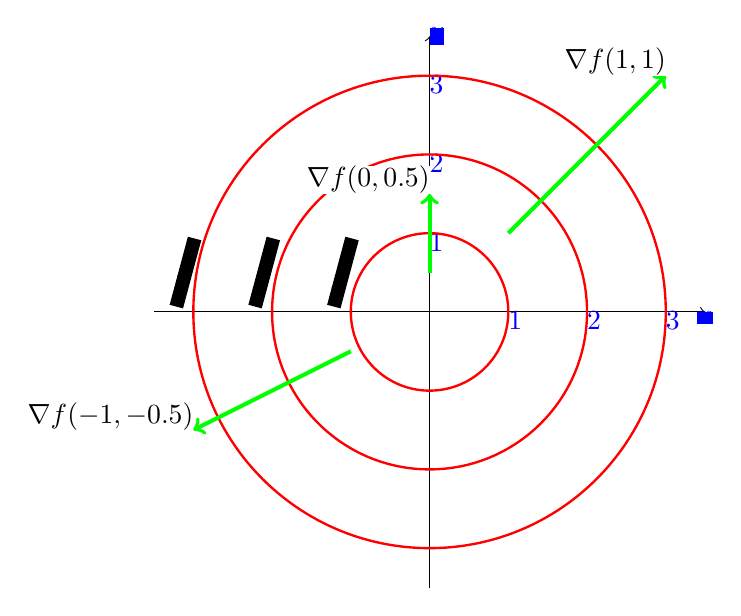
\begin{tikzpicture}

		\draw[->] (-3.5,0) -- (3.5,0) node[below] {$x$};
		\draw[->] (0,-3.5) -- (0,3.5) node[right] {$y$};

		\foreach \x in {1,2,3}
		\draw (\x,0) node[draw, inner sep=0pt, minimum size=0pt, minimum height = 4pt, label={below right:$\x$}] {};

		\foreach \x in {1,2,3}
		\draw (0,\x) node[draw, inner sep=0pt, minimum size=0pt, minimum width = 4pt, label={below right:$\x$}] {};

		\foreach \x in {1,2,3}
		\draw[red, line width=0.3mm] (0,0) circle (\x);
		\foreach \x/\y in {1/1,2/4,3/8}
		\draw (-\x-0.1,0.5) node[black, rotate=75] {\tiny$f(\x)=\y$};

		\foreach \x/\y in {1/1,0/0.5,-1/-0.5}
		\draw[green, ->, line width=0.5mm] (\x,\y) to (3*\x, 3*\y) node[above left, black, fill=white] {$\nabla f(\x,\y)$};
	\end{tikzpicture}
\end{center}

\subsection{Sätze zum totalen Differential}
\begin{satz}{}
	Existieren alle partiellen Ableitungen und sind diese stetig in $D$, dann ist die Ableitung $f:D\rightarrow\R^m$ total differenzierbar.
\end{satz}

\paragraph{Merkregel:}
\begin{center}
	
\begin{tikzpicture}
		\draw (0,0) node (spd) [draw] {stetig partiell differenzierbar};
	\end{tikzpicture}
\end{center}

\begin{satz}{Mittelwertsatz für reellwertige Funktionen}
	Sei $f:D\rightarrow\R,D\subseteq \R^n$ stetig differenzierbar in $D$ und $x,y$ sowie die Verbindungsstrecke $\overline{xy}=\set{x+t(y-x)}{t\in[0,1]}$ in $D$ enthalten. Dann exisitert ein $\xi\in\overline{xy}$, so dass
	\begin{equation*}
		f(y)-f(x)=Df(\xi)(y-x)
	\end{equation*}
	gilt. Dies verallgemeinert sich jedoch nicht auf vektorwertige Funktionen.
\end{satz}

\begin{satz}{Übertragung der Differenzierbarkeit}
	Sind $f$ und $g$ in $x$ total beziehungsweise partiell differenzierbar, dann sind auch $(f+g), (f-g)$ und $cf$ mit $c\in\R$ sowie falls $m=1$, $(f*g), \frac fg$ mit $g(x)\neq 0$ total beziehungsweise partiell differenzierbar.
\end{satz}

\begin{satz}{Mehrdimensionale Kettenregel}
	Seien $f:D\rightarrow\R^m,D\subseteq \R^n$ und $g:E\rightarrow\R^n,E\subseteq \R^k$ stetig differenzierbar mit $g(E)\subseteq D$, dann ist die Abbildung
	\begin{equation*}
		(f\circ g):E\rightarrow \R^m
	\end{equation*}
	stetig differenzierbar und es gilt die Kettenregel
	\begin{equation*}
		\frac{\diff}{\diff x}(f\circ g)(x)=f'(g(x))*g'(x)=D(f\circ g)(x)*Dg(x).
	\end{equation*}
\end{satz}
\paragraph{Beispiel:}
Seien $f:\R^2\rightarrow\R^2, f(x,y)=\vector{\sin(x)\\\cos(y)}, g:\R^3\rightarrow\R^2,g(x,y,z)=\vector{y^2\\x^3+z}$.
Damit ist
\begin{equation*}
	(f\circ g)(x,y,z)=\vector{\sin(y^2)\\\cos(x^3+z)}
\end{equation*}
und die einzelnen Jacobimatrizen der Funktionen sind
\begin{align*}
	\jacobi f(x,y)&=\matrix{\cos(x) & 0\\0 & -\sin(y)}
	& \jacobi g(x,y,z)&=\matrix{0 & 2y & 0\\3x^2 & 0 & 1}
\end{align*}
Weiter ist die Ableitung der Verkettung direkt ausgerechnet
\begin{equation*}
	D(f\circ g)(x,y,z)
	=\matrix{0&2y\cos(y^2)&0\\-3x^2\sin(x^3+z)&0&-\sin(x^3+z)}
\end{equation*}
Und nach der Kettenregel gilt
\begin{align*}
	D(f\circ g)&=Df(g(x,y,z))*Dg(x,y,z)\\
	&=\matrix{\cos(y^2) & 0\\0 & -\sin(x^3+z)}*\matrix{0 & 2y & 0\\3x^2 & 0 & 1}\\
	&=\matrix{0&2y\cos(y^2)&0\\-3x^2\sin(x^3+z)&0&-\sin(x^3+z)}\\
	&=D(f\circ g)(x,y,z)
\end{align*}

\section{Höhere Ableitungen im Mehrdimensionalen}
\begin{definition}{Höhere Ableitungen}
	Sei $f:D\rightarrow\R,D\subseteq\R^n$ partiell nach der Variablen $x_k$ differenzierbar, das heißt es existiert die Funktion
	\begin{equation*}
		\frac{\partial f}{\partial x_k}:D\rightarrow \R.
	\end{equation*}
	Besitzt diese wiederum eine partielle Ableitung nach der Variablen $x_i$, dann besitzt $f$ eine zweifache partielle Ableitung nach den Variablen $x_k$ und $x_i$. Wir schreiben
	\begin{equation*}
		\frac{\partial}{\partial x_i}\left(\frac{\partial f}{\partial x_k}\right)(x)=\frac{\partial^2 f}{\partial x_i\partial x_k}(x).
	\end{equation*}
	Falls $i=k$ ist, so schreiben wir $\frac{\partial^2 f}{\partial x_k^2}(x)$.
\end{definition}
Wichtige Frage ist, inwiefern spielt beim Bilden von höheren partiellen Ableitungen die Reihenfolge der Variablen eine Rolle?
\begin{satz}{Satz von Schwarz}
	Sei $f:D\rightarrow\R,D\subseteq\R^n$ eine stetige Funktion und die drei partiellen Ableitungen
	\begin{equation*}
		\frac{\partial f}{\partial x_i}(x),\ \frac{\partial f}{\partial x_k}(x) \text{ und } \frac{\partial^2 f}{\partial x_i\partial x_k}(x)
	\end{equation*}
	existieren und sind stetig, dann existiert auch die partielle Ableitung
	\begin{equation*}
		\frac{\partial^2 f}{\partial x_k\partial x_i}(x)
	\end{equation*}
	und es gilt
	\begin{equation*}
		\frac{\partial^2 f}{\partial x_i\partial x_k}(x)=\frac{\partial^2 f}{\partial x_k\partial x_i}(x).
	\end{equation*}
\end{satz}
Insbesondere gilt also, ist eine Funktion zweimal stetig partiell differenzierbar, dann kommt es beim Bilden von zweifachen partiellen Ableitungen nicht auf die Reihenfolge der Variablen an.
\paragraph{Folgerung:}
Insbesondere kommt es beim bilden von partiellen Ableitungen $k$ter Ordnung einer $k$fach stetig partiell differenzierbaren Funktion nicht auf die Reihenfolge an und man schreibt mit einem Multiindex
\begin{equation*}
	\alpha=(\alpha_1,\ldots,\alpha_n)\in \N_0^n
\end{equation*}
für die höheren Ableitungen
\begin{equation*}
	\frac{\partial^{|\alpha|}f}{\partial x^\alpha}(x)\coloneqq
	\frac{\partial^{|\alpha|}f}{\partial x_1^{\alpha_1}\partial x_2^{\alpha_2}\ldots\partial x_n^{\alpha_n}}(x)
\end{equation*}
einer $|\alpha|$fach stetig partiell differenzierbaren Funktion $f:D\rightarrow\R,D\subseteq\R^n$ wobei $|\alpha|=\alpha_1+\ldots+\alpha_n$ ist.

Zuletzt benötigen wir noch die zweite Ableitung im Mehrdimensionalen.

\begin{definition}{Hessematrix}
	Sei $f:D\rightarrow\R,D\subseteq\R^n$ zweimal stetig partiell differenzierbar. Dann definieren wir die \emph{Hesse'sche Matrix} von $f$ bei $x$ durch
	\begin{equation*}
		\newcommand{\partialF}[2]{\frac{\partial^2f}{\partial x_{#1}\partial x_{#2}}(x)}
		\renewcommand{\arraystretch}{1.7}
		\hess f(x)\coloneqq \begin{pmatrix}
			\partialF{1}{1} & \partialF{1}{2} & \cdots & \partialF{1}{n}\\
			\partialF{2}{1} & \partialF{2}{2} & \cdots & \partialF{2}{n}\\
			\vdots & \vdots & \ddots & \vdots\\
			\partialF{n}{1} & \partialF{n}{2} & \cdots & \partialF{n}{n}\\
		\end{pmatrix}=\left(\left( \partialF{i}{j}\right)\right)_{1\leq i,j\leq n}
	\end{equation*}
\end{definition}
Wir werden sehen, dass die Hessematrix ein Analogon der zweiten Ableitung $f''(x)$ im Eindimensionalen ist. Aus dem Satz von Schwarz folgt, dass die Hessematrix über die Hauptdiagonale symmetrisch ist.

\subsection{Taylorpolynom in mehreren Variablen}
\begin{satz}{Satz von Taylor}
	Sei $f:D\rightarrow\R,D\subseteq\R^n$ dreimal stetig partiell differenzierbar und $a\in D$. Dann gilt
	\begin{equation*}
		T(x)=f(a)+Df(a)(x-a)+\frac12 (x-a)^T\hess f(a)*(x-a)+o(|\!|x-a|\!|^2)
	\end{equation*}
	wobei $|\!|x-a|\!|$ den euklidischen Abstand von $x$ und $a$ bezeichnet. Man bezeichnet dies als das Taylorpolynom zweiter Ordnung.
\end{satz}
\paragraph{Beispiel:}
Sei $f:\R^2\rightarrow\R, f(x,y)=e^{x^2+y}$. Wir bestimmen das Taylorpolynom zweiter Ordnung im Punkt $a=(0,0)$. Wir bestimmen dafür
\begin{align*}
	f(a)=f(0,0)=1 && Df(x,y)&=\matrix{2xe^{x^2+y}&e^{x^2+y}}\\
	&&\Rightarrow\ Df(0,0)&=(0,1)
\end{align*}
und die Hessematrix von $f$
\begin{align*}
	\hess f(x,y)&=
	\matrix{
	2e^{x^2+y}+4x^2e^{x^2+y}
	&2xe^{x^2+y}
	\\2xe^{x^2+y}
	&e^{x^2+y}
	}\\
	\Rightarrow \hess f(0,0)=\matrix{2&0\\0&1}
\end{align*}
Damit ergibt sich für das Taylorpolynom schließlich
\begin{align*}
	T(x)&=f(a)+Df(a)(x-a)+\frac12 (x-a)^T\hess f(a)*(x-a)+o(|\!|x-a|\!|^2)\\
	&=1+(0,1)*\vector{x_1\\x_2}+\frac 12 (x_1,x_2)*\matrix{2&0\\0&1}*\vector{x_1\\x_2} + o(|\!|x|\!|^2)\\
	&=1+x_2+\frac 12 (2x_1,x_2)*\vector{x_1\\x_2} + o(|\!|x|\!|^2)\\
	&=1+x_2+\frac 12 (2x_1^2+x_2^2)\\
	&=1+x_2+x_1^2+\frac 12x_2^2\\
\end{align*}

